{
\makeatletter
\def\input@path{{../dyskretna}}
\makeatother
\graphicspath{{../dyskretna}}

% This has to be done, because we input another suffering with different sectioning scheme.
\let\realsection\section
\let\realsubsection\subsection
\let\section\subsection
\let\subsection\subsubsection
\let\subsubsection\paragraph

\chapter{Matematyka dyskretna} 
\section{Nieformalna definicja}
Tak jak w przypadku DFA i NFA mieliśmy automaty z jakimiś stanami, które przechodziły (albo nie) po kolejnych literach, tak automaty ze stosem mają jeszcze dodatkowo stos, na podstawie którego możemy podejmować decyzję co zrobić.

\section{Formalnie}
\begin{definition}
	\textbf{Automat ze stosem} (pushdown automaton PDA) definiujemy jako
	\[
		P = (Q, \Sigma, \Gamma, \delta, q_0, Z_0, F)
	\]
	gdzie
	\begin{itemize}
		\item \( Q \) -- zbiór stanów
		\item \( \Sigma \) -- skończony alfabet słów
		\item \( \Gamma \) -- skończony alfabet stosu
		\item \( \delta : Q \times (\Sigma \cup \set{\eps}) \times \Gamma \rightarrow \powerset\pars{Q \times \Gamma^*} \) -- funkcja przejścia
		\item \( q_0 \) -- stan startowy
		\item \( Z_0\) -- stosowy symbol startowy
		\item \( F \subseteq Q \) -- zbiór stanów akceptujących
	\end{itemize}
\end{definition}
Intuicyjnie \( \delta \) dla każdego stanu \( q \), litery \( a \), symbolu na szczycie stosu \( z \) oddaje zbiór nowych stanów wraz z symbolami które mają być dodane na stos.
Symbol \( z \) jest usuwany ze szczytu stosu w momencie przejścia, wiele nowych symboli może zostać dodanych.
Jeśli zdarzy się, że opróżnimy stos to mamy tak zwany przypał, ale się tym nie przejmujemy.

\begin{definition}
	\textbf{Konfiguracja} PDA to trójka
	\[
		(q, w, \gamma)
	\]
	gdzie
	\begin{itemize}
		\item \( q \) -- aktualny stan
		\item \( w \) -- część słowa pozostała do przeczytania
		\item \( \gamma \) -- (wszystkie) symbole na stosie
	\end{itemize}
\end{definition}

\begin{definition}
	Dla konfiguracji PDA \( P \) definiujemy relację \( \vdash_P \)
	\[
		(q, aw, X\beta) \vdash_P (p, w, \alpha \beta)
		\iff
		(p, \alpha) \in \delta(q, a, X)
	\]
\end{definition}

\begin{definition}
	Definiujemy \( \vdash_P^* \) jako zwrotne i przechodnie domknięcie \( \vdash_P \)
\end{definition}

\begin{lemma}
	Dla PDA \( P \) jeśli
	\[
		(q, x, \alpha) \vdash_P^* (p, y, \beta)
	\]
	to
	\[
		(q, xw, \alpha\gamma) \vdash_P^* (p, yw, \beta\gamma)
	\]
\end{lemma}

\section{Akceptacja}
\subsection{Akceptacja stanem akceptującym}
\[
	L(P) = \set{ w \mid (q_0, w, Z_0) \vdash_P^* (q_F, \eps, \gamma) \land q_F \in F}
\]

\subsection{Akceptacja pustym stosem}
\[
	N(P) = \set{ w \mid (q_0, w, Z_0) \vdash_P^* (q, \eps, \eps)}
\]

\subsection{Równoważność}
Mamy dwie różne definicje tego co znaczy, że jakieś słowo jest akceptowane -- pytanie czy są one równoważne tj. czy jeśli mamy słowo \( w \in L(P) \) to umiemy skonstruować automat \( Q \) taki że \( w \in N(Q)  \) i na odwrót.

Z \( P, L(P) \) łatwo jesteśmy w stanie skonstruować \( Q, N(Q) \) -- jeśli stan \( q_F \) był akceptujący to przechodzimy do stanu, który epsilon przejściami opróżniamy stos.

Z \( Q, N(Q) \)





\realsection{Zasada włączeń i wyłączeń. Przykłady zastosowań}
 % Żeby nie było syfu to kolejne sekcje dodajemy do chapters/
% A potem includujemy za pomocą \input{chapters/...}

% Używamy \( \) i \[ \] zamiast dolarów -- tak jak się robi w LaTeXu


\documentclass[12pt, a4paper, polish, openany]{book}

% Please, let's familiarize ourselves with notatki.sty and tcs.sty so that we don't reinvent the wheel
\usepackage{notatki}
\fancyhead[L]{\textbf{\textit{MPI}}}

\begin{document}
% Front page and table of contents
\frontmatter

\begin{titlepage}

	\begin{center}
		\begin{figure}[h]
			\centering
			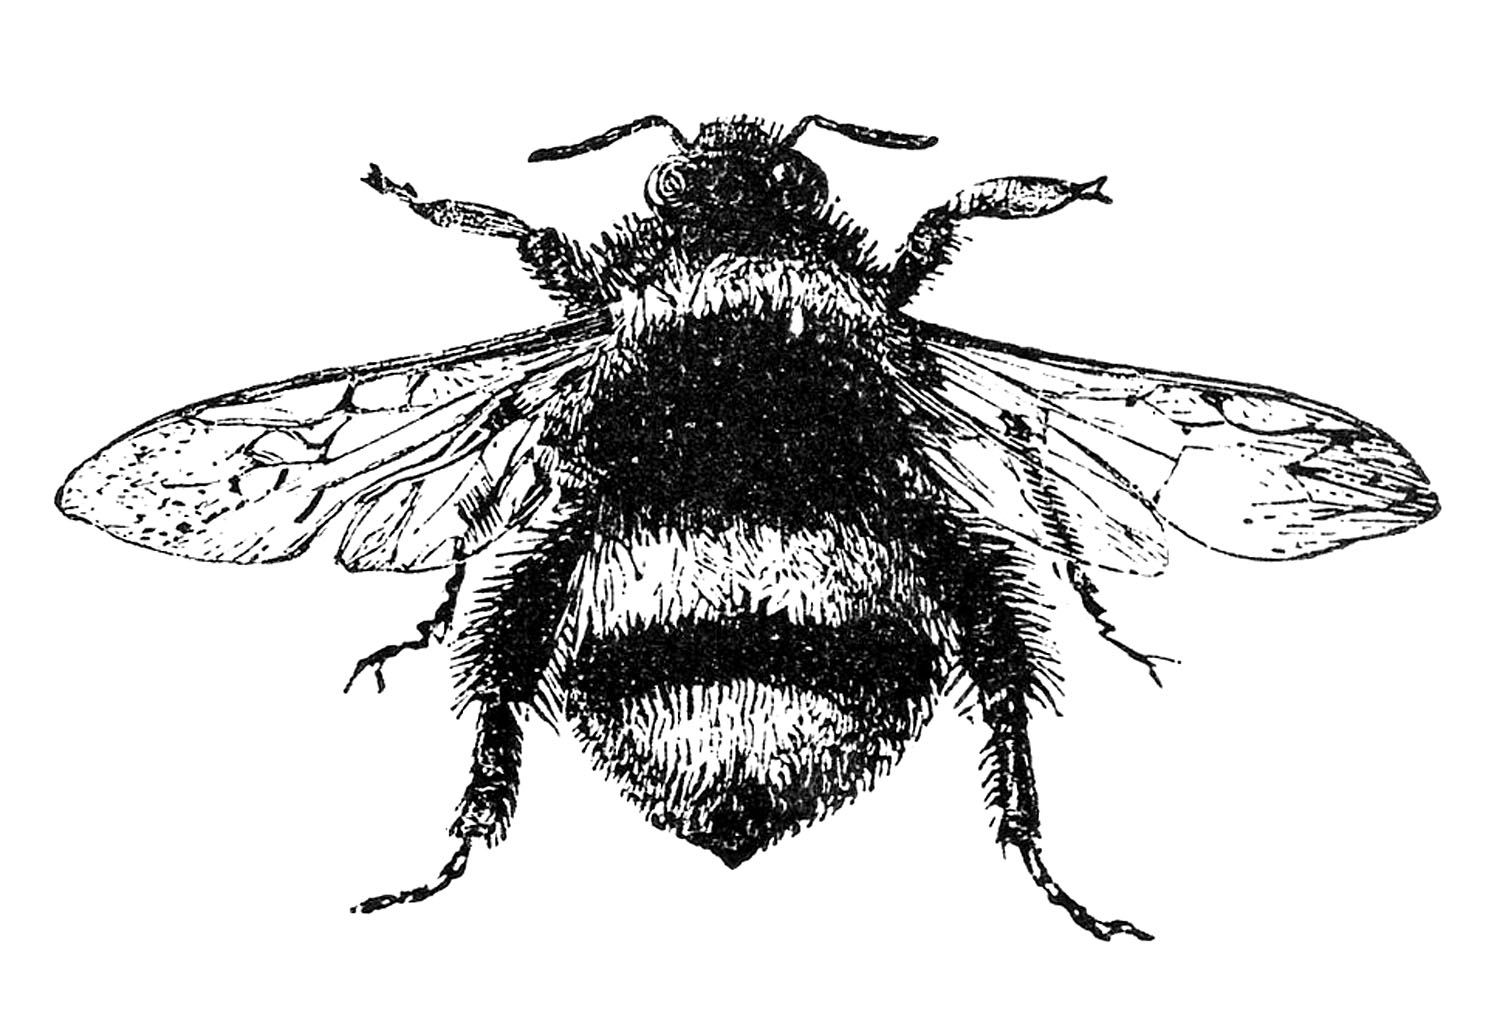
\includegraphics[scale=0.75]{img/bumblebee.jpg}
		\end{figure}
		\vspace{0.5cm}
		\Huge
		\textbf{\textsc{Metody Probabilistyczne Informatyki}}

		\vspace{0.5cm}
		\Large
		\textsc{Wybrane Dowody}

		\normalsize


		\line(1,0){330}

		\vspace{1cm}
		\textit{,,Tak teraz na to patrzę i myślę, czy ta nierówność nie powinna być w drugą stronę...''}
		\vspace{1cm}

		\textit{\textsc{Popełnione przez}}\\
		\vspace{5mm}

		\textbf{\textsc{
				Załatany Ponton \\
				V\\
				Nahtamatu\\
			}}

		\vfill

		Kraków \\
		Anno Domini 2025

	\end{center}

\end{titlepage}


\tableofcontents
\section*{Licencja}
\begin{figure}[h]
	\begin{minipage}[c]{0.25\textwidth}
		
\includegraphics[width=0.7\textwidth]{img/licencja.png}
	\end{minipage}\hfill
	\begin{minipage}[c]{0.75\textwidth}
		\caption*{
			Ten utwór jest dostępny na
			\href{https://creativecommons.org/licenses/by-sa/4.0/}{licencji Creative Commons Uznanie autorstwa
				na tych samych warunkach 4.0 Międzynarodowe.}
		}
	\end{minipage}
\end{figure}

% Remove the "Rozdział x" chapter headings, as we already number our chapters
\titleformat{\chapter}[display]{\normalfont\Huge\bfseries}{}{0pt}{\Huge}
\titlespacing*{\chapter}{0pt}{0pt}{20pt}

% Actual content
\mainmatter

\chapter{Wykład 1 (2025-10-03)}
 % Żeby nie było syfu to kolejne sekcje dodajemy do chapters/
% A potem includujemy za pomocą \input{chapters/...}

% Używamy \( \) i \[ \] zamiast dolarów -- tak jak się robi w LaTeXu


\documentclass[12pt, a4paper, polish, openany]{book}

% Please, let's familiarize ourselves with notatki.sty and tcs.sty so that we don't reinvent the wheel
\usepackage{notatki}
\fancyhead[L]{\textbf{\textit{MPI}}}

\begin{document}
% Front page and table of contents
\frontmatter

\begin{titlepage}

	\begin{center}
		\begin{figure}[h]
			\centering
			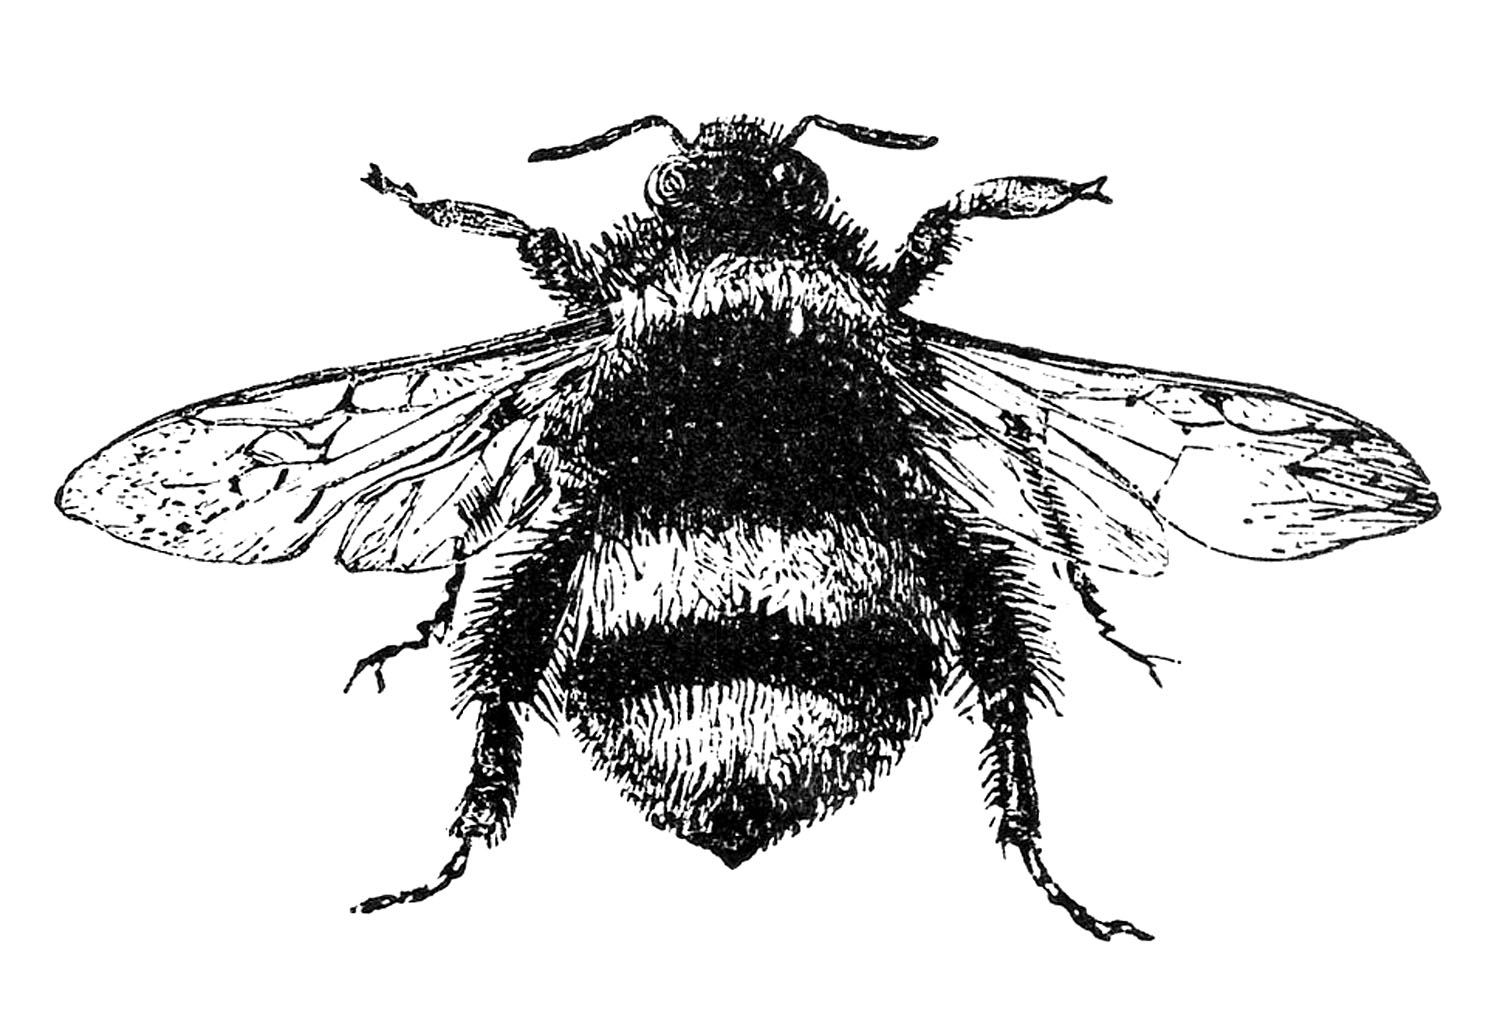
\includegraphics[scale=0.75]{img/bumblebee.jpg}
		\end{figure}
		\vspace{0.5cm}
		\Huge
		\textbf{\textsc{Metody Probabilistyczne Informatyki}}

		\vspace{0.5cm}
		\Large
		\textsc{Wybrane Dowody}

		\normalsize


		\line(1,0){330}

		\vspace{1cm}
		\textit{,,Tak teraz na to patrzę i myślę, czy ta nierówność nie powinna być w drugą stronę...''}
		\vspace{1cm}

		\textit{\textsc{Popełnione przez}}\\
		\vspace{5mm}

		\textbf{\textsc{
				Załatany Ponton \\
				V\\
				Nahtamatu\\
			}}

		\vfill

		Kraków \\
		Anno Domini 2025

	\end{center}

\end{titlepage}


\tableofcontents
\section*{Licencja}
\begin{figure}[h]
	\begin{minipage}[c]{0.25\textwidth}
		
\includegraphics[width=0.7\textwidth]{img/licencja.png}
	\end{minipage}\hfill
	\begin{minipage}[c]{0.75\textwidth}
		\caption*{
			Ten utwór jest dostępny na
			\href{https://creativecommons.org/licenses/by-sa/4.0/}{licencji Creative Commons Uznanie autorstwa
				na tych samych warunkach 4.0 Międzynarodowe.}
		}
	\end{minipage}
\end{figure}

% Remove the "Rozdział x" chapter headings, as we already number our chapters
\titleformat{\chapter}[display]{\normalfont\Huge\bfseries}{}{0pt}{\Huge}
\titlespacing*{\chapter}{0pt}{0pt}{20pt}

% Actual content
\mainmatter

\chapter{Wykład 1 (2025-10-03)}
 % Żeby nie było syfu to kolejne sekcje dodajemy do chapters/
% A potem includujemy za pomocą \input{chapters/...}

% Używamy \( \) i \[ \] zamiast dolarów -- tak jak się robi w LaTeXu


\documentclass[12pt, a4paper, polish, openany]{book}

% Please, let's familiarize ourselves with notatki.sty and tcs.sty so that we don't reinvent the wheel
\usepackage{notatki}
\fancyhead[L]{\textbf{\textit{MPI}}}

\begin{document}
% Front page and table of contents
\frontmatter

\input{titlepage}

\tableofcontents
\input{license}

% Remove the "Rozdział x" chapter headings, as we already number our chapters
\titleformat{\chapter}[display]{\normalfont\Huge\bfseries}{}{0pt}{\Huge}
\titlespacing*{\chapter}{0pt}{0pt}{20pt}

% Actual content
\mainmatter

\chapter{Wykład 1 (2025-10-03)}
\input{chapters/2025-10-03-lecture/main}

\chapter{Nagranie 1 (2025-10-04)}
\input{chapters/2025-10-04-recording/main}

\chapter{Wykład 2 (2025-10-10)}
\input{chapters/2025-10-10-lecture/main}

\chapter{Nagranie 2 (2025-10-10)}
\input{chapters/2025-10-10-recording/main}

\chapter{Wykład 3 (2025-10-17)}
\input{chapters/2025-10-17-lecture/main}

\end{document}


\chapter{Nagranie 1 (2025-10-04)}
 % Żeby nie było syfu to kolejne sekcje dodajemy do chapters/
% A potem includujemy za pomocą \input{chapters/...}

% Używamy \( \) i \[ \] zamiast dolarów -- tak jak się robi w LaTeXu


\documentclass[12pt, a4paper, polish, openany]{book}

% Please, let's familiarize ourselves with notatki.sty and tcs.sty so that we don't reinvent the wheel
\usepackage{notatki}
\fancyhead[L]{\textbf{\textit{MPI}}}

\begin{document}
% Front page and table of contents
\frontmatter

\input{titlepage}

\tableofcontents
\input{license}

% Remove the "Rozdział x" chapter headings, as we already number our chapters
\titleformat{\chapter}[display]{\normalfont\Huge\bfseries}{}{0pt}{\Huge}
\titlespacing*{\chapter}{0pt}{0pt}{20pt}

% Actual content
\mainmatter

\chapter{Wykład 1 (2025-10-03)}
\input{chapters/2025-10-03-lecture/main}

\chapter{Nagranie 1 (2025-10-04)}
\input{chapters/2025-10-04-recording/main}

\chapter{Wykład 2 (2025-10-10)}
\input{chapters/2025-10-10-lecture/main}

\chapter{Nagranie 2 (2025-10-10)}
\input{chapters/2025-10-10-recording/main}

\chapter{Wykład 3 (2025-10-17)}
\input{chapters/2025-10-17-lecture/main}

\end{document}


\chapter{Wykład 2 (2025-10-10)}
 % Żeby nie było syfu to kolejne sekcje dodajemy do chapters/
% A potem includujemy za pomocą \input{chapters/...}

% Używamy \( \) i \[ \] zamiast dolarów -- tak jak się robi w LaTeXu


\documentclass[12pt, a4paper, polish, openany]{book}

% Please, let's familiarize ourselves with notatki.sty and tcs.sty so that we don't reinvent the wheel
\usepackage{notatki}
\fancyhead[L]{\textbf{\textit{MPI}}}

\begin{document}
% Front page and table of contents
\frontmatter

\input{titlepage}

\tableofcontents
\input{license}

% Remove the "Rozdział x" chapter headings, as we already number our chapters
\titleformat{\chapter}[display]{\normalfont\Huge\bfseries}{}{0pt}{\Huge}
\titlespacing*{\chapter}{0pt}{0pt}{20pt}

% Actual content
\mainmatter

\chapter{Wykład 1 (2025-10-03)}
\input{chapters/2025-10-03-lecture/main}

\chapter{Nagranie 1 (2025-10-04)}
\input{chapters/2025-10-04-recording/main}

\chapter{Wykład 2 (2025-10-10)}
\input{chapters/2025-10-10-lecture/main}

\chapter{Nagranie 2 (2025-10-10)}
\input{chapters/2025-10-10-recording/main}

\chapter{Wykład 3 (2025-10-17)}
\input{chapters/2025-10-17-lecture/main}

\end{document}


\chapter{Nagranie 2 (2025-10-10)}
 % Żeby nie było syfu to kolejne sekcje dodajemy do chapters/
% A potem includujemy za pomocą \input{chapters/...}

% Używamy \( \) i \[ \] zamiast dolarów -- tak jak się robi w LaTeXu


\documentclass[12pt, a4paper, polish, openany]{book}

% Please, let's familiarize ourselves with notatki.sty and tcs.sty so that we don't reinvent the wheel
\usepackage{notatki}
\fancyhead[L]{\textbf{\textit{MPI}}}

\begin{document}
% Front page and table of contents
\frontmatter

\input{titlepage}

\tableofcontents
\input{license}

% Remove the "Rozdział x" chapter headings, as we already number our chapters
\titleformat{\chapter}[display]{\normalfont\Huge\bfseries}{}{0pt}{\Huge}
\titlespacing*{\chapter}{0pt}{0pt}{20pt}

% Actual content
\mainmatter

\chapter{Wykład 1 (2025-10-03)}
\input{chapters/2025-10-03-lecture/main}

\chapter{Nagranie 1 (2025-10-04)}
\input{chapters/2025-10-04-recording/main}

\chapter{Wykład 2 (2025-10-10)}
\input{chapters/2025-10-10-lecture/main}

\chapter{Nagranie 2 (2025-10-10)}
\input{chapters/2025-10-10-recording/main}

\chapter{Wykład 3 (2025-10-17)}
\input{chapters/2025-10-17-lecture/main}

\end{document}


\chapter{Wykład 3 (2025-10-17)}
 % Żeby nie było syfu to kolejne sekcje dodajemy do chapters/
% A potem includujemy za pomocą \input{chapters/...}

% Używamy \( \) i \[ \] zamiast dolarów -- tak jak się robi w LaTeXu


\documentclass[12pt, a4paper, polish, openany]{book}

% Please, let's familiarize ourselves with notatki.sty and tcs.sty so that we don't reinvent the wheel
\usepackage{notatki}
\fancyhead[L]{\textbf{\textit{MPI}}}

\begin{document}
% Front page and table of contents
\frontmatter

\input{titlepage}

\tableofcontents
\input{license}

% Remove the "Rozdział x" chapter headings, as we already number our chapters
\titleformat{\chapter}[display]{\normalfont\Huge\bfseries}{}{0pt}{\Huge}
\titlespacing*{\chapter}{0pt}{0pt}{20pt}

% Actual content
\mainmatter

\chapter{Wykład 1 (2025-10-03)}
\input{chapters/2025-10-03-lecture/main}

\chapter{Nagranie 1 (2025-10-04)}
\input{chapters/2025-10-04-recording/main}

\chapter{Wykład 2 (2025-10-10)}
\input{chapters/2025-10-10-lecture/main}

\chapter{Nagranie 2 (2025-10-10)}
\input{chapters/2025-10-10-recording/main}

\chapter{Wykład 3 (2025-10-17)}
\input{chapters/2025-10-17-lecture/main}

\end{document}


\end{document}


\chapter{Nagranie 1 (2025-10-04)}
 % Żeby nie było syfu to kolejne sekcje dodajemy do chapters/
% A potem includujemy za pomocą \input{chapters/...}

% Używamy \( \) i \[ \] zamiast dolarów -- tak jak się robi w LaTeXu


\documentclass[12pt, a4paper, polish, openany]{book}

% Please, let's familiarize ourselves with notatki.sty and tcs.sty so that we don't reinvent the wheel
\usepackage{notatki}
\fancyhead[L]{\textbf{\textit{MPI}}}

\begin{document}
% Front page and table of contents
\frontmatter

\begin{titlepage}

	\begin{center}
		\begin{figure}[h]
			\centering
			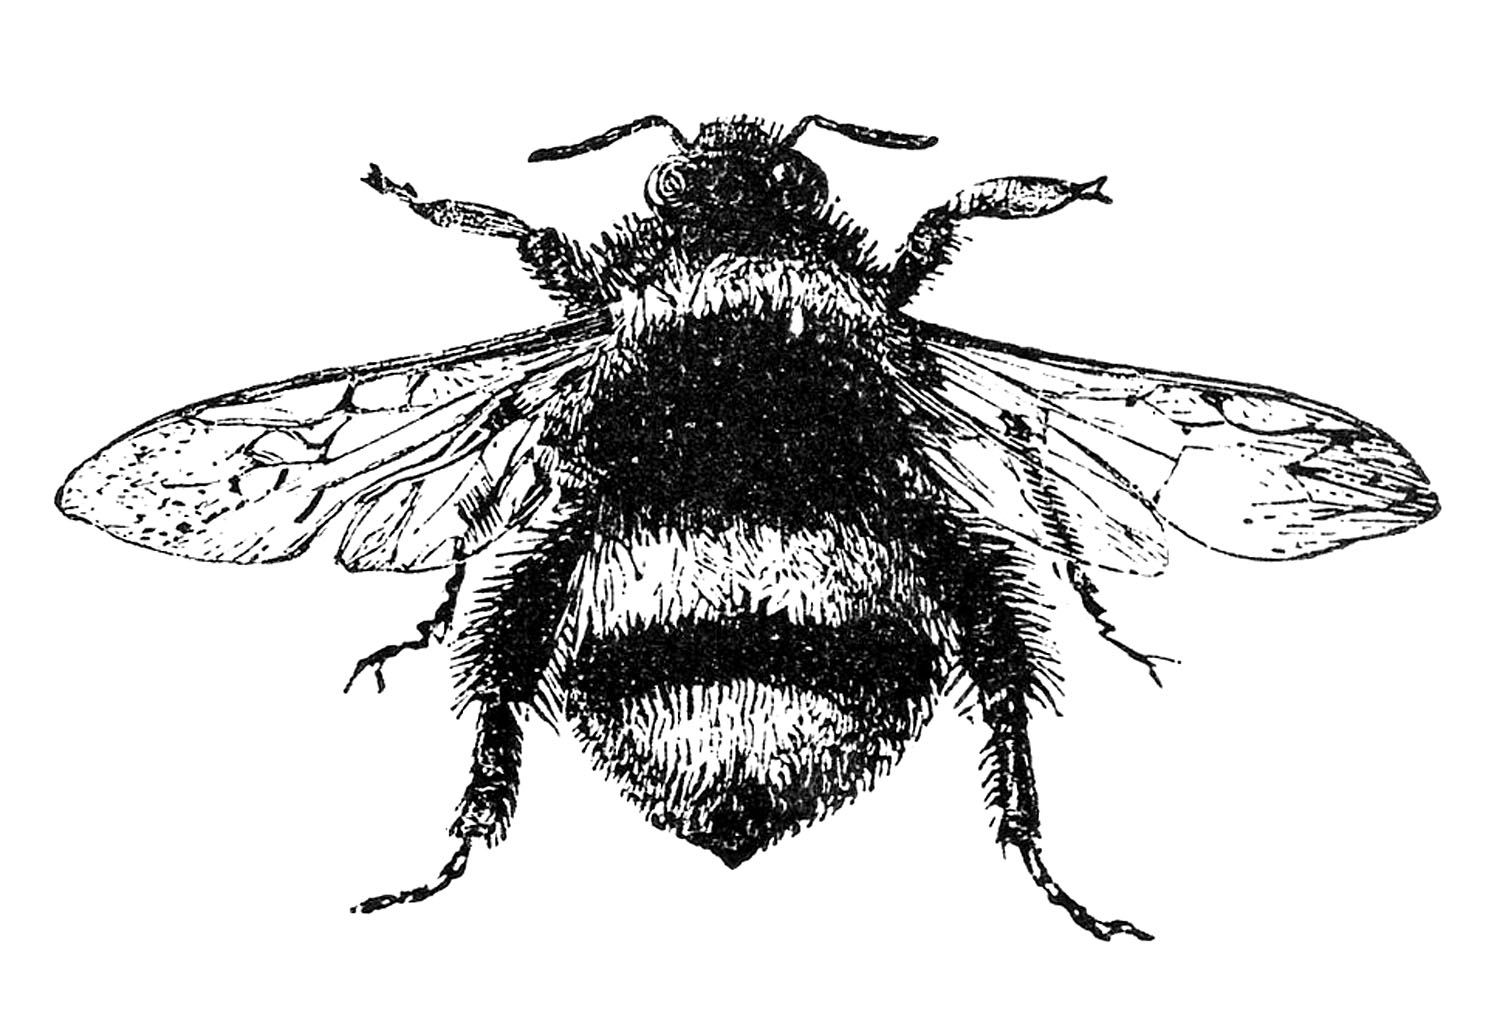
\includegraphics[scale=0.75]{img/bumblebee.jpg}
		\end{figure}
		\vspace{0.5cm}
		\Huge
		\textbf{\textsc{Metody Probabilistyczne Informatyki}}

		\vspace{0.5cm}
		\Large
		\textsc{Wybrane Dowody}

		\normalsize


		\line(1,0){330}

		\vspace{1cm}
		\textit{,,Tak teraz na to patrzę i myślę, czy ta nierówność nie powinna być w drugą stronę...''}
		\vspace{1cm}

		\textit{\textsc{Popełnione przez}}\\
		\vspace{5mm}

		\textbf{\textsc{
				Załatany Ponton \\
				V\\
				Nahtamatu\\
			}}

		\vfill

		Kraków \\
		Anno Domini 2025

	\end{center}

\end{titlepage}


\tableofcontents
\section*{Licencja}
\begin{figure}[h]
	\begin{minipage}[c]{0.25\textwidth}
		
\includegraphics[width=0.7\textwidth]{img/licencja.png}
	\end{minipage}\hfill
	\begin{minipage}[c]{0.75\textwidth}
		\caption*{
			Ten utwór jest dostępny na
			\href{https://creativecommons.org/licenses/by-sa/4.0/}{licencji Creative Commons Uznanie autorstwa
				na tych samych warunkach 4.0 Międzynarodowe.}
		}
	\end{minipage}
\end{figure}

% Remove the "Rozdział x" chapter headings, as we already number our chapters
\titleformat{\chapter}[display]{\normalfont\Huge\bfseries}{}{0pt}{\Huge}
\titlespacing*{\chapter}{0pt}{0pt}{20pt}

% Actual content
\mainmatter

\chapter{Wykład 1 (2025-10-03)}
 % Żeby nie było syfu to kolejne sekcje dodajemy do chapters/
% A potem includujemy za pomocą \input{chapters/...}

% Używamy \( \) i \[ \] zamiast dolarów -- tak jak się robi w LaTeXu


\documentclass[12pt, a4paper, polish, openany]{book}

% Please, let's familiarize ourselves with notatki.sty and tcs.sty so that we don't reinvent the wheel
\usepackage{notatki}
\fancyhead[L]{\textbf{\textit{MPI}}}

\begin{document}
% Front page and table of contents
\frontmatter

\input{titlepage}

\tableofcontents
\input{license}

% Remove the "Rozdział x" chapter headings, as we already number our chapters
\titleformat{\chapter}[display]{\normalfont\Huge\bfseries}{}{0pt}{\Huge}
\titlespacing*{\chapter}{0pt}{0pt}{20pt}

% Actual content
\mainmatter

\chapter{Wykład 1 (2025-10-03)}
\input{chapters/2025-10-03-lecture/main}

\chapter{Nagranie 1 (2025-10-04)}
\input{chapters/2025-10-04-recording/main}

\chapter{Wykład 2 (2025-10-10)}
\input{chapters/2025-10-10-lecture/main}

\chapter{Nagranie 2 (2025-10-10)}
\input{chapters/2025-10-10-recording/main}

\chapter{Wykład 3 (2025-10-17)}
\input{chapters/2025-10-17-lecture/main}

\end{document}


\chapter{Nagranie 1 (2025-10-04)}
 % Żeby nie było syfu to kolejne sekcje dodajemy do chapters/
% A potem includujemy za pomocą \input{chapters/...}

% Używamy \( \) i \[ \] zamiast dolarów -- tak jak się robi w LaTeXu


\documentclass[12pt, a4paper, polish, openany]{book}

% Please, let's familiarize ourselves with notatki.sty and tcs.sty so that we don't reinvent the wheel
\usepackage{notatki}
\fancyhead[L]{\textbf{\textit{MPI}}}

\begin{document}
% Front page and table of contents
\frontmatter

\input{titlepage}

\tableofcontents
\input{license}

% Remove the "Rozdział x" chapter headings, as we already number our chapters
\titleformat{\chapter}[display]{\normalfont\Huge\bfseries}{}{0pt}{\Huge}
\titlespacing*{\chapter}{0pt}{0pt}{20pt}

% Actual content
\mainmatter

\chapter{Wykład 1 (2025-10-03)}
\input{chapters/2025-10-03-lecture/main}

\chapter{Nagranie 1 (2025-10-04)}
\input{chapters/2025-10-04-recording/main}

\chapter{Wykład 2 (2025-10-10)}
\input{chapters/2025-10-10-lecture/main}

\chapter{Nagranie 2 (2025-10-10)}
\input{chapters/2025-10-10-recording/main}

\chapter{Wykład 3 (2025-10-17)}
\input{chapters/2025-10-17-lecture/main}

\end{document}


\chapter{Wykład 2 (2025-10-10)}
 % Żeby nie było syfu to kolejne sekcje dodajemy do chapters/
% A potem includujemy za pomocą \input{chapters/...}

% Używamy \( \) i \[ \] zamiast dolarów -- tak jak się robi w LaTeXu


\documentclass[12pt, a4paper, polish, openany]{book}

% Please, let's familiarize ourselves with notatki.sty and tcs.sty so that we don't reinvent the wheel
\usepackage{notatki}
\fancyhead[L]{\textbf{\textit{MPI}}}

\begin{document}
% Front page and table of contents
\frontmatter

\input{titlepage}

\tableofcontents
\input{license}

% Remove the "Rozdział x" chapter headings, as we already number our chapters
\titleformat{\chapter}[display]{\normalfont\Huge\bfseries}{}{0pt}{\Huge}
\titlespacing*{\chapter}{0pt}{0pt}{20pt}

% Actual content
\mainmatter

\chapter{Wykład 1 (2025-10-03)}
\input{chapters/2025-10-03-lecture/main}

\chapter{Nagranie 1 (2025-10-04)}
\input{chapters/2025-10-04-recording/main}

\chapter{Wykład 2 (2025-10-10)}
\input{chapters/2025-10-10-lecture/main}

\chapter{Nagranie 2 (2025-10-10)}
\input{chapters/2025-10-10-recording/main}

\chapter{Wykład 3 (2025-10-17)}
\input{chapters/2025-10-17-lecture/main}

\end{document}


\chapter{Nagranie 2 (2025-10-10)}
 % Żeby nie było syfu to kolejne sekcje dodajemy do chapters/
% A potem includujemy za pomocą \input{chapters/...}

% Używamy \( \) i \[ \] zamiast dolarów -- tak jak się robi w LaTeXu


\documentclass[12pt, a4paper, polish, openany]{book}

% Please, let's familiarize ourselves with notatki.sty and tcs.sty so that we don't reinvent the wheel
\usepackage{notatki}
\fancyhead[L]{\textbf{\textit{MPI}}}

\begin{document}
% Front page and table of contents
\frontmatter

\input{titlepage}

\tableofcontents
\input{license}

% Remove the "Rozdział x" chapter headings, as we already number our chapters
\titleformat{\chapter}[display]{\normalfont\Huge\bfseries}{}{0pt}{\Huge}
\titlespacing*{\chapter}{0pt}{0pt}{20pt}

% Actual content
\mainmatter

\chapter{Wykład 1 (2025-10-03)}
\input{chapters/2025-10-03-lecture/main}

\chapter{Nagranie 1 (2025-10-04)}
\input{chapters/2025-10-04-recording/main}

\chapter{Wykład 2 (2025-10-10)}
\input{chapters/2025-10-10-lecture/main}

\chapter{Nagranie 2 (2025-10-10)}
\input{chapters/2025-10-10-recording/main}

\chapter{Wykład 3 (2025-10-17)}
\input{chapters/2025-10-17-lecture/main}

\end{document}


\chapter{Wykład 3 (2025-10-17)}
 % Żeby nie było syfu to kolejne sekcje dodajemy do chapters/
% A potem includujemy za pomocą \input{chapters/...}

% Używamy \( \) i \[ \] zamiast dolarów -- tak jak się robi w LaTeXu


\documentclass[12pt, a4paper, polish, openany]{book}

% Please, let's familiarize ourselves with notatki.sty and tcs.sty so that we don't reinvent the wheel
\usepackage{notatki}
\fancyhead[L]{\textbf{\textit{MPI}}}

\begin{document}
% Front page and table of contents
\frontmatter

\input{titlepage}

\tableofcontents
\input{license}

% Remove the "Rozdział x" chapter headings, as we already number our chapters
\titleformat{\chapter}[display]{\normalfont\Huge\bfseries}{}{0pt}{\Huge}
\titlespacing*{\chapter}{0pt}{0pt}{20pt}

% Actual content
\mainmatter

\chapter{Wykład 1 (2025-10-03)}
\input{chapters/2025-10-03-lecture/main}

\chapter{Nagranie 1 (2025-10-04)}
\input{chapters/2025-10-04-recording/main}

\chapter{Wykład 2 (2025-10-10)}
\input{chapters/2025-10-10-lecture/main}

\chapter{Nagranie 2 (2025-10-10)}
\input{chapters/2025-10-10-recording/main}

\chapter{Wykład 3 (2025-10-17)}
\input{chapters/2025-10-17-lecture/main}

\end{document}


\end{document}


\chapter{Wykład 2 (2025-10-10)}
 % Żeby nie było syfu to kolejne sekcje dodajemy do chapters/
% A potem includujemy za pomocą \input{chapters/...}

% Używamy \( \) i \[ \] zamiast dolarów -- tak jak się robi w LaTeXu


\documentclass[12pt, a4paper, polish, openany]{book}

% Please, let's familiarize ourselves with notatki.sty and tcs.sty so that we don't reinvent the wheel
\usepackage{notatki}
\fancyhead[L]{\textbf{\textit{MPI}}}

\begin{document}
% Front page and table of contents
\frontmatter

\begin{titlepage}

	\begin{center}
		\begin{figure}[h]
			\centering
			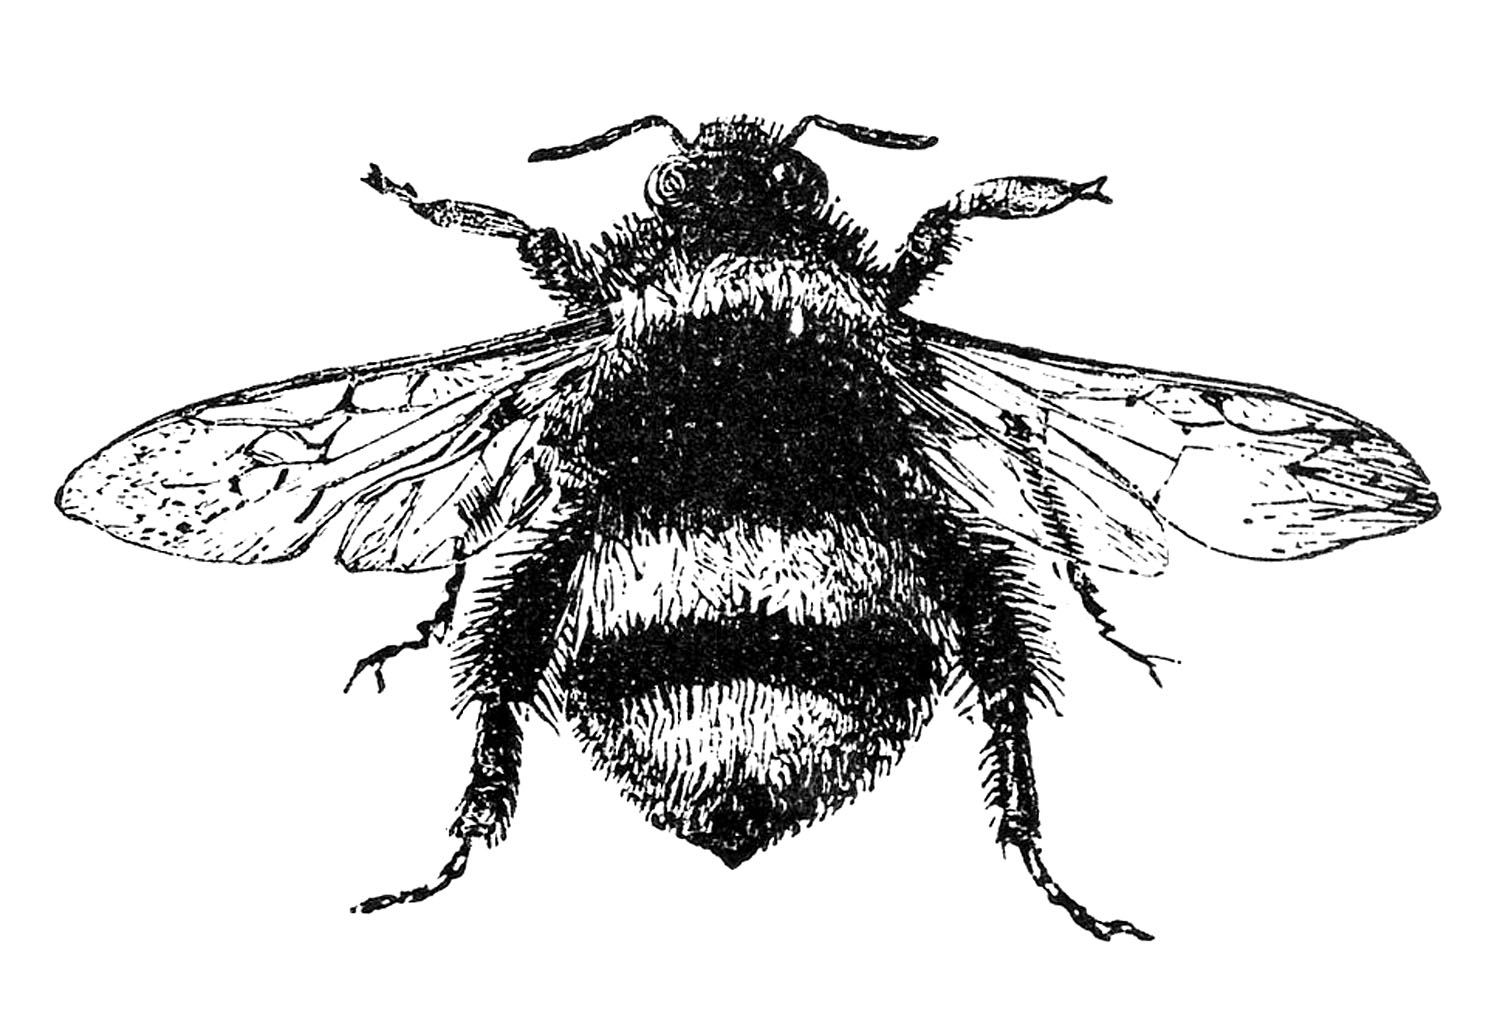
\includegraphics[scale=0.75]{img/bumblebee.jpg}
		\end{figure}
		\vspace{0.5cm}
		\Huge
		\textbf{\textsc{Metody Probabilistyczne Informatyki}}

		\vspace{0.5cm}
		\Large
		\textsc{Wybrane Dowody}

		\normalsize


		\line(1,0){330}

		\vspace{1cm}
		\textit{,,Tak teraz na to patrzę i myślę, czy ta nierówność nie powinna być w drugą stronę...''}
		\vspace{1cm}

		\textit{\textsc{Popełnione przez}}\\
		\vspace{5mm}

		\textbf{\textsc{
				Załatany Ponton \\
				V\\
				Nahtamatu\\
			}}

		\vfill

		Kraków \\
		Anno Domini 2025

	\end{center}

\end{titlepage}


\tableofcontents
\section*{Licencja}
\begin{figure}[h]
	\begin{minipage}[c]{0.25\textwidth}
		
\includegraphics[width=0.7\textwidth]{img/licencja.png}
	\end{minipage}\hfill
	\begin{minipage}[c]{0.75\textwidth}
		\caption*{
			Ten utwór jest dostępny na
			\href{https://creativecommons.org/licenses/by-sa/4.0/}{licencji Creative Commons Uznanie autorstwa
				na tych samych warunkach 4.0 Międzynarodowe.}
		}
	\end{minipage}
\end{figure}

% Remove the "Rozdział x" chapter headings, as we already number our chapters
\titleformat{\chapter}[display]{\normalfont\Huge\bfseries}{}{0pt}{\Huge}
\titlespacing*{\chapter}{0pt}{0pt}{20pt}

% Actual content
\mainmatter

\chapter{Wykład 1 (2025-10-03)}
 % Żeby nie było syfu to kolejne sekcje dodajemy do chapters/
% A potem includujemy za pomocą \input{chapters/...}

% Używamy \( \) i \[ \] zamiast dolarów -- tak jak się robi w LaTeXu


\documentclass[12pt, a4paper, polish, openany]{book}

% Please, let's familiarize ourselves with notatki.sty and tcs.sty so that we don't reinvent the wheel
\usepackage{notatki}
\fancyhead[L]{\textbf{\textit{MPI}}}

\begin{document}
% Front page and table of contents
\frontmatter

\input{titlepage}

\tableofcontents
\input{license}

% Remove the "Rozdział x" chapter headings, as we already number our chapters
\titleformat{\chapter}[display]{\normalfont\Huge\bfseries}{}{0pt}{\Huge}
\titlespacing*{\chapter}{0pt}{0pt}{20pt}

% Actual content
\mainmatter

\chapter{Wykład 1 (2025-10-03)}
\input{chapters/2025-10-03-lecture/main}

\chapter{Nagranie 1 (2025-10-04)}
\input{chapters/2025-10-04-recording/main}

\chapter{Wykład 2 (2025-10-10)}
\input{chapters/2025-10-10-lecture/main}

\chapter{Nagranie 2 (2025-10-10)}
\input{chapters/2025-10-10-recording/main}

\chapter{Wykład 3 (2025-10-17)}
\input{chapters/2025-10-17-lecture/main}

\end{document}


\chapter{Nagranie 1 (2025-10-04)}
 % Żeby nie było syfu to kolejne sekcje dodajemy do chapters/
% A potem includujemy za pomocą \input{chapters/...}

% Używamy \( \) i \[ \] zamiast dolarów -- tak jak się robi w LaTeXu


\documentclass[12pt, a4paper, polish, openany]{book}

% Please, let's familiarize ourselves with notatki.sty and tcs.sty so that we don't reinvent the wheel
\usepackage{notatki}
\fancyhead[L]{\textbf{\textit{MPI}}}

\begin{document}
% Front page and table of contents
\frontmatter

\input{titlepage}

\tableofcontents
\input{license}

% Remove the "Rozdział x" chapter headings, as we already number our chapters
\titleformat{\chapter}[display]{\normalfont\Huge\bfseries}{}{0pt}{\Huge}
\titlespacing*{\chapter}{0pt}{0pt}{20pt}

% Actual content
\mainmatter

\chapter{Wykład 1 (2025-10-03)}
\input{chapters/2025-10-03-lecture/main}

\chapter{Nagranie 1 (2025-10-04)}
\input{chapters/2025-10-04-recording/main}

\chapter{Wykład 2 (2025-10-10)}
\input{chapters/2025-10-10-lecture/main}

\chapter{Nagranie 2 (2025-10-10)}
\input{chapters/2025-10-10-recording/main}

\chapter{Wykład 3 (2025-10-17)}
\input{chapters/2025-10-17-lecture/main}

\end{document}


\chapter{Wykład 2 (2025-10-10)}
 % Żeby nie było syfu to kolejne sekcje dodajemy do chapters/
% A potem includujemy za pomocą \input{chapters/...}

% Używamy \( \) i \[ \] zamiast dolarów -- tak jak się robi w LaTeXu


\documentclass[12pt, a4paper, polish, openany]{book}

% Please, let's familiarize ourselves with notatki.sty and tcs.sty so that we don't reinvent the wheel
\usepackage{notatki}
\fancyhead[L]{\textbf{\textit{MPI}}}

\begin{document}
% Front page and table of contents
\frontmatter

\input{titlepage}

\tableofcontents
\input{license}

% Remove the "Rozdział x" chapter headings, as we already number our chapters
\titleformat{\chapter}[display]{\normalfont\Huge\bfseries}{}{0pt}{\Huge}
\titlespacing*{\chapter}{0pt}{0pt}{20pt}

% Actual content
\mainmatter

\chapter{Wykład 1 (2025-10-03)}
\input{chapters/2025-10-03-lecture/main}

\chapter{Nagranie 1 (2025-10-04)}
\input{chapters/2025-10-04-recording/main}

\chapter{Wykład 2 (2025-10-10)}
\input{chapters/2025-10-10-lecture/main}

\chapter{Nagranie 2 (2025-10-10)}
\input{chapters/2025-10-10-recording/main}

\chapter{Wykład 3 (2025-10-17)}
\input{chapters/2025-10-17-lecture/main}

\end{document}


\chapter{Nagranie 2 (2025-10-10)}
 % Żeby nie było syfu to kolejne sekcje dodajemy do chapters/
% A potem includujemy za pomocą \input{chapters/...}

% Używamy \( \) i \[ \] zamiast dolarów -- tak jak się robi w LaTeXu


\documentclass[12pt, a4paper, polish, openany]{book}

% Please, let's familiarize ourselves with notatki.sty and tcs.sty so that we don't reinvent the wheel
\usepackage{notatki}
\fancyhead[L]{\textbf{\textit{MPI}}}

\begin{document}
% Front page and table of contents
\frontmatter

\input{titlepage}

\tableofcontents
\input{license}

% Remove the "Rozdział x" chapter headings, as we already number our chapters
\titleformat{\chapter}[display]{\normalfont\Huge\bfseries}{}{0pt}{\Huge}
\titlespacing*{\chapter}{0pt}{0pt}{20pt}

% Actual content
\mainmatter

\chapter{Wykład 1 (2025-10-03)}
\input{chapters/2025-10-03-lecture/main}

\chapter{Nagranie 1 (2025-10-04)}
\input{chapters/2025-10-04-recording/main}

\chapter{Wykład 2 (2025-10-10)}
\input{chapters/2025-10-10-lecture/main}

\chapter{Nagranie 2 (2025-10-10)}
\input{chapters/2025-10-10-recording/main}

\chapter{Wykład 3 (2025-10-17)}
\input{chapters/2025-10-17-lecture/main}

\end{document}


\chapter{Wykład 3 (2025-10-17)}
 % Żeby nie było syfu to kolejne sekcje dodajemy do chapters/
% A potem includujemy za pomocą \input{chapters/...}

% Używamy \( \) i \[ \] zamiast dolarów -- tak jak się robi w LaTeXu


\documentclass[12pt, a4paper, polish, openany]{book}

% Please, let's familiarize ourselves with notatki.sty and tcs.sty so that we don't reinvent the wheel
\usepackage{notatki}
\fancyhead[L]{\textbf{\textit{MPI}}}

\begin{document}
% Front page and table of contents
\frontmatter

\input{titlepage}

\tableofcontents
\input{license}

% Remove the "Rozdział x" chapter headings, as we already number our chapters
\titleformat{\chapter}[display]{\normalfont\Huge\bfseries}{}{0pt}{\Huge}
\titlespacing*{\chapter}{0pt}{0pt}{20pt}

% Actual content
\mainmatter

\chapter{Wykład 1 (2025-10-03)}
\input{chapters/2025-10-03-lecture/main}

\chapter{Nagranie 1 (2025-10-04)}
\input{chapters/2025-10-04-recording/main}

\chapter{Wykład 2 (2025-10-10)}
\input{chapters/2025-10-10-lecture/main}

\chapter{Nagranie 2 (2025-10-10)}
\input{chapters/2025-10-10-recording/main}

\chapter{Wykład 3 (2025-10-17)}
\input{chapters/2025-10-17-lecture/main}

\end{document}


\end{document}


\chapter{Nagranie 2 (2025-10-10)}
 % Żeby nie było syfu to kolejne sekcje dodajemy do chapters/
% A potem includujemy za pomocą \input{chapters/...}

% Używamy \( \) i \[ \] zamiast dolarów -- tak jak się robi w LaTeXu


\documentclass[12pt, a4paper, polish, openany]{book}

% Please, let's familiarize ourselves with notatki.sty and tcs.sty so that we don't reinvent the wheel
\usepackage{notatki}
\fancyhead[L]{\textbf{\textit{MPI}}}

\begin{document}
% Front page and table of contents
\frontmatter

\begin{titlepage}

	\begin{center}
		\begin{figure}[h]
			\centering
			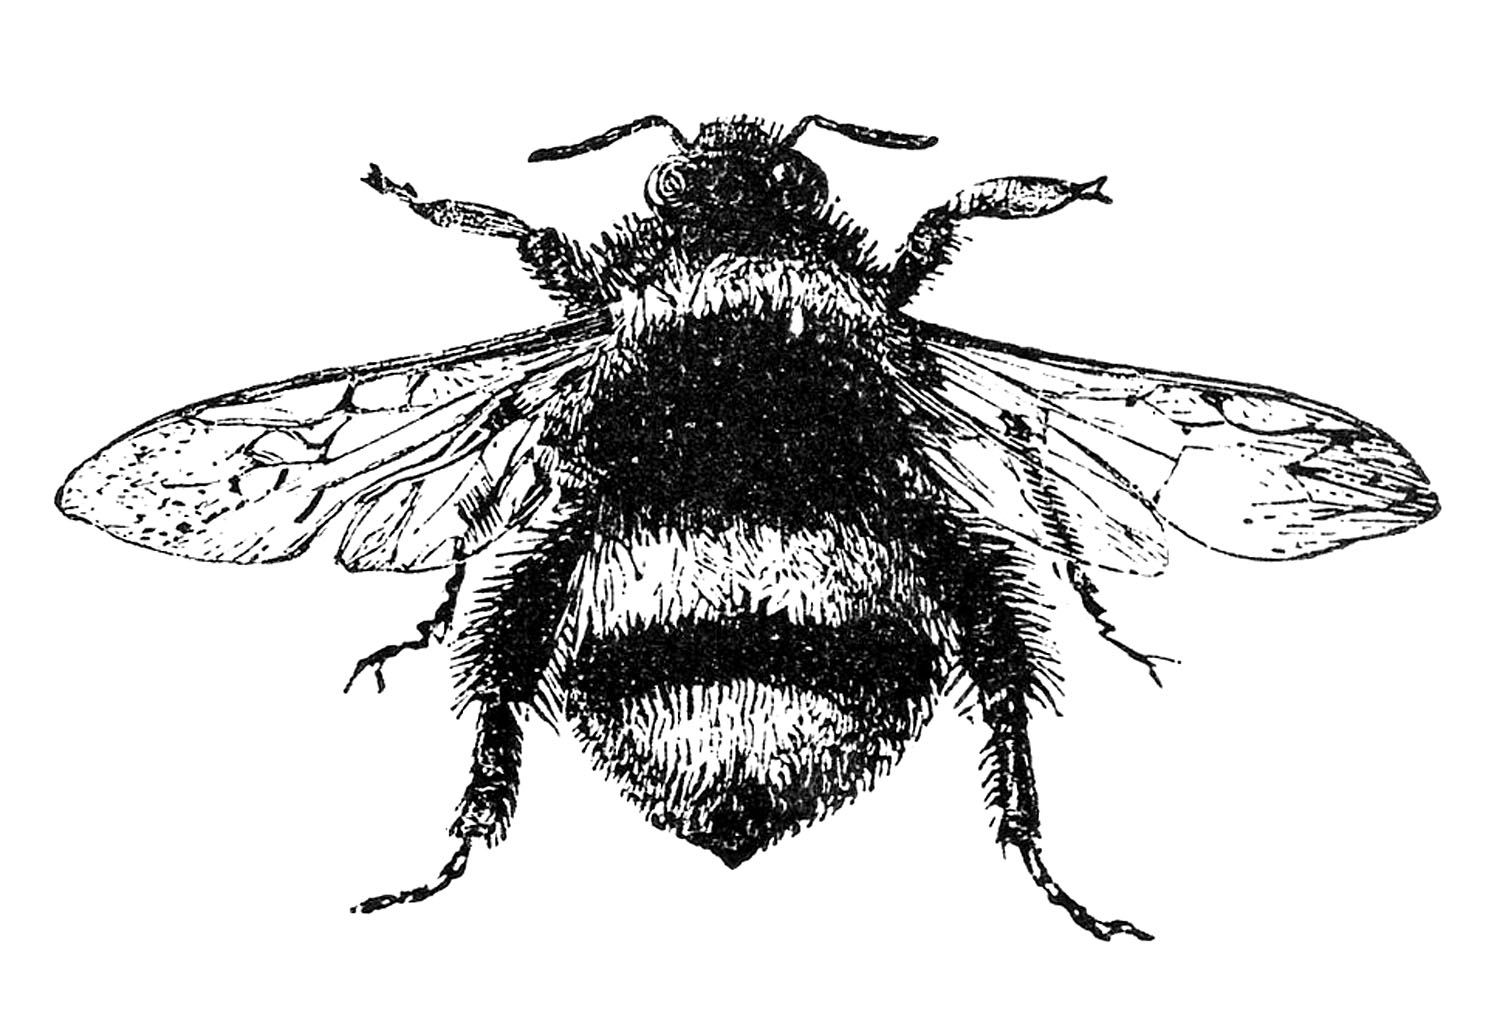
\includegraphics[scale=0.75]{img/bumblebee.jpg}
		\end{figure}
		\vspace{0.5cm}
		\Huge
		\textbf{\textsc{Metody Probabilistyczne Informatyki}}

		\vspace{0.5cm}
		\Large
		\textsc{Wybrane Dowody}

		\normalsize


		\line(1,0){330}

		\vspace{1cm}
		\textit{,,Tak teraz na to patrzę i myślę, czy ta nierówność nie powinna być w drugą stronę...''}
		\vspace{1cm}

		\textit{\textsc{Popełnione przez}}\\
		\vspace{5mm}

		\textbf{\textsc{
				Załatany Ponton \\
				V\\
				Nahtamatu\\
			}}

		\vfill

		Kraków \\
		Anno Domini 2025

	\end{center}

\end{titlepage}


\tableofcontents
\section*{Licencja}
\begin{figure}[h]
	\begin{minipage}[c]{0.25\textwidth}
		
\includegraphics[width=0.7\textwidth]{img/licencja.png}
	\end{minipage}\hfill
	\begin{minipage}[c]{0.75\textwidth}
		\caption*{
			Ten utwór jest dostępny na
			\href{https://creativecommons.org/licenses/by-sa/4.0/}{licencji Creative Commons Uznanie autorstwa
				na tych samych warunkach 4.0 Międzynarodowe.}
		}
	\end{minipage}
\end{figure}

% Remove the "Rozdział x" chapter headings, as we already number our chapters
\titleformat{\chapter}[display]{\normalfont\Huge\bfseries}{}{0pt}{\Huge}
\titlespacing*{\chapter}{0pt}{0pt}{20pt}

% Actual content
\mainmatter

\chapter{Wykład 1 (2025-10-03)}
 % Żeby nie było syfu to kolejne sekcje dodajemy do chapters/
% A potem includujemy za pomocą \input{chapters/...}

% Używamy \( \) i \[ \] zamiast dolarów -- tak jak się robi w LaTeXu


\documentclass[12pt, a4paper, polish, openany]{book}

% Please, let's familiarize ourselves with notatki.sty and tcs.sty so that we don't reinvent the wheel
\usepackage{notatki}
\fancyhead[L]{\textbf{\textit{MPI}}}

\begin{document}
% Front page and table of contents
\frontmatter

\input{titlepage}

\tableofcontents
\input{license}

% Remove the "Rozdział x" chapter headings, as we already number our chapters
\titleformat{\chapter}[display]{\normalfont\Huge\bfseries}{}{0pt}{\Huge}
\titlespacing*{\chapter}{0pt}{0pt}{20pt}

% Actual content
\mainmatter

\chapter{Wykład 1 (2025-10-03)}
\input{chapters/2025-10-03-lecture/main}

\chapter{Nagranie 1 (2025-10-04)}
\input{chapters/2025-10-04-recording/main}

\chapter{Wykład 2 (2025-10-10)}
\input{chapters/2025-10-10-lecture/main}

\chapter{Nagranie 2 (2025-10-10)}
\input{chapters/2025-10-10-recording/main}

\chapter{Wykład 3 (2025-10-17)}
\input{chapters/2025-10-17-lecture/main}

\end{document}


\chapter{Nagranie 1 (2025-10-04)}
 % Żeby nie było syfu to kolejne sekcje dodajemy do chapters/
% A potem includujemy za pomocą \input{chapters/...}

% Używamy \( \) i \[ \] zamiast dolarów -- tak jak się robi w LaTeXu


\documentclass[12pt, a4paper, polish, openany]{book}

% Please, let's familiarize ourselves with notatki.sty and tcs.sty so that we don't reinvent the wheel
\usepackage{notatki}
\fancyhead[L]{\textbf{\textit{MPI}}}

\begin{document}
% Front page and table of contents
\frontmatter

\input{titlepage}

\tableofcontents
\input{license}

% Remove the "Rozdział x" chapter headings, as we already number our chapters
\titleformat{\chapter}[display]{\normalfont\Huge\bfseries}{}{0pt}{\Huge}
\titlespacing*{\chapter}{0pt}{0pt}{20pt}

% Actual content
\mainmatter

\chapter{Wykład 1 (2025-10-03)}
\input{chapters/2025-10-03-lecture/main}

\chapter{Nagranie 1 (2025-10-04)}
\input{chapters/2025-10-04-recording/main}

\chapter{Wykład 2 (2025-10-10)}
\input{chapters/2025-10-10-lecture/main}

\chapter{Nagranie 2 (2025-10-10)}
\input{chapters/2025-10-10-recording/main}

\chapter{Wykład 3 (2025-10-17)}
\input{chapters/2025-10-17-lecture/main}

\end{document}


\chapter{Wykład 2 (2025-10-10)}
 % Żeby nie było syfu to kolejne sekcje dodajemy do chapters/
% A potem includujemy za pomocą \input{chapters/...}

% Używamy \( \) i \[ \] zamiast dolarów -- tak jak się robi w LaTeXu


\documentclass[12pt, a4paper, polish, openany]{book}

% Please, let's familiarize ourselves with notatki.sty and tcs.sty so that we don't reinvent the wheel
\usepackage{notatki}
\fancyhead[L]{\textbf{\textit{MPI}}}

\begin{document}
% Front page and table of contents
\frontmatter

\input{titlepage}

\tableofcontents
\input{license}

% Remove the "Rozdział x" chapter headings, as we already number our chapters
\titleformat{\chapter}[display]{\normalfont\Huge\bfseries}{}{0pt}{\Huge}
\titlespacing*{\chapter}{0pt}{0pt}{20pt}

% Actual content
\mainmatter

\chapter{Wykład 1 (2025-10-03)}
\input{chapters/2025-10-03-lecture/main}

\chapter{Nagranie 1 (2025-10-04)}
\input{chapters/2025-10-04-recording/main}

\chapter{Wykład 2 (2025-10-10)}
\input{chapters/2025-10-10-lecture/main}

\chapter{Nagranie 2 (2025-10-10)}
\input{chapters/2025-10-10-recording/main}

\chapter{Wykład 3 (2025-10-17)}
\input{chapters/2025-10-17-lecture/main}

\end{document}


\chapter{Nagranie 2 (2025-10-10)}
 % Żeby nie było syfu to kolejne sekcje dodajemy do chapters/
% A potem includujemy za pomocą \input{chapters/...}

% Używamy \( \) i \[ \] zamiast dolarów -- tak jak się robi w LaTeXu


\documentclass[12pt, a4paper, polish, openany]{book}

% Please, let's familiarize ourselves with notatki.sty and tcs.sty so that we don't reinvent the wheel
\usepackage{notatki}
\fancyhead[L]{\textbf{\textit{MPI}}}

\begin{document}
% Front page and table of contents
\frontmatter

\input{titlepage}

\tableofcontents
\input{license}

% Remove the "Rozdział x" chapter headings, as we already number our chapters
\titleformat{\chapter}[display]{\normalfont\Huge\bfseries}{}{0pt}{\Huge}
\titlespacing*{\chapter}{0pt}{0pt}{20pt}

% Actual content
\mainmatter

\chapter{Wykład 1 (2025-10-03)}
\input{chapters/2025-10-03-lecture/main}

\chapter{Nagranie 1 (2025-10-04)}
\input{chapters/2025-10-04-recording/main}

\chapter{Wykład 2 (2025-10-10)}
\input{chapters/2025-10-10-lecture/main}

\chapter{Nagranie 2 (2025-10-10)}
\input{chapters/2025-10-10-recording/main}

\chapter{Wykład 3 (2025-10-17)}
\input{chapters/2025-10-17-lecture/main}

\end{document}


\chapter{Wykład 3 (2025-10-17)}
 % Żeby nie było syfu to kolejne sekcje dodajemy do chapters/
% A potem includujemy za pomocą \input{chapters/...}

% Używamy \( \) i \[ \] zamiast dolarów -- tak jak się robi w LaTeXu


\documentclass[12pt, a4paper, polish, openany]{book}

% Please, let's familiarize ourselves with notatki.sty and tcs.sty so that we don't reinvent the wheel
\usepackage{notatki}
\fancyhead[L]{\textbf{\textit{MPI}}}

\begin{document}
% Front page and table of contents
\frontmatter

\input{titlepage}

\tableofcontents
\input{license}

% Remove the "Rozdział x" chapter headings, as we already number our chapters
\titleformat{\chapter}[display]{\normalfont\Huge\bfseries}{}{0pt}{\Huge}
\titlespacing*{\chapter}{0pt}{0pt}{20pt}

% Actual content
\mainmatter

\chapter{Wykład 1 (2025-10-03)}
\input{chapters/2025-10-03-lecture/main}

\chapter{Nagranie 1 (2025-10-04)}
\input{chapters/2025-10-04-recording/main}

\chapter{Wykład 2 (2025-10-10)}
\input{chapters/2025-10-10-lecture/main}

\chapter{Nagranie 2 (2025-10-10)}
\input{chapters/2025-10-10-recording/main}

\chapter{Wykład 3 (2025-10-17)}
\input{chapters/2025-10-17-lecture/main}

\end{document}


\end{document}


\chapter{Wykład 3 (2025-10-17)}
 % Żeby nie było syfu to kolejne sekcje dodajemy do chapters/
% A potem includujemy za pomocą \input{chapters/...}

% Używamy \( \) i \[ \] zamiast dolarów -- tak jak się robi w LaTeXu


\documentclass[12pt, a4paper, polish, openany]{book}

% Please, let's familiarize ourselves with notatki.sty and tcs.sty so that we don't reinvent the wheel
\usepackage{notatki}
\fancyhead[L]{\textbf{\textit{MPI}}}

\begin{document}
% Front page and table of contents
\frontmatter

\begin{titlepage}

	\begin{center}
		\begin{figure}[h]
			\centering
			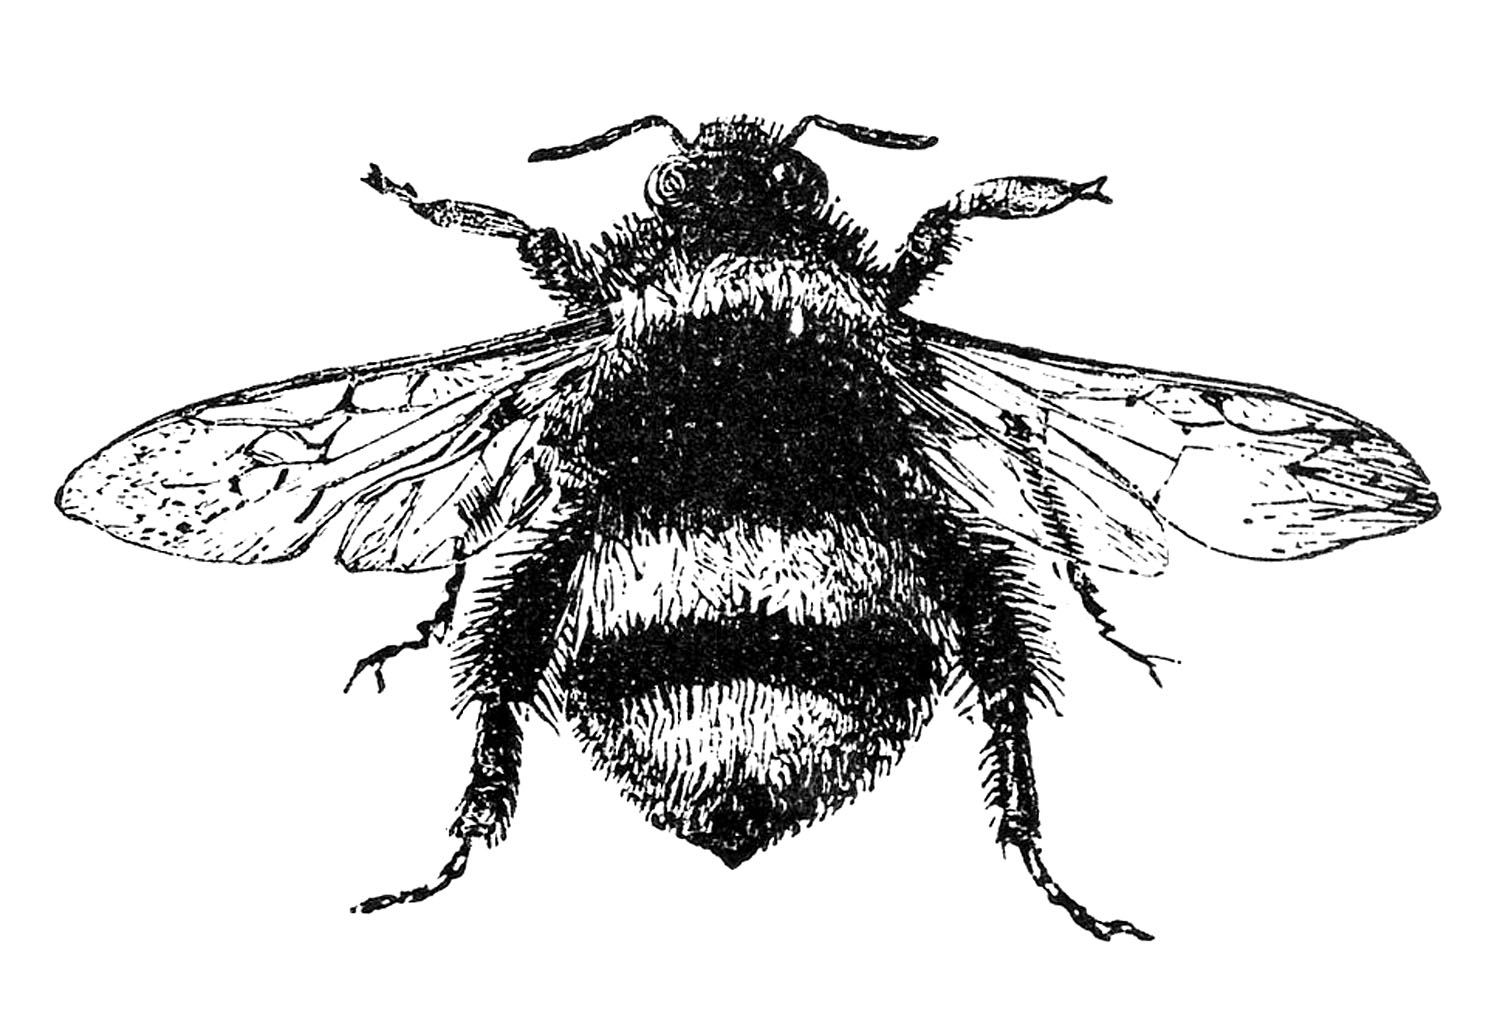
\includegraphics[scale=0.75]{img/bumblebee.jpg}
		\end{figure}
		\vspace{0.5cm}
		\Huge
		\textbf{\textsc{Metody Probabilistyczne Informatyki}}

		\vspace{0.5cm}
		\Large
		\textsc{Wybrane Dowody}

		\normalsize


		\line(1,0){330}

		\vspace{1cm}
		\textit{,,Tak teraz na to patrzę i myślę, czy ta nierówność nie powinna być w drugą stronę...''}
		\vspace{1cm}

		\textit{\textsc{Popełnione przez}}\\
		\vspace{5mm}

		\textbf{\textsc{
				Załatany Ponton \\
				V\\
				Nahtamatu\\
			}}

		\vfill

		Kraków \\
		Anno Domini 2025

	\end{center}

\end{titlepage}


\tableofcontents
\section*{Licencja}
\begin{figure}[h]
	\begin{minipage}[c]{0.25\textwidth}
		
\includegraphics[width=0.7\textwidth]{img/licencja.png}
	\end{minipage}\hfill
	\begin{minipage}[c]{0.75\textwidth}
		\caption*{
			Ten utwór jest dostępny na
			\href{https://creativecommons.org/licenses/by-sa/4.0/}{licencji Creative Commons Uznanie autorstwa
				na tych samych warunkach 4.0 Międzynarodowe.}
		}
	\end{minipage}
\end{figure}

% Remove the "Rozdział x" chapter headings, as we already number our chapters
\titleformat{\chapter}[display]{\normalfont\Huge\bfseries}{}{0pt}{\Huge}
\titlespacing*{\chapter}{0pt}{0pt}{20pt}

% Actual content
\mainmatter

\chapter{Wykład 1 (2025-10-03)}
 % Żeby nie było syfu to kolejne sekcje dodajemy do chapters/
% A potem includujemy za pomocą \input{chapters/...}

% Używamy \( \) i \[ \] zamiast dolarów -- tak jak się robi w LaTeXu


\documentclass[12pt, a4paper, polish, openany]{book}

% Please, let's familiarize ourselves with notatki.sty and tcs.sty so that we don't reinvent the wheel
\usepackage{notatki}
\fancyhead[L]{\textbf{\textit{MPI}}}

\begin{document}
% Front page and table of contents
\frontmatter

\input{titlepage}

\tableofcontents
\input{license}

% Remove the "Rozdział x" chapter headings, as we already number our chapters
\titleformat{\chapter}[display]{\normalfont\Huge\bfseries}{}{0pt}{\Huge}
\titlespacing*{\chapter}{0pt}{0pt}{20pt}

% Actual content
\mainmatter

\chapter{Wykład 1 (2025-10-03)}
\input{chapters/2025-10-03-lecture/main}

\chapter{Nagranie 1 (2025-10-04)}
\input{chapters/2025-10-04-recording/main}

\chapter{Wykład 2 (2025-10-10)}
\input{chapters/2025-10-10-lecture/main}

\chapter{Nagranie 2 (2025-10-10)}
\input{chapters/2025-10-10-recording/main}

\chapter{Wykład 3 (2025-10-17)}
\input{chapters/2025-10-17-lecture/main}

\end{document}


\chapter{Nagranie 1 (2025-10-04)}
 % Żeby nie było syfu to kolejne sekcje dodajemy do chapters/
% A potem includujemy za pomocą \input{chapters/...}

% Używamy \( \) i \[ \] zamiast dolarów -- tak jak się robi w LaTeXu


\documentclass[12pt, a4paper, polish, openany]{book}

% Please, let's familiarize ourselves with notatki.sty and tcs.sty so that we don't reinvent the wheel
\usepackage{notatki}
\fancyhead[L]{\textbf{\textit{MPI}}}

\begin{document}
% Front page and table of contents
\frontmatter

\input{titlepage}

\tableofcontents
\input{license}

% Remove the "Rozdział x" chapter headings, as we already number our chapters
\titleformat{\chapter}[display]{\normalfont\Huge\bfseries}{}{0pt}{\Huge}
\titlespacing*{\chapter}{0pt}{0pt}{20pt}

% Actual content
\mainmatter

\chapter{Wykład 1 (2025-10-03)}
\input{chapters/2025-10-03-lecture/main}

\chapter{Nagranie 1 (2025-10-04)}
\input{chapters/2025-10-04-recording/main}

\chapter{Wykład 2 (2025-10-10)}
\input{chapters/2025-10-10-lecture/main}

\chapter{Nagranie 2 (2025-10-10)}
\input{chapters/2025-10-10-recording/main}

\chapter{Wykład 3 (2025-10-17)}
\input{chapters/2025-10-17-lecture/main}

\end{document}


\chapter{Wykład 2 (2025-10-10)}
 % Żeby nie było syfu to kolejne sekcje dodajemy do chapters/
% A potem includujemy za pomocą \input{chapters/...}

% Używamy \( \) i \[ \] zamiast dolarów -- tak jak się robi w LaTeXu


\documentclass[12pt, a4paper, polish, openany]{book}

% Please, let's familiarize ourselves with notatki.sty and tcs.sty so that we don't reinvent the wheel
\usepackage{notatki}
\fancyhead[L]{\textbf{\textit{MPI}}}

\begin{document}
% Front page and table of contents
\frontmatter

\input{titlepage}

\tableofcontents
\input{license}

% Remove the "Rozdział x" chapter headings, as we already number our chapters
\titleformat{\chapter}[display]{\normalfont\Huge\bfseries}{}{0pt}{\Huge}
\titlespacing*{\chapter}{0pt}{0pt}{20pt}

% Actual content
\mainmatter

\chapter{Wykład 1 (2025-10-03)}
\input{chapters/2025-10-03-lecture/main}

\chapter{Nagranie 1 (2025-10-04)}
\input{chapters/2025-10-04-recording/main}

\chapter{Wykład 2 (2025-10-10)}
\input{chapters/2025-10-10-lecture/main}

\chapter{Nagranie 2 (2025-10-10)}
\input{chapters/2025-10-10-recording/main}

\chapter{Wykład 3 (2025-10-17)}
\input{chapters/2025-10-17-lecture/main}

\end{document}


\chapter{Nagranie 2 (2025-10-10)}
 % Żeby nie było syfu to kolejne sekcje dodajemy do chapters/
% A potem includujemy za pomocą \input{chapters/...}

% Używamy \( \) i \[ \] zamiast dolarów -- tak jak się robi w LaTeXu


\documentclass[12pt, a4paper, polish, openany]{book}

% Please, let's familiarize ourselves with notatki.sty and tcs.sty so that we don't reinvent the wheel
\usepackage{notatki}
\fancyhead[L]{\textbf{\textit{MPI}}}

\begin{document}
% Front page and table of contents
\frontmatter

\input{titlepage}

\tableofcontents
\input{license}

% Remove the "Rozdział x" chapter headings, as we already number our chapters
\titleformat{\chapter}[display]{\normalfont\Huge\bfseries}{}{0pt}{\Huge}
\titlespacing*{\chapter}{0pt}{0pt}{20pt}

% Actual content
\mainmatter

\chapter{Wykład 1 (2025-10-03)}
\input{chapters/2025-10-03-lecture/main}

\chapter{Nagranie 1 (2025-10-04)}
\input{chapters/2025-10-04-recording/main}

\chapter{Wykład 2 (2025-10-10)}
\input{chapters/2025-10-10-lecture/main}

\chapter{Nagranie 2 (2025-10-10)}
\input{chapters/2025-10-10-recording/main}

\chapter{Wykład 3 (2025-10-17)}
\input{chapters/2025-10-17-lecture/main}

\end{document}


\chapter{Wykład 3 (2025-10-17)}
 % Żeby nie było syfu to kolejne sekcje dodajemy do chapters/
% A potem includujemy za pomocą \input{chapters/...}

% Używamy \( \) i \[ \] zamiast dolarów -- tak jak się robi w LaTeXu


\documentclass[12pt, a4paper, polish, openany]{book}

% Please, let's familiarize ourselves with notatki.sty and tcs.sty so that we don't reinvent the wheel
\usepackage{notatki}
\fancyhead[L]{\textbf{\textit{MPI}}}

\begin{document}
% Front page and table of contents
\frontmatter

\input{titlepage}

\tableofcontents
\input{license}

% Remove the "Rozdział x" chapter headings, as we already number our chapters
\titleformat{\chapter}[display]{\normalfont\Huge\bfseries}{}{0pt}{\Huge}
\titlespacing*{\chapter}{0pt}{0pt}{20pt}

% Actual content
\mainmatter

\chapter{Wykład 1 (2025-10-03)}
\input{chapters/2025-10-03-lecture/main}

\chapter{Nagranie 1 (2025-10-04)}
\input{chapters/2025-10-04-recording/main}

\chapter{Wykład 2 (2025-10-10)}
\input{chapters/2025-10-10-lecture/main}

\chapter{Nagranie 2 (2025-10-10)}
\input{chapters/2025-10-10-recording/main}

\chapter{Wykład 3 (2025-10-17)}
\input{chapters/2025-10-17-lecture/main}

\end{document}


\end{document}


\end{document}


\realsection{Porządki częściowe, Twierdzenia Dilwortha i Spernera}
 % Żeby nie było syfu to kolejne sekcje dodajemy do chapters/
% A potem includujemy za pomocą \input{chapters/...}

% Używamy \( \) i \[ \] zamiast dolarów -- tak jak się robi w LaTeXu


\documentclass[12pt, a4paper, polish, openany]{book}

% Please, let's familiarize ourselves with notatki.sty and tcs.sty so that we don't reinvent the wheel
\usepackage{notatki}
\fancyhead[L]{\textbf{\textit{MPI}}}

\begin{document}
% Front page and table of contents
\frontmatter

\begin{titlepage}

	\begin{center}
		\begin{figure}[h]
			\centering
			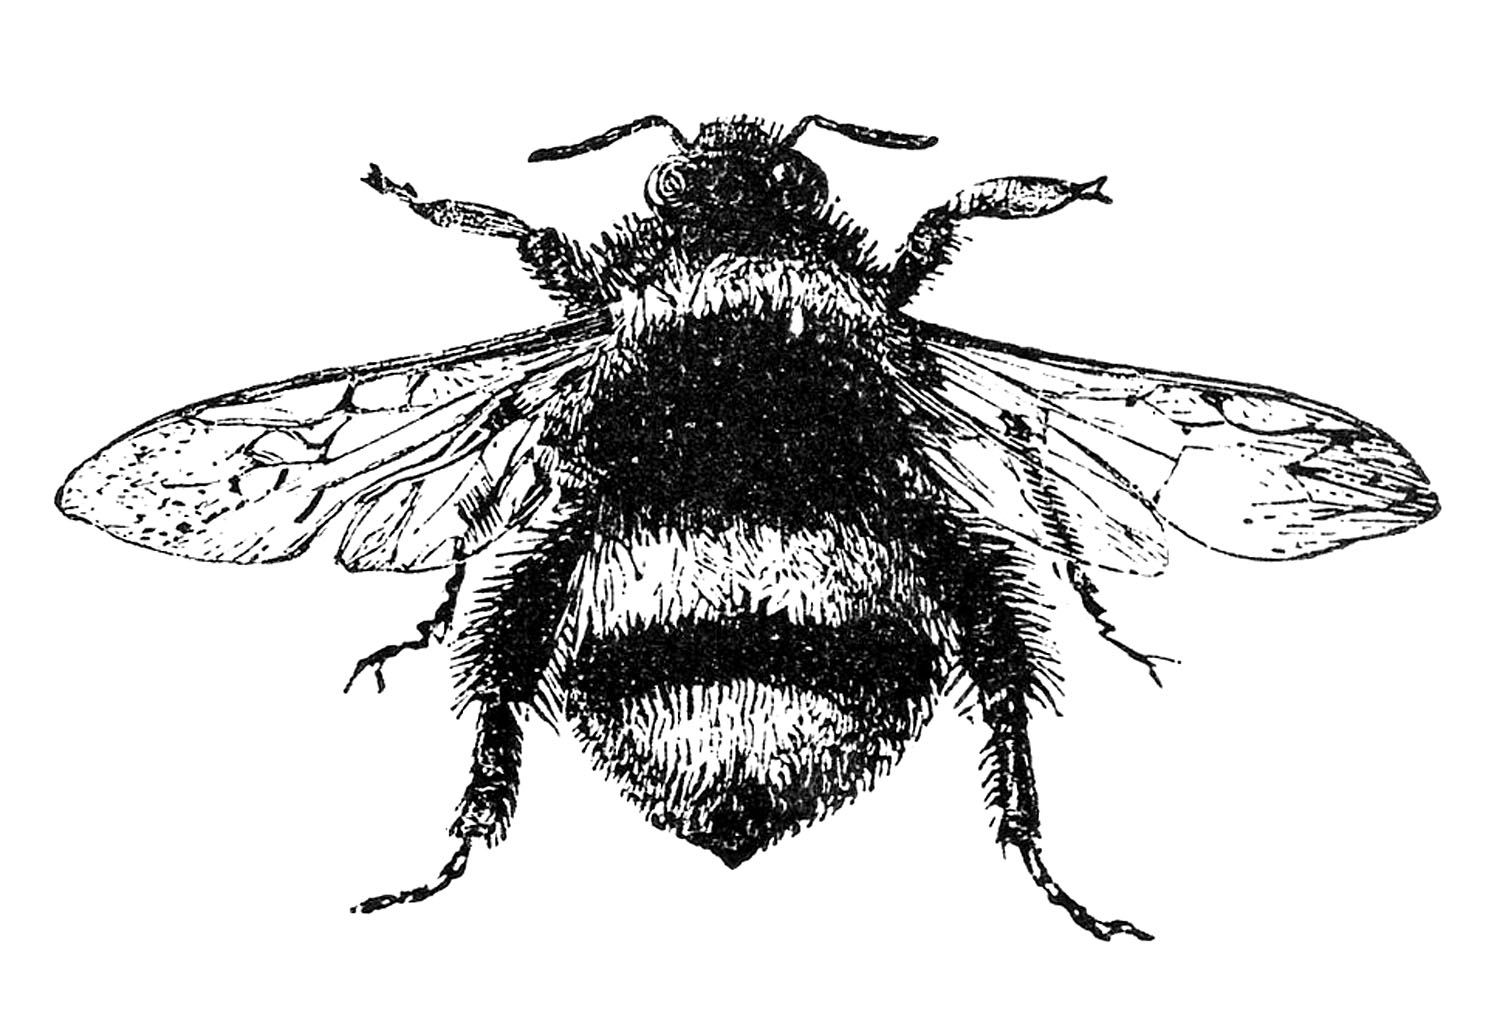
\includegraphics[scale=0.75]{img/bumblebee.jpg}
		\end{figure}
		\vspace{0.5cm}
		\Huge
		\textbf{\textsc{Metody Probabilistyczne Informatyki}}

		\vspace{0.5cm}
		\Large
		\textsc{Wybrane Dowody}

		\normalsize


		\line(1,0){330}

		\vspace{1cm}
		\textit{,,Tak teraz na to patrzę i myślę, czy ta nierówność nie powinna być w drugą stronę...''}
		\vspace{1cm}

		\textit{\textsc{Popełnione przez}}\\
		\vspace{5mm}

		\textbf{\textsc{
				Załatany Ponton \\
				V\\
				Nahtamatu\\
			}}

		\vfill

		Kraków \\
		Anno Domini 2025

	\end{center}

\end{titlepage}


\tableofcontents
\section*{Licencja}
\begin{figure}[h]
	\begin{minipage}[c]{0.25\textwidth}
		
\includegraphics[width=0.7\textwidth]{img/licencja.png}
	\end{minipage}\hfill
	\begin{minipage}[c]{0.75\textwidth}
		\caption*{
			Ten utwór jest dostępny na
			\href{https://creativecommons.org/licenses/by-sa/4.0/}{licencji Creative Commons Uznanie autorstwa
				na tych samych warunkach 4.0 Międzynarodowe.}
		}
	\end{minipage}
\end{figure}

% Remove the "Rozdział x" chapter headings, as we already number our chapters
\titleformat{\chapter}[display]{\normalfont\Huge\bfseries}{}{0pt}{\Huge}
\titlespacing*{\chapter}{0pt}{0pt}{20pt}

% Actual content
\mainmatter

\chapter{Wykład 1 (2025-10-03)}
 % Żeby nie było syfu to kolejne sekcje dodajemy do chapters/
% A potem includujemy za pomocą \input{chapters/...}

% Używamy \( \) i \[ \] zamiast dolarów -- tak jak się robi w LaTeXu


\documentclass[12pt, a4paper, polish, openany]{book}

% Please, let's familiarize ourselves with notatki.sty and tcs.sty so that we don't reinvent the wheel
\usepackage{notatki}
\fancyhead[L]{\textbf{\textit{MPI}}}

\begin{document}
% Front page and table of contents
\frontmatter

\begin{titlepage}

	\begin{center}
		\begin{figure}[h]
			\centering
			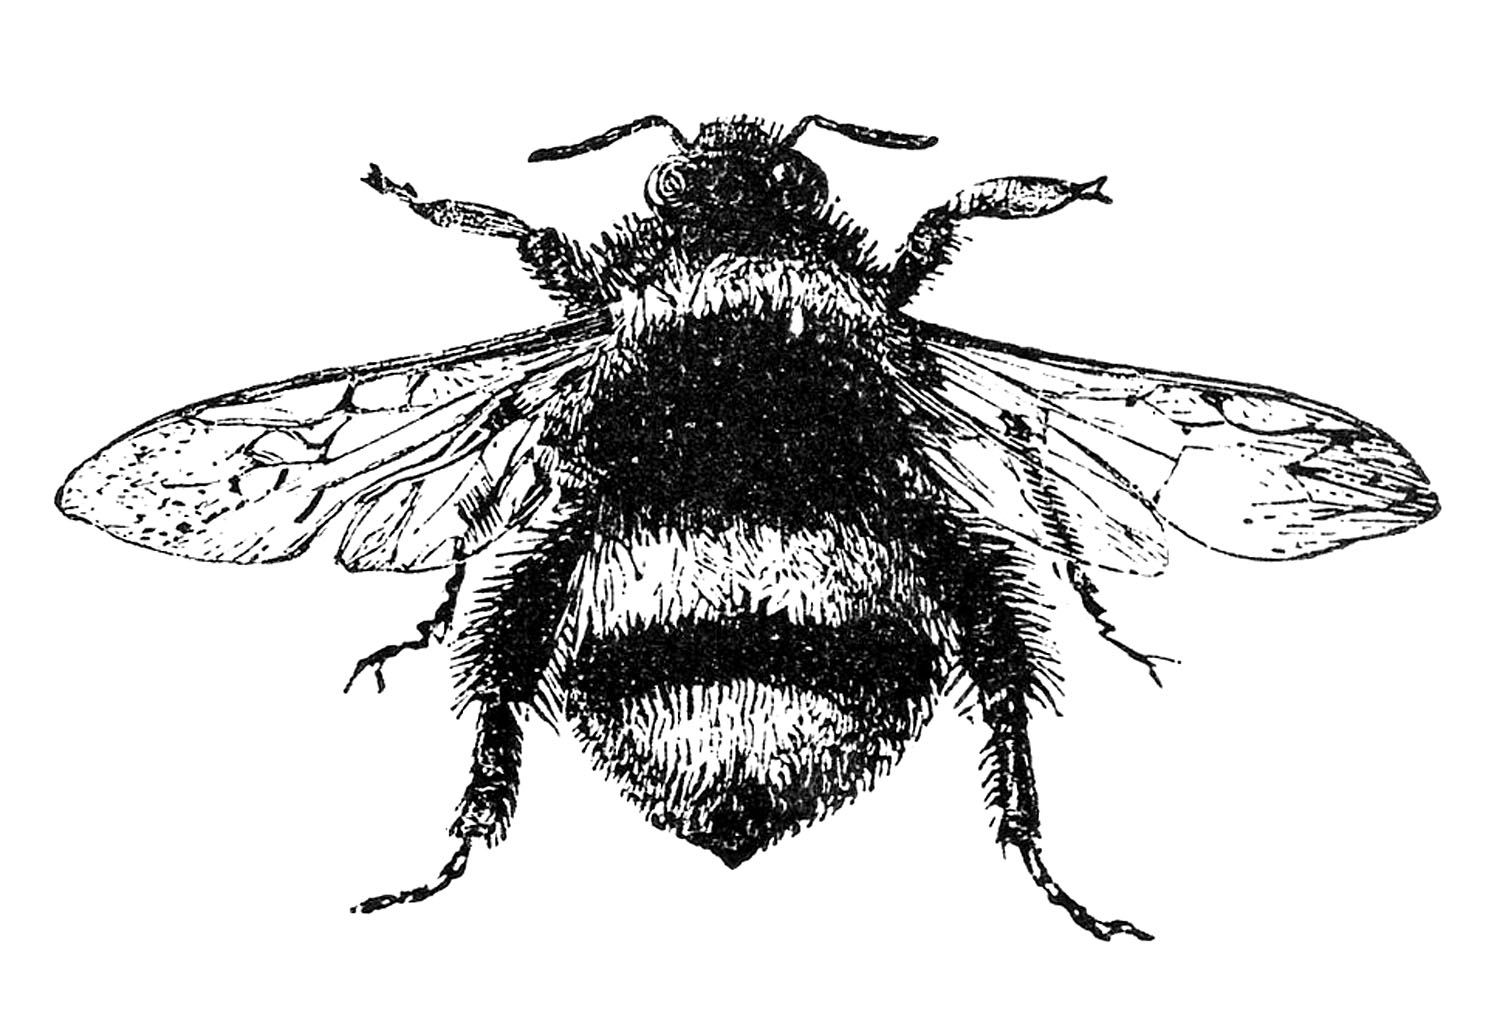
\includegraphics[scale=0.75]{img/bumblebee.jpg}
		\end{figure}
		\vspace{0.5cm}
		\Huge
		\textbf{\textsc{Metody Probabilistyczne Informatyki}}

		\vspace{0.5cm}
		\Large
		\textsc{Wybrane Dowody}

		\normalsize


		\line(1,0){330}

		\vspace{1cm}
		\textit{,,Tak teraz na to patrzę i myślę, czy ta nierówność nie powinna być w drugą stronę...''}
		\vspace{1cm}

		\textit{\textsc{Popełnione przez}}\\
		\vspace{5mm}

		\textbf{\textsc{
				Załatany Ponton \\
				V\\
				Nahtamatu\\
			}}

		\vfill

		Kraków \\
		Anno Domini 2025

	\end{center}

\end{titlepage}


\tableofcontents
\section*{Licencja}
\begin{figure}[h]
	\begin{minipage}[c]{0.25\textwidth}
		
\includegraphics[width=0.7\textwidth]{img/licencja.png}
	\end{minipage}\hfill
	\begin{minipage}[c]{0.75\textwidth}
		\caption*{
			Ten utwór jest dostępny na
			\href{https://creativecommons.org/licenses/by-sa/4.0/}{licencji Creative Commons Uznanie autorstwa
				na tych samych warunkach 4.0 Międzynarodowe.}
		}
	\end{minipage}
\end{figure}

% Remove the "Rozdział x" chapter headings, as we already number our chapters
\titleformat{\chapter}[display]{\normalfont\Huge\bfseries}{}{0pt}{\Huge}
\titlespacing*{\chapter}{0pt}{0pt}{20pt}

% Actual content
\mainmatter

\chapter{Wykład 1 (2025-10-03)}
 % Żeby nie było syfu to kolejne sekcje dodajemy do chapters/
% A potem includujemy za pomocą \input{chapters/...}

% Używamy \( \) i \[ \] zamiast dolarów -- tak jak się robi w LaTeXu


\documentclass[12pt, a4paper, polish, openany]{book}

% Please, let's familiarize ourselves with notatki.sty and tcs.sty so that we don't reinvent the wheel
\usepackage{notatki}
\fancyhead[L]{\textbf{\textit{MPI}}}

\begin{document}
% Front page and table of contents
\frontmatter

\input{titlepage}

\tableofcontents
\input{license}

% Remove the "Rozdział x" chapter headings, as we already number our chapters
\titleformat{\chapter}[display]{\normalfont\Huge\bfseries}{}{0pt}{\Huge}
\titlespacing*{\chapter}{0pt}{0pt}{20pt}

% Actual content
\mainmatter

\chapter{Wykład 1 (2025-10-03)}
\input{chapters/2025-10-03-lecture/main}

\chapter{Nagranie 1 (2025-10-04)}
\input{chapters/2025-10-04-recording/main}

\chapter{Wykład 2 (2025-10-10)}
\input{chapters/2025-10-10-lecture/main}

\chapter{Nagranie 2 (2025-10-10)}
\input{chapters/2025-10-10-recording/main}

\chapter{Wykład 3 (2025-10-17)}
\input{chapters/2025-10-17-lecture/main}

\end{document}


\chapter{Nagranie 1 (2025-10-04)}
 % Żeby nie było syfu to kolejne sekcje dodajemy do chapters/
% A potem includujemy za pomocą \input{chapters/...}

% Używamy \( \) i \[ \] zamiast dolarów -- tak jak się robi w LaTeXu


\documentclass[12pt, a4paper, polish, openany]{book}

% Please, let's familiarize ourselves with notatki.sty and tcs.sty so that we don't reinvent the wheel
\usepackage{notatki}
\fancyhead[L]{\textbf{\textit{MPI}}}

\begin{document}
% Front page and table of contents
\frontmatter

\input{titlepage}

\tableofcontents
\input{license}

% Remove the "Rozdział x" chapter headings, as we already number our chapters
\titleformat{\chapter}[display]{\normalfont\Huge\bfseries}{}{0pt}{\Huge}
\titlespacing*{\chapter}{0pt}{0pt}{20pt}

% Actual content
\mainmatter

\chapter{Wykład 1 (2025-10-03)}
\input{chapters/2025-10-03-lecture/main}

\chapter{Nagranie 1 (2025-10-04)}
\input{chapters/2025-10-04-recording/main}

\chapter{Wykład 2 (2025-10-10)}
\input{chapters/2025-10-10-lecture/main}

\chapter{Nagranie 2 (2025-10-10)}
\input{chapters/2025-10-10-recording/main}

\chapter{Wykład 3 (2025-10-17)}
\input{chapters/2025-10-17-lecture/main}

\end{document}


\chapter{Wykład 2 (2025-10-10)}
 % Żeby nie było syfu to kolejne sekcje dodajemy do chapters/
% A potem includujemy za pomocą \input{chapters/...}

% Używamy \( \) i \[ \] zamiast dolarów -- tak jak się robi w LaTeXu


\documentclass[12pt, a4paper, polish, openany]{book}

% Please, let's familiarize ourselves with notatki.sty and tcs.sty so that we don't reinvent the wheel
\usepackage{notatki}
\fancyhead[L]{\textbf{\textit{MPI}}}

\begin{document}
% Front page and table of contents
\frontmatter

\input{titlepage}

\tableofcontents
\input{license}

% Remove the "Rozdział x" chapter headings, as we already number our chapters
\titleformat{\chapter}[display]{\normalfont\Huge\bfseries}{}{0pt}{\Huge}
\titlespacing*{\chapter}{0pt}{0pt}{20pt}

% Actual content
\mainmatter

\chapter{Wykład 1 (2025-10-03)}
\input{chapters/2025-10-03-lecture/main}

\chapter{Nagranie 1 (2025-10-04)}
\input{chapters/2025-10-04-recording/main}

\chapter{Wykład 2 (2025-10-10)}
\input{chapters/2025-10-10-lecture/main}

\chapter{Nagranie 2 (2025-10-10)}
\input{chapters/2025-10-10-recording/main}

\chapter{Wykład 3 (2025-10-17)}
\input{chapters/2025-10-17-lecture/main}

\end{document}


\chapter{Nagranie 2 (2025-10-10)}
 % Żeby nie było syfu to kolejne sekcje dodajemy do chapters/
% A potem includujemy za pomocą \input{chapters/...}

% Używamy \( \) i \[ \] zamiast dolarów -- tak jak się robi w LaTeXu


\documentclass[12pt, a4paper, polish, openany]{book}

% Please, let's familiarize ourselves with notatki.sty and tcs.sty so that we don't reinvent the wheel
\usepackage{notatki}
\fancyhead[L]{\textbf{\textit{MPI}}}

\begin{document}
% Front page and table of contents
\frontmatter

\input{titlepage}

\tableofcontents
\input{license}

% Remove the "Rozdział x" chapter headings, as we already number our chapters
\titleformat{\chapter}[display]{\normalfont\Huge\bfseries}{}{0pt}{\Huge}
\titlespacing*{\chapter}{0pt}{0pt}{20pt}

% Actual content
\mainmatter

\chapter{Wykład 1 (2025-10-03)}
\input{chapters/2025-10-03-lecture/main}

\chapter{Nagranie 1 (2025-10-04)}
\input{chapters/2025-10-04-recording/main}

\chapter{Wykład 2 (2025-10-10)}
\input{chapters/2025-10-10-lecture/main}

\chapter{Nagranie 2 (2025-10-10)}
\input{chapters/2025-10-10-recording/main}

\chapter{Wykład 3 (2025-10-17)}
\input{chapters/2025-10-17-lecture/main}

\end{document}


\chapter{Wykład 3 (2025-10-17)}
 % Żeby nie było syfu to kolejne sekcje dodajemy do chapters/
% A potem includujemy za pomocą \input{chapters/...}

% Używamy \( \) i \[ \] zamiast dolarów -- tak jak się robi w LaTeXu


\documentclass[12pt, a4paper, polish, openany]{book}

% Please, let's familiarize ourselves with notatki.sty and tcs.sty so that we don't reinvent the wheel
\usepackage{notatki}
\fancyhead[L]{\textbf{\textit{MPI}}}

\begin{document}
% Front page and table of contents
\frontmatter

\input{titlepage}

\tableofcontents
\input{license}

% Remove the "Rozdział x" chapter headings, as we already number our chapters
\titleformat{\chapter}[display]{\normalfont\Huge\bfseries}{}{0pt}{\Huge}
\titlespacing*{\chapter}{0pt}{0pt}{20pt}

% Actual content
\mainmatter

\chapter{Wykład 1 (2025-10-03)}
\input{chapters/2025-10-03-lecture/main}

\chapter{Nagranie 1 (2025-10-04)}
\input{chapters/2025-10-04-recording/main}

\chapter{Wykład 2 (2025-10-10)}
\input{chapters/2025-10-10-lecture/main}

\chapter{Nagranie 2 (2025-10-10)}
\input{chapters/2025-10-10-recording/main}

\chapter{Wykład 3 (2025-10-17)}
\input{chapters/2025-10-17-lecture/main}

\end{document}


\end{document}


\chapter{Nagranie 1 (2025-10-04)}
 % Żeby nie było syfu to kolejne sekcje dodajemy do chapters/
% A potem includujemy za pomocą \input{chapters/...}

% Używamy \( \) i \[ \] zamiast dolarów -- tak jak się robi w LaTeXu


\documentclass[12pt, a4paper, polish, openany]{book}

% Please, let's familiarize ourselves with notatki.sty and tcs.sty so that we don't reinvent the wheel
\usepackage{notatki}
\fancyhead[L]{\textbf{\textit{MPI}}}

\begin{document}
% Front page and table of contents
\frontmatter

\begin{titlepage}

	\begin{center}
		\begin{figure}[h]
			\centering
			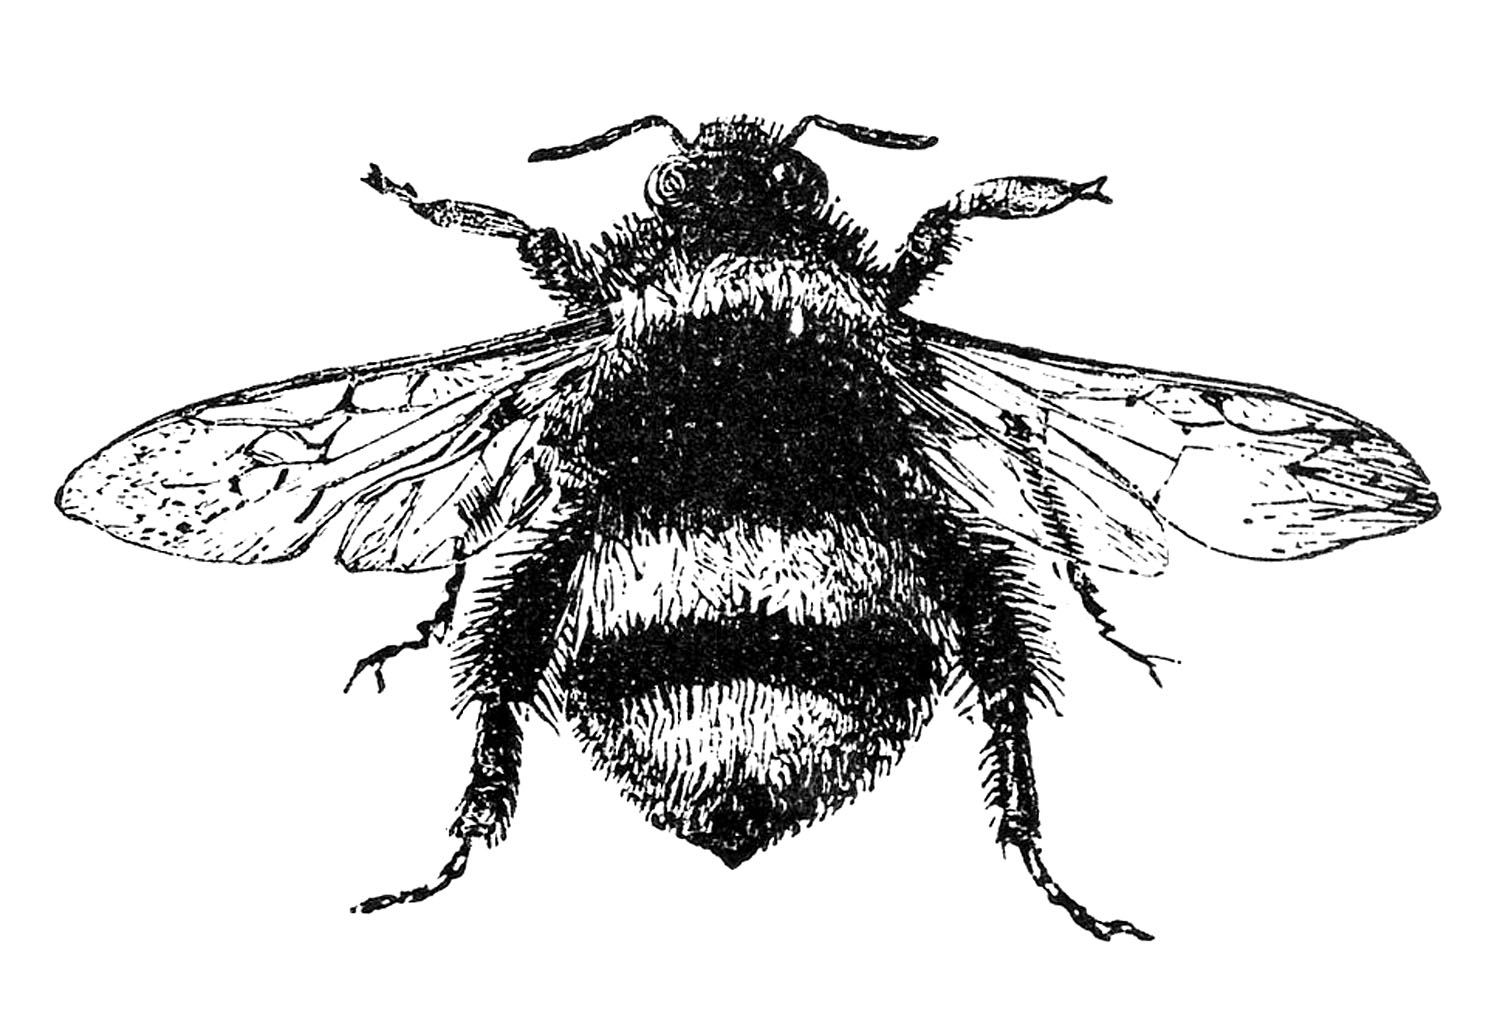
\includegraphics[scale=0.75]{img/bumblebee.jpg}
		\end{figure}
		\vspace{0.5cm}
		\Huge
		\textbf{\textsc{Metody Probabilistyczne Informatyki}}

		\vspace{0.5cm}
		\Large
		\textsc{Wybrane Dowody}

		\normalsize


		\line(1,0){330}

		\vspace{1cm}
		\textit{,,Tak teraz na to patrzę i myślę, czy ta nierówność nie powinna być w drugą stronę...''}
		\vspace{1cm}

		\textit{\textsc{Popełnione przez}}\\
		\vspace{5mm}

		\textbf{\textsc{
				Załatany Ponton \\
				V\\
				Nahtamatu\\
			}}

		\vfill

		Kraków \\
		Anno Domini 2025

	\end{center}

\end{titlepage}


\tableofcontents
\section*{Licencja}
\begin{figure}[h]
	\begin{minipage}[c]{0.25\textwidth}
		
\includegraphics[width=0.7\textwidth]{img/licencja.png}
	\end{minipage}\hfill
	\begin{minipage}[c]{0.75\textwidth}
		\caption*{
			Ten utwór jest dostępny na
			\href{https://creativecommons.org/licenses/by-sa/4.0/}{licencji Creative Commons Uznanie autorstwa
				na tych samych warunkach 4.0 Międzynarodowe.}
		}
	\end{minipage}
\end{figure}

% Remove the "Rozdział x" chapter headings, as we already number our chapters
\titleformat{\chapter}[display]{\normalfont\Huge\bfseries}{}{0pt}{\Huge}
\titlespacing*{\chapter}{0pt}{0pt}{20pt}

% Actual content
\mainmatter

\chapter{Wykład 1 (2025-10-03)}
 % Żeby nie było syfu to kolejne sekcje dodajemy do chapters/
% A potem includujemy za pomocą \input{chapters/...}

% Używamy \( \) i \[ \] zamiast dolarów -- tak jak się robi w LaTeXu


\documentclass[12pt, a4paper, polish, openany]{book}

% Please, let's familiarize ourselves with notatki.sty and tcs.sty so that we don't reinvent the wheel
\usepackage{notatki}
\fancyhead[L]{\textbf{\textit{MPI}}}

\begin{document}
% Front page and table of contents
\frontmatter

\input{titlepage}

\tableofcontents
\input{license}

% Remove the "Rozdział x" chapter headings, as we already number our chapters
\titleformat{\chapter}[display]{\normalfont\Huge\bfseries}{}{0pt}{\Huge}
\titlespacing*{\chapter}{0pt}{0pt}{20pt}

% Actual content
\mainmatter

\chapter{Wykład 1 (2025-10-03)}
\input{chapters/2025-10-03-lecture/main}

\chapter{Nagranie 1 (2025-10-04)}
\input{chapters/2025-10-04-recording/main}

\chapter{Wykład 2 (2025-10-10)}
\input{chapters/2025-10-10-lecture/main}

\chapter{Nagranie 2 (2025-10-10)}
\input{chapters/2025-10-10-recording/main}

\chapter{Wykład 3 (2025-10-17)}
\input{chapters/2025-10-17-lecture/main}

\end{document}


\chapter{Nagranie 1 (2025-10-04)}
 % Żeby nie było syfu to kolejne sekcje dodajemy do chapters/
% A potem includujemy za pomocą \input{chapters/...}

% Używamy \( \) i \[ \] zamiast dolarów -- tak jak się robi w LaTeXu


\documentclass[12pt, a4paper, polish, openany]{book}

% Please, let's familiarize ourselves with notatki.sty and tcs.sty so that we don't reinvent the wheel
\usepackage{notatki}
\fancyhead[L]{\textbf{\textit{MPI}}}

\begin{document}
% Front page and table of contents
\frontmatter

\input{titlepage}

\tableofcontents
\input{license}

% Remove the "Rozdział x" chapter headings, as we already number our chapters
\titleformat{\chapter}[display]{\normalfont\Huge\bfseries}{}{0pt}{\Huge}
\titlespacing*{\chapter}{0pt}{0pt}{20pt}

% Actual content
\mainmatter

\chapter{Wykład 1 (2025-10-03)}
\input{chapters/2025-10-03-lecture/main}

\chapter{Nagranie 1 (2025-10-04)}
\input{chapters/2025-10-04-recording/main}

\chapter{Wykład 2 (2025-10-10)}
\input{chapters/2025-10-10-lecture/main}

\chapter{Nagranie 2 (2025-10-10)}
\input{chapters/2025-10-10-recording/main}

\chapter{Wykład 3 (2025-10-17)}
\input{chapters/2025-10-17-lecture/main}

\end{document}


\chapter{Wykład 2 (2025-10-10)}
 % Żeby nie było syfu to kolejne sekcje dodajemy do chapters/
% A potem includujemy za pomocą \input{chapters/...}

% Używamy \( \) i \[ \] zamiast dolarów -- tak jak się robi w LaTeXu


\documentclass[12pt, a4paper, polish, openany]{book}

% Please, let's familiarize ourselves with notatki.sty and tcs.sty so that we don't reinvent the wheel
\usepackage{notatki}
\fancyhead[L]{\textbf{\textit{MPI}}}

\begin{document}
% Front page and table of contents
\frontmatter

\input{titlepage}

\tableofcontents
\input{license}

% Remove the "Rozdział x" chapter headings, as we already number our chapters
\titleformat{\chapter}[display]{\normalfont\Huge\bfseries}{}{0pt}{\Huge}
\titlespacing*{\chapter}{0pt}{0pt}{20pt}

% Actual content
\mainmatter

\chapter{Wykład 1 (2025-10-03)}
\input{chapters/2025-10-03-lecture/main}

\chapter{Nagranie 1 (2025-10-04)}
\input{chapters/2025-10-04-recording/main}

\chapter{Wykład 2 (2025-10-10)}
\input{chapters/2025-10-10-lecture/main}

\chapter{Nagranie 2 (2025-10-10)}
\input{chapters/2025-10-10-recording/main}

\chapter{Wykład 3 (2025-10-17)}
\input{chapters/2025-10-17-lecture/main}

\end{document}


\chapter{Nagranie 2 (2025-10-10)}
 % Żeby nie było syfu to kolejne sekcje dodajemy do chapters/
% A potem includujemy za pomocą \input{chapters/...}

% Używamy \( \) i \[ \] zamiast dolarów -- tak jak się robi w LaTeXu


\documentclass[12pt, a4paper, polish, openany]{book}

% Please, let's familiarize ourselves with notatki.sty and tcs.sty so that we don't reinvent the wheel
\usepackage{notatki}
\fancyhead[L]{\textbf{\textit{MPI}}}

\begin{document}
% Front page and table of contents
\frontmatter

\input{titlepage}

\tableofcontents
\input{license}

% Remove the "Rozdział x" chapter headings, as we already number our chapters
\titleformat{\chapter}[display]{\normalfont\Huge\bfseries}{}{0pt}{\Huge}
\titlespacing*{\chapter}{0pt}{0pt}{20pt}

% Actual content
\mainmatter

\chapter{Wykład 1 (2025-10-03)}
\input{chapters/2025-10-03-lecture/main}

\chapter{Nagranie 1 (2025-10-04)}
\input{chapters/2025-10-04-recording/main}

\chapter{Wykład 2 (2025-10-10)}
\input{chapters/2025-10-10-lecture/main}

\chapter{Nagranie 2 (2025-10-10)}
\input{chapters/2025-10-10-recording/main}

\chapter{Wykład 3 (2025-10-17)}
\input{chapters/2025-10-17-lecture/main}

\end{document}


\chapter{Wykład 3 (2025-10-17)}
 % Żeby nie było syfu to kolejne sekcje dodajemy do chapters/
% A potem includujemy za pomocą \input{chapters/...}

% Używamy \( \) i \[ \] zamiast dolarów -- tak jak się robi w LaTeXu


\documentclass[12pt, a4paper, polish, openany]{book}

% Please, let's familiarize ourselves with notatki.sty and tcs.sty so that we don't reinvent the wheel
\usepackage{notatki}
\fancyhead[L]{\textbf{\textit{MPI}}}

\begin{document}
% Front page and table of contents
\frontmatter

\input{titlepage}

\tableofcontents
\input{license}

% Remove the "Rozdział x" chapter headings, as we already number our chapters
\titleformat{\chapter}[display]{\normalfont\Huge\bfseries}{}{0pt}{\Huge}
\titlespacing*{\chapter}{0pt}{0pt}{20pt}

% Actual content
\mainmatter

\chapter{Wykład 1 (2025-10-03)}
\input{chapters/2025-10-03-lecture/main}

\chapter{Nagranie 1 (2025-10-04)}
\input{chapters/2025-10-04-recording/main}

\chapter{Wykład 2 (2025-10-10)}
\input{chapters/2025-10-10-lecture/main}

\chapter{Nagranie 2 (2025-10-10)}
\input{chapters/2025-10-10-recording/main}

\chapter{Wykład 3 (2025-10-17)}
\input{chapters/2025-10-17-lecture/main}

\end{document}


\end{document}


\chapter{Wykład 2 (2025-10-10)}
 % Żeby nie było syfu to kolejne sekcje dodajemy do chapters/
% A potem includujemy za pomocą \input{chapters/...}

% Używamy \( \) i \[ \] zamiast dolarów -- tak jak się robi w LaTeXu


\documentclass[12pt, a4paper, polish, openany]{book}

% Please, let's familiarize ourselves with notatki.sty and tcs.sty so that we don't reinvent the wheel
\usepackage{notatki}
\fancyhead[L]{\textbf{\textit{MPI}}}

\begin{document}
% Front page and table of contents
\frontmatter

\begin{titlepage}

	\begin{center}
		\begin{figure}[h]
			\centering
			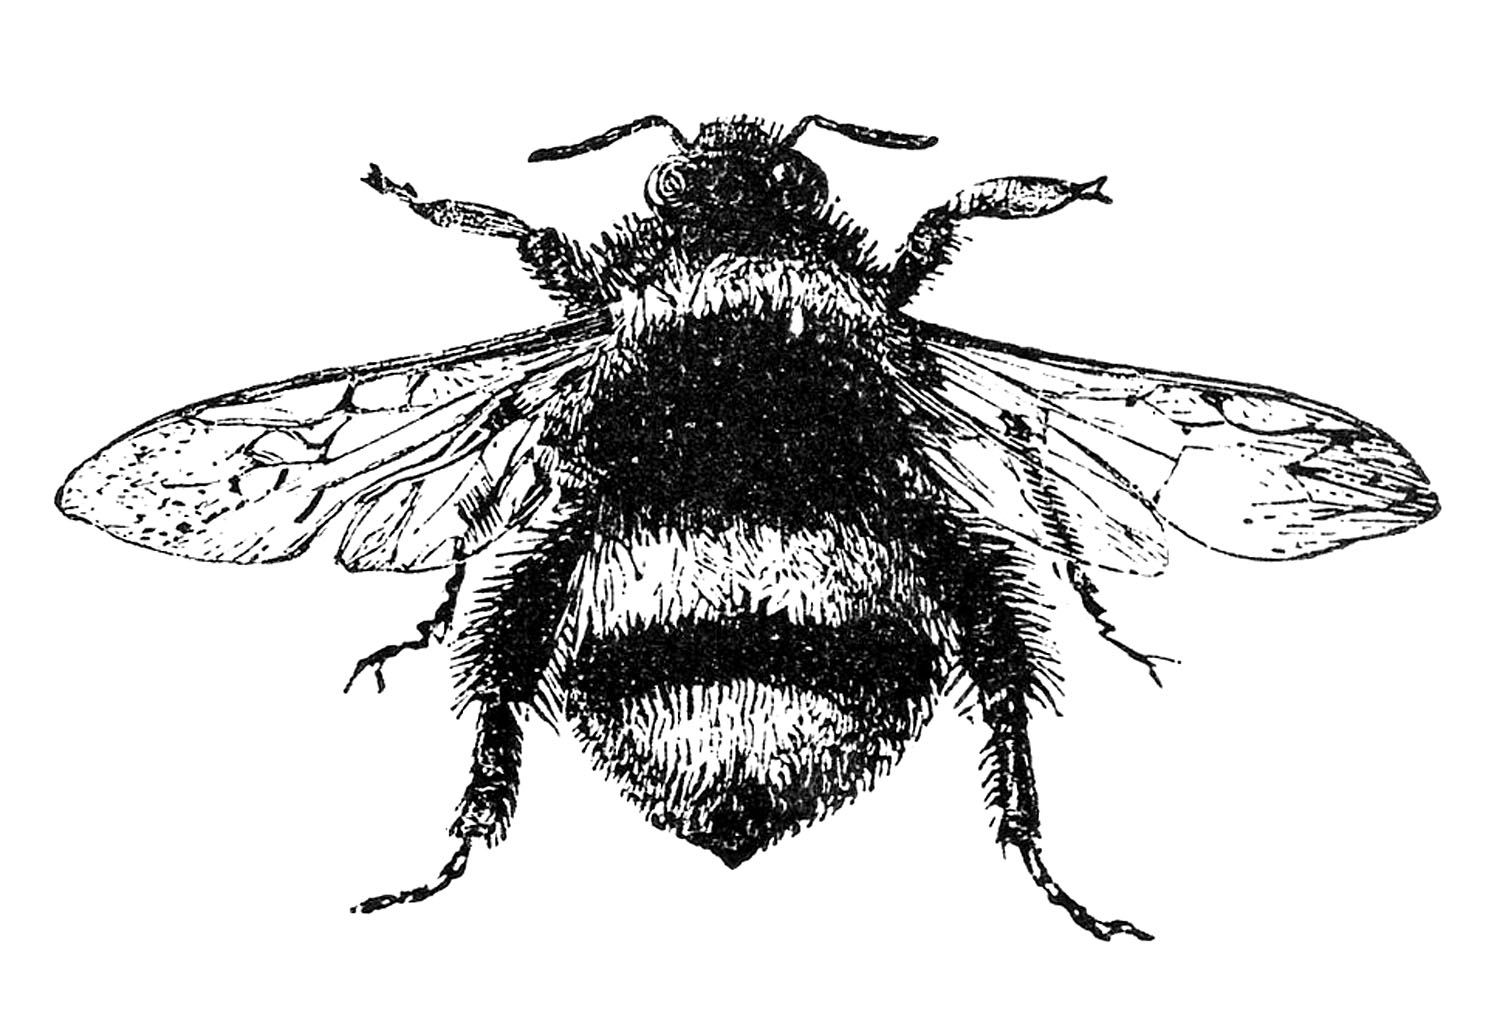
\includegraphics[scale=0.75]{img/bumblebee.jpg}
		\end{figure}
		\vspace{0.5cm}
		\Huge
		\textbf{\textsc{Metody Probabilistyczne Informatyki}}

		\vspace{0.5cm}
		\Large
		\textsc{Wybrane Dowody}

		\normalsize


		\line(1,0){330}

		\vspace{1cm}
		\textit{,,Tak teraz na to patrzę i myślę, czy ta nierówność nie powinna być w drugą stronę...''}
		\vspace{1cm}

		\textit{\textsc{Popełnione przez}}\\
		\vspace{5mm}

		\textbf{\textsc{
				Załatany Ponton \\
				V\\
				Nahtamatu\\
			}}

		\vfill

		Kraków \\
		Anno Domini 2025

	\end{center}

\end{titlepage}


\tableofcontents
\section*{Licencja}
\begin{figure}[h]
	\begin{minipage}[c]{0.25\textwidth}
		
\includegraphics[width=0.7\textwidth]{img/licencja.png}
	\end{minipage}\hfill
	\begin{minipage}[c]{0.75\textwidth}
		\caption*{
			Ten utwór jest dostępny na
			\href{https://creativecommons.org/licenses/by-sa/4.0/}{licencji Creative Commons Uznanie autorstwa
				na tych samych warunkach 4.0 Międzynarodowe.}
		}
	\end{minipage}
\end{figure}

% Remove the "Rozdział x" chapter headings, as we already number our chapters
\titleformat{\chapter}[display]{\normalfont\Huge\bfseries}{}{0pt}{\Huge}
\titlespacing*{\chapter}{0pt}{0pt}{20pt}

% Actual content
\mainmatter

\chapter{Wykład 1 (2025-10-03)}
 % Żeby nie było syfu to kolejne sekcje dodajemy do chapters/
% A potem includujemy za pomocą \input{chapters/...}

% Używamy \( \) i \[ \] zamiast dolarów -- tak jak się robi w LaTeXu


\documentclass[12pt, a4paper, polish, openany]{book}

% Please, let's familiarize ourselves with notatki.sty and tcs.sty so that we don't reinvent the wheel
\usepackage{notatki}
\fancyhead[L]{\textbf{\textit{MPI}}}

\begin{document}
% Front page and table of contents
\frontmatter

\input{titlepage}

\tableofcontents
\input{license}

% Remove the "Rozdział x" chapter headings, as we already number our chapters
\titleformat{\chapter}[display]{\normalfont\Huge\bfseries}{}{0pt}{\Huge}
\titlespacing*{\chapter}{0pt}{0pt}{20pt}

% Actual content
\mainmatter

\chapter{Wykład 1 (2025-10-03)}
\input{chapters/2025-10-03-lecture/main}

\chapter{Nagranie 1 (2025-10-04)}
\input{chapters/2025-10-04-recording/main}

\chapter{Wykład 2 (2025-10-10)}
\input{chapters/2025-10-10-lecture/main}

\chapter{Nagranie 2 (2025-10-10)}
\input{chapters/2025-10-10-recording/main}

\chapter{Wykład 3 (2025-10-17)}
\input{chapters/2025-10-17-lecture/main}

\end{document}


\chapter{Nagranie 1 (2025-10-04)}
 % Żeby nie było syfu to kolejne sekcje dodajemy do chapters/
% A potem includujemy za pomocą \input{chapters/...}

% Używamy \( \) i \[ \] zamiast dolarów -- tak jak się robi w LaTeXu


\documentclass[12pt, a4paper, polish, openany]{book}

% Please, let's familiarize ourselves with notatki.sty and tcs.sty so that we don't reinvent the wheel
\usepackage{notatki}
\fancyhead[L]{\textbf{\textit{MPI}}}

\begin{document}
% Front page and table of contents
\frontmatter

\input{titlepage}

\tableofcontents
\input{license}

% Remove the "Rozdział x" chapter headings, as we already number our chapters
\titleformat{\chapter}[display]{\normalfont\Huge\bfseries}{}{0pt}{\Huge}
\titlespacing*{\chapter}{0pt}{0pt}{20pt}

% Actual content
\mainmatter

\chapter{Wykład 1 (2025-10-03)}
\input{chapters/2025-10-03-lecture/main}

\chapter{Nagranie 1 (2025-10-04)}
\input{chapters/2025-10-04-recording/main}

\chapter{Wykład 2 (2025-10-10)}
\input{chapters/2025-10-10-lecture/main}

\chapter{Nagranie 2 (2025-10-10)}
\input{chapters/2025-10-10-recording/main}

\chapter{Wykład 3 (2025-10-17)}
\input{chapters/2025-10-17-lecture/main}

\end{document}


\chapter{Wykład 2 (2025-10-10)}
 % Żeby nie było syfu to kolejne sekcje dodajemy do chapters/
% A potem includujemy za pomocą \input{chapters/...}

% Używamy \( \) i \[ \] zamiast dolarów -- tak jak się robi w LaTeXu


\documentclass[12pt, a4paper, polish, openany]{book}

% Please, let's familiarize ourselves with notatki.sty and tcs.sty so that we don't reinvent the wheel
\usepackage{notatki}
\fancyhead[L]{\textbf{\textit{MPI}}}

\begin{document}
% Front page and table of contents
\frontmatter

\input{titlepage}

\tableofcontents
\input{license}

% Remove the "Rozdział x" chapter headings, as we already number our chapters
\titleformat{\chapter}[display]{\normalfont\Huge\bfseries}{}{0pt}{\Huge}
\titlespacing*{\chapter}{0pt}{0pt}{20pt}

% Actual content
\mainmatter

\chapter{Wykład 1 (2025-10-03)}
\input{chapters/2025-10-03-lecture/main}

\chapter{Nagranie 1 (2025-10-04)}
\input{chapters/2025-10-04-recording/main}

\chapter{Wykład 2 (2025-10-10)}
\input{chapters/2025-10-10-lecture/main}

\chapter{Nagranie 2 (2025-10-10)}
\input{chapters/2025-10-10-recording/main}

\chapter{Wykład 3 (2025-10-17)}
\input{chapters/2025-10-17-lecture/main}

\end{document}


\chapter{Nagranie 2 (2025-10-10)}
 % Żeby nie było syfu to kolejne sekcje dodajemy do chapters/
% A potem includujemy za pomocą \input{chapters/...}

% Używamy \( \) i \[ \] zamiast dolarów -- tak jak się robi w LaTeXu


\documentclass[12pt, a4paper, polish, openany]{book}

% Please, let's familiarize ourselves with notatki.sty and tcs.sty so that we don't reinvent the wheel
\usepackage{notatki}
\fancyhead[L]{\textbf{\textit{MPI}}}

\begin{document}
% Front page and table of contents
\frontmatter

\input{titlepage}

\tableofcontents
\input{license}

% Remove the "Rozdział x" chapter headings, as we already number our chapters
\titleformat{\chapter}[display]{\normalfont\Huge\bfseries}{}{0pt}{\Huge}
\titlespacing*{\chapter}{0pt}{0pt}{20pt}

% Actual content
\mainmatter

\chapter{Wykład 1 (2025-10-03)}
\input{chapters/2025-10-03-lecture/main}

\chapter{Nagranie 1 (2025-10-04)}
\input{chapters/2025-10-04-recording/main}

\chapter{Wykład 2 (2025-10-10)}
\input{chapters/2025-10-10-lecture/main}

\chapter{Nagranie 2 (2025-10-10)}
\input{chapters/2025-10-10-recording/main}

\chapter{Wykład 3 (2025-10-17)}
\input{chapters/2025-10-17-lecture/main}

\end{document}


\chapter{Wykład 3 (2025-10-17)}
 % Żeby nie było syfu to kolejne sekcje dodajemy do chapters/
% A potem includujemy za pomocą \input{chapters/...}

% Używamy \( \) i \[ \] zamiast dolarów -- tak jak się robi w LaTeXu


\documentclass[12pt, a4paper, polish, openany]{book}

% Please, let's familiarize ourselves with notatki.sty and tcs.sty so that we don't reinvent the wheel
\usepackage{notatki}
\fancyhead[L]{\textbf{\textit{MPI}}}

\begin{document}
% Front page and table of contents
\frontmatter

\input{titlepage}

\tableofcontents
\input{license}

% Remove the "Rozdział x" chapter headings, as we already number our chapters
\titleformat{\chapter}[display]{\normalfont\Huge\bfseries}{}{0pt}{\Huge}
\titlespacing*{\chapter}{0pt}{0pt}{20pt}

% Actual content
\mainmatter

\chapter{Wykład 1 (2025-10-03)}
\input{chapters/2025-10-03-lecture/main}

\chapter{Nagranie 1 (2025-10-04)}
\input{chapters/2025-10-04-recording/main}

\chapter{Wykład 2 (2025-10-10)}
\input{chapters/2025-10-10-lecture/main}

\chapter{Nagranie 2 (2025-10-10)}
\input{chapters/2025-10-10-recording/main}

\chapter{Wykład 3 (2025-10-17)}
\input{chapters/2025-10-17-lecture/main}

\end{document}


\end{document}


\chapter{Nagranie 2 (2025-10-10)}
 % Żeby nie było syfu to kolejne sekcje dodajemy do chapters/
% A potem includujemy za pomocą \input{chapters/...}

% Używamy \( \) i \[ \] zamiast dolarów -- tak jak się robi w LaTeXu


\documentclass[12pt, a4paper, polish, openany]{book}

% Please, let's familiarize ourselves with notatki.sty and tcs.sty so that we don't reinvent the wheel
\usepackage{notatki}
\fancyhead[L]{\textbf{\textit{MPI}}}

\begin{document}
% Front page and table of contents
\frontmatter

\begin{titlepage}

	\begin{center}
		\begin{figure}[h]
			\centering
			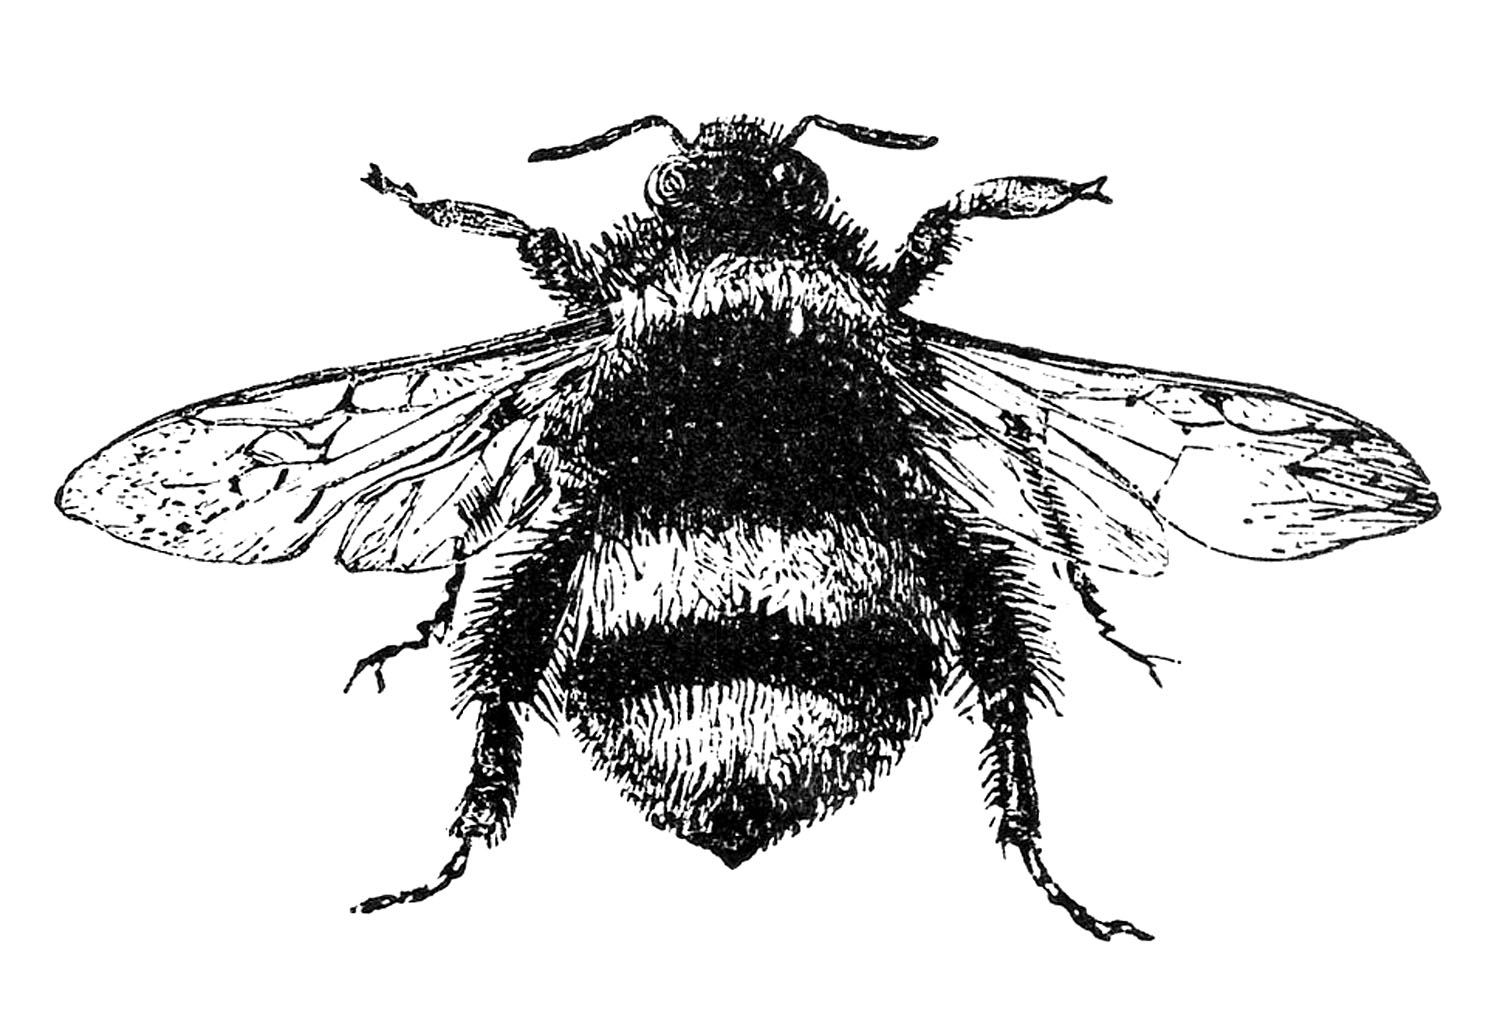
\includegraphics[scale=0.75]{img/bumblebee.jpg}
		\end{figure}
		\vspace{0.5cm}
		\Huge
		\textbf{\textsc{Metody Probabilistyczne Informatyki}}

		\vspace{0.5cm}
		\Large
		\textsc{Wybrane Dowody}

		\normalsize


		\line(1,0){330}

		\vspace{1cm}
		\textit{,,Tak teraz na to patrzę i myślę, czy ta nierówność nie powinna być w drugą stronę...''}
		\vspace{1cm}

		\textit{\textsc{Popełnione przez}}\\
		\vspace{5mm}

		\textbf{\textsc{
				Załatany Ponton \\
				V\\
				Nahtamatu\\
			}}

		\vfill

		Kraków \\
		Anno Domini 2025

	\end{center}

\end{titlepage}


\tableofcontents
\section*{Licencja}
\begin{figure}[h]
	\begin{minipage}[c]{0.25\textwidth}
		
\includegraphics[width=0.7\textwidth]{img/licencja.png}
	\end{minipage}\hfill
	\begin{minipage}[c]{0.75\textwidth}
		\caption*{
			Ten utwór jest dostępny na
			\href{https://creativecommons.org/licenses/by-sa/4.0/}{licencji Creative Commons Uznanie autorstwa
				na tych samych warunkach 4.0 Międzynarodowe.}
		}
	\end{minipage}
\end{figure}

% Remove the "Rozdział x" chapter headings, as we already number our chapters
\titleformat{\chapter}[display]{\normalfont\Huge\bfseries}{}{0pt}{\Huge}
\titlespacing*{\chapter}{0pt}{0pt}{20pt}

% Actual content
\mainmatter

\chapter{Wykład 1 (2025-10-03)}
 % Żeby nie było syfu to kolejne sekcje dodajemy do chapters/
% A potem includujemy za pomocą \input{chapters/...}

% Używamy \( \) i \[ \] zamiast dolarów -- tak jak się robi w LaTeXu


\documentclass[12pt, a4paper, polish, openany]{book}

% Please, let's familiarize ourselves with notatki.sty and tcs.sty so that we don't reinvent the wheel
\usepackage{notatki}
\fancyhead[L]{\textbf{\textit{MPI}}}

\begin{document}
% Front page and table of contents
\frontmatter

\input{titlepage}

\tableofcontents
\input{license}

% Remove the "Rozdział x" chapter headings, as we already number our chapters
\titleformat{\chapter}[display]{\normalfont\Huge\bfseries}{}{0pt}{\Huge}
\titlespacing*{\chapter}{0pt}{0pt}{20pt}

% Actual content
\mainmatter

\chapter{Wykład 1 (2025-10-03)}
\input{chapters/2025-10-03-lecture/main}

\chapter{Nagranie 1 (2025-10-04)}
\input{chapters/2025-10-04-recording/main}

\chapter{Wykład 2 (2025-10-10)}
\input{chapters/2025-10-10-lecture/main}

\chapter{Nagranie 2 (2025-10-10)}
\input{chapters/2025-10-10-recording/main}

\chapter{Wykład 3 (2025-10-17)}
\input{chapters/2025-10-17-lecture/main}

\end{document}


\chapter{Nagranie 1 (2025-10-04)}
 % Żeby nie było syfu to kolejne sekcje dodajemy do chapters/
% A potem includujemy za pomocą \input{chapters/...}

% Używamy \( \) i \[ \] zamiast dolarów -- tak jak się robi w LaTeXu


\documentclass[12pt, a4paper, polish, openany]{book}

% Please, let's familiarize ourselves with notatki.sty and tcs.sty so that we don't reinvent the wheel
\usepackage{notatki}
\fancyhead[L]{\textbf{\textit{MPI}}}

\begin{document}
% Front page and table of contents
\frontmatter

\input{titlepage}

\tableofcontents
\input{license}

% Remove the "Rozdział x" chapter headings, as we already number our chapters
\titleformat{\chapter}[display]{\normalfont\Huge\bfseries}{}{0pt}{\Huge}
\titlespacing*{\chapter}{0pt}{0pt}{20pt}

% Actual content
\mainmatter

\chapter{Wykład 1 (2025-10-03)}
\input{chapters/2025-10-03-lecture/main}

\chapter{Nagranie 1 (2025-10-04)}
\input{chapters/2025-10-04-recording/main}

\chapter{Wykład 2 (2025-10-10)}
\input{chapters/2025-10-10-lecture/main}

\chapter{Nagranie 2 (2025-10-10)}
\input{chapters/2025-10-10-recording/main}

\chapter{Wykład 3 (2025-10-17)}
\input{chapters/2025-10-17-lecture/main}

\end{document}


\chapter{Wykład 2 (2025-10-10)}
 % Żeby nie było syfu to kolejne sekcje dodajemy do chapters/
% A potem includujemy za pomocą \input{chapters/...}

% Używamy \( \) i \[ \] zamiast dolarów -- tak jak się robi w LaTeXu


\documentclass[12pt, a4paper, polish, openany]{book}

% Please, let's familiarize ourselves with notatki.sty and tcs.sty so that we don't reinvent the wheel
\usepackage{notatki}
\fancyhead[L]{\textbf{\textit{MPI}}}

\begin{document}
% Front page and table of contents
\frontmatter

\input{titlepage}

\tableofcontents
\input{license}

% Remove the "Rozdział x" chapter headings, as we already number our chapters
\titleformat{\chapter}[display]{\normalfont\Huge\bfseries}{}{0pt}{\Huge}
\titlespacing*{\chapter}{0pt}{0pt}{20pt}

% Actual content
\mainmatter

\chapter{Wykład 1 (2025-10-03)}
\input{chapters/2025-10-03-lecture/main}

\chapter{Nagranie 1 (2025-10-04)}
\input{chapters/2025-10-04-recording/main}

\chapter{Wykład 2 (2025-10-10)}
\input{chapters/2025-10-10-lecture/main}

\chapter{Nagranie 2 (2025-10-10)}
\input{chapters/2025-10-10-recording/main}

\chapter{Wykład 3 (2025-10-17)}
\input{chapters/2025-10-17-lecture/main}

\end{document}


\chapter{Nagranie 2 (2025-10-10)}
 % Żeby nie było syfu to kolejne sekcje dodajemy do chapters/
% A potem includujemy za pomocą \input{chapters/...}

% Używamy \( \) i \[ \] zamiast dolarów -- tak jak się robi w LaTeXu


\documentclass[12pt, a4paper, polish, openany]{book}

% Please, let's familiarize ourselves with notatki.sty and tcs.sty so that we don't reinvent the wheel
\usepackage{notatki}
\fancyhead[L]{\textbf{\textit{MPI}}}

\begin{document}
% Front page and table of contents
\frontmatter

\input{titlepage}

\tableofcontents
\input{license}

% Remove the "Rozdział x" chapter headings, as we already number our chapters
\titleformat{\chapter}[display]{\normalfont\Huge\bfseries}{}{0pt}{\Huge}
\titlespacing*{\chapter}{0pt}{0pt}{20pt}

% Actual content
\mainmatter

\chapter{Wykład 1 (2025-10-03)}
\input{chapters/2025-10-03-lecture/main}

\chapter{Nagranie 1 (2025-10-04)}
\input{chapters/2025-10-04-recording/main}

\chapter{Wykład 2 (2025-10-10)}
\input{chapters/2025-10-10-lecture/main}

\chapter{Nagranie 2 (2025-10-10)}
\input{chapters/2025-10-10-recording/main}

\chapter{Wykład 3 (2025-10-17)}
\input{chapters/2025-10-17-lecture/main}

\end{document}


\chapter{Wykład 3 (2025-10-17)}
 % Żeby nie było syfu to kolejne sekcje dodajemy do chapters/
% A potem includujemy za pomocą \input{chapters/...}

% Używamy \( \) i \[ \] zamiast dolarów -- tak jak się robi w LaTeXu


\documentclass[12pt, a4paper, polish, openany]{book}

% Please, let's familiarize ourselves with notatki.sty and tcs.sty so that we don't reinvent the wheel
\usepackage{notatki}
\fancyhead[L]{\textbf{\textit{MPI}}}

\begin{document}
% Front page and table of contents
\frontmatter

\input{titlepage}

\tableofcontents
\input{license}

% Remove the "Rozdział x" chapter headings, as we already number our chapters
\titleformat{\chapter}[display]{\normalfont\Huge\bfseries}{}{0pt}{\Huge}
\titlespacing*{\chapter}{0pt}{0pt}{20pt}

% Actual content
\mainmatter

\chapter{Wykład 1 (2025-10-03)}
\input{chapters/2025-10-03-lecture/main}

\chapter{Nagranie 1 (2025-10-04)}
\input{chapters/2025-10-04-recording/main}

\chapter{Wykład 2 (2025-10-10)}
\input{chapters/2025-10-10-lecture/main}

\chapter{Nagranie 2 (2025-10-10)}
\input{chapters/2025-10-10-recording/main}

\chapter{Wykład 3 (2025-10-17)}
\input{chapters/2025-10-17-lecture/main}

\end{document}


\end{document}


\chapter{Wykład 3 (2025-10-17)}
 % Żeby nie było syfu to kolejne sekcje dodajemy do chapters/
% A potem includujemy za pomocą \input{chapters/...}

% Używamy \( \) i \[ \] zamiast dolarów -- tak jak się robi w LaTeXu


\documentclass[12pt, a4paper, polish, openany]{book}

% Please, let's familiarize ourselves with notatki.sty and tcs.sty so that we don't reinvent the wheel
\usepackage{notatki}
\fancyhead[L]{\textbf{\textit{MPI}}}

\begin{document}
% Front page and table of contents
\frontmatter

\begin{titlepage}

	\begin{center}
		\begin{figure}[h]
			\centering
			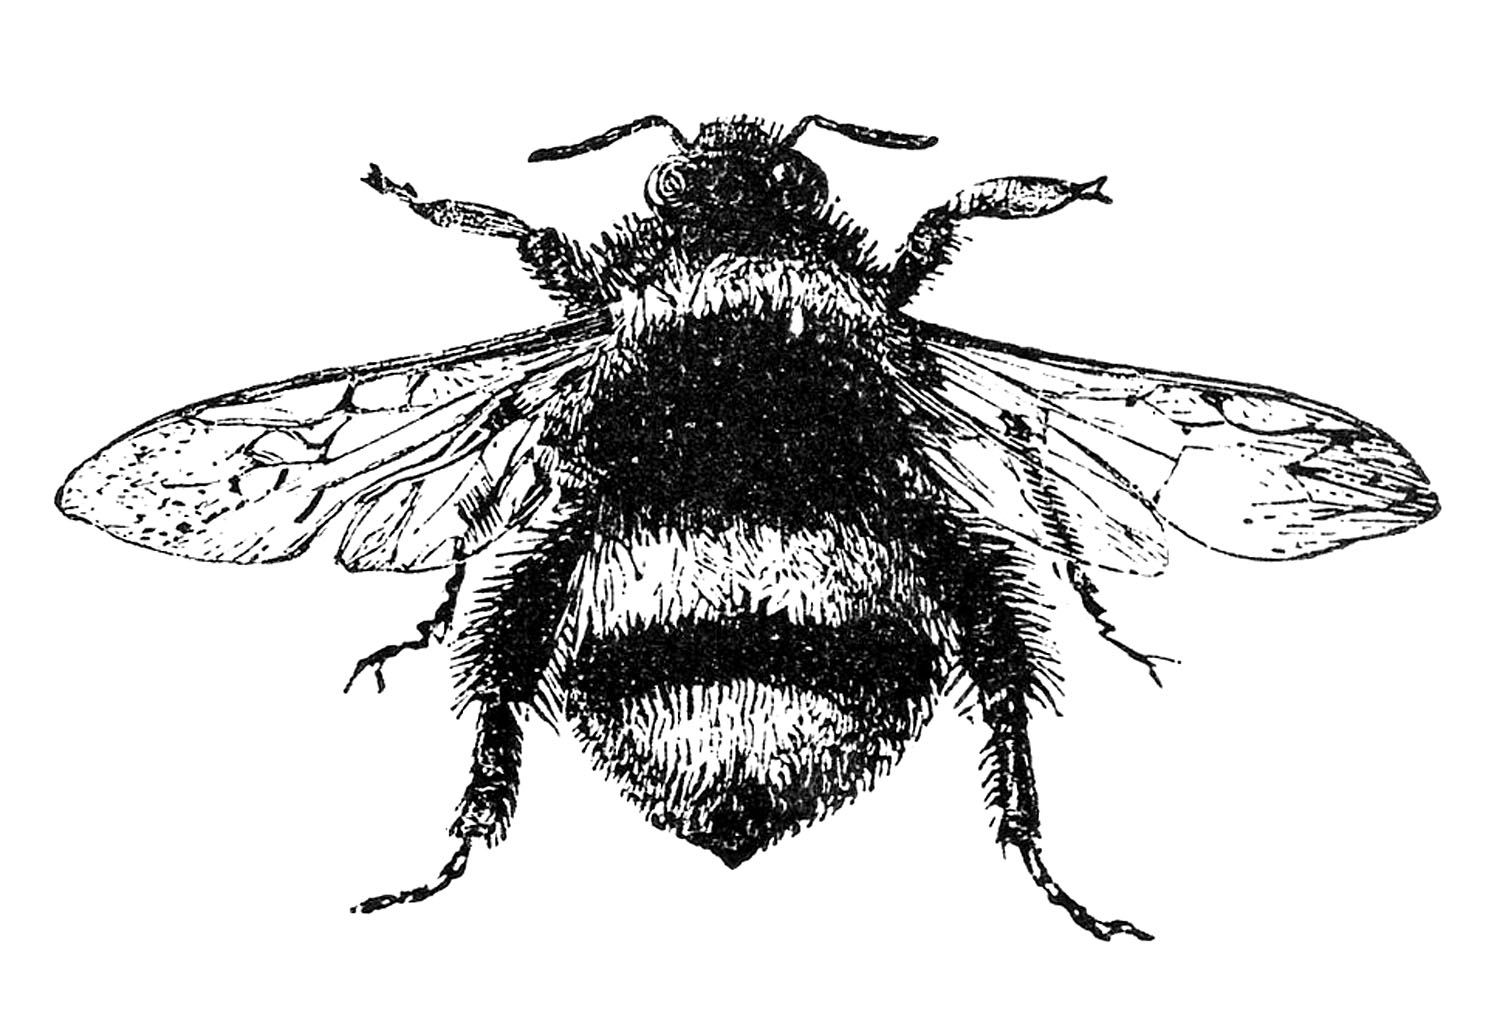
\includegraphics[scale=0.75]{img/bumblebee.jpg}
		\end{figure}
		\vspace{0.5cm}
		\Huge
		\textbf{\textsc{Metody Probabilistyczne Informatyki}}

		\vspace{0.5cm}
		\Large
		\textsc{Wybrane Dowody}

		\normalsize


		\line(1,0){330}

		\vspace{1cm}
		\textit{,,Tak teraz na to patrzę i myślę, czy ta nierówność nie powinna być w drugą stronę...''}
		\vspace{1cm}

		\textit{\textsc{Popełnione przez}}\\
		\vspace{5mm}

		\textbf{\textsc{
				Załatany Ponton \\
				V\\
				Nahtamatu\\
			}}

		\vfill

		Kraków \\
		Anno Domini 2025

	\end{center}

\end{titlepage}


\tableofcontents
\section*{Licencja}
\begin{figure}[h]
	\begin{minipage}[c]{0.25\textwidth}
		
\includegraphics[width=0.7\textwidth]{img/licencja.png}
	\end{minipage}\hfill
	\begin{minipage}[c]{0.75\textwidth}
		\caption*{
			Ten utwór jest dostępny na
			\href{https://creativecommons.org/licenses/by-sa/4.0/}{licencji Creative Commons Uznanie autorstwa
				na tych samych warunkach 4.0 Międzynarodowe.}
		}
	\end{minipage}
\end{figure}

% Remove the "Rozdział x" chapter headings, as we already number our chapters
\titleformat{\chapter}[display]{\normalfont\Huge\bfseries}{}{0pt}{\Huge}
\titlespacing*{\chapter}{0pt}{0pt}{20pt}

% Actual content
\mainmatter

\chapter{Wykład 1 (2025-10-03)}
 % Żeby nie było syfu to kolejne sekcje dodajemy do chapters/
% A potem includujemy za pomocą \input{chapters/...}

% Używamy \( \) i \[ \] zamiast dolarów -- tak jak się robi w LaTeXu


\documentclass[12pt, a4paper, polish, openany]{book}

% Please, let's familiarize ourselves with notatki.sty and tcs.sty so that we don't reinvent the wheel
\usepackage{notatki}
\fancyhead[L]{\textbf{\textit{MPI}}}

\begin{document}
% Front page and table of contents
\frontmatter

\input{titlepage}

\tableofcontents
\input{license}

% Remove the "Rozdział x" chapter headings, as we already number our chapters
\titleformat{\chapter}[display]{\normalfont\Huge\bfseries}{}{0pt}{\Huge}
\titlespacing*{\chapter}{0pt}{0pt}{20pt}

% Actual content
\mainmatter

\chapter{Wykład 1 (2025-10-03)}
\input{chapters/2025-10-03-lecture/main}

\chapter{Nagranie 1 (2025-10-04)}
\input{chapters/2025-10-04-recording/main}

\chapter{Wykład 2 (2025-10-10)}
\input{chapters/2025-10-10-lecture/main}

\chapter{Nagranie 2 (2025-10-10)}
\input{chapters/2025-10-10-recording/main}

\chapter{Wykład 3 (2025-10-17)}
\input{chapters/2025-10-17-lecture/main}

\end{document}


\chapter{Nagranie 1 (2025-10-04)}
 % Żeby nie było syfu to kolejne sekcje dodajemy do chapters/
% A potem includujemy za pomocą \input{chapters/...}

% Używamy \( \) i \[ \] zamiast dolarów -- tak jak się robi w LaTeXu


\documentclass[12pt, a4paper, polish, openany]{book}

% Please, let's familiarize ourselves with notatki.sty and tcs.sty so that we don't reinvent the wheel
\usepackage{notatki}
\fancyhead[L]{\textbf{\textit{MPI}}}

\begin{document}
% Front page and table of contents
\frontmatter

\input{titlepage}

\tableofcontents
\input{license}

% Remove the "Rozdział x" chapter headings, as we already number our chapters
\titleformat{\chapter}[display]{\normalfont\Huge\bfseries}{}{0pt}{\Huge}
\titlespacing*{\chapter}{0pt}{0pt}{20pt}

% Actual content
\mainmatter

\chapter{Wykład 1 (2025-10-03)}
\input{chapters/2025-10-03-lecture/main}

\chapter{Nagranie 1 (2025-10-04)}
\input{chapters/2025-10-04-recording/main}

\chapter{Wykład 2 (2025-10-10)}
\input{chapters/2025-10-10-lecture/main}

\chapter{Nagranie 2 (2025-10-10)}
\input{chapters/2025-10-10-recording/main}

\chapter{Wykład 3 (2025-10-17)}
\input{chapters/2025-10-17-lecture/main}

\end{document}


\chapter{Wykład 2 (2025-10-10)}
 % Żeby nie było syfu to kolejne sekcje dodajemy do chapters/
% A potem includujemy za pomocą \input{chapters/...}

% Używamy \( \) i \[ \] zamiast dolarów -- tak jak się robi w LaTeXu


\documentclass[12pt, a4paper, polish, openany]{book}

% Please, let's familiarize ourselves with notatki.sty and tcs.sty so that we don't reinvent the wheel
\usepackage{notatki}
\fancyhead[L]{\textbf{\textit{MPI}}}

\begin{document}
% Front page and table of contents
\frontmatter

\input{titlepage}

\tableofcontents
\input{license}

% Remove the "Rozdział x" chapter headings, as we already number our chapters
\titleformat{\chapter}[display]{\normalfont\Huge\bfseries}{}{0pt}{\Huge}
\titlespacing*{\chapter}{0pt}{0pt}{20pt}

% Actual content
\mainmatter

\chapter{Wykład 1 (2025-10-03)}
\input{chapters/2025-10-03-lecture/main}

\chapter{Nagranie 1 (2025-10-04)}
\input{chapters/2025-10-04-recording/main}

\chapter{Wykład 2 (2025-10-10)}
\input{chapters/2025-10-10-lecture/main}

\chapter{Nagranie 2 (2025-10-10)}
\input{chapters/2025-10-10-recording/main}

\chapter{Wykład 3 (2025-10-17)}
\input{chapters/2025-10-17-lecture/main}

\end{document}


\chapter{Nagranie 2 (2025-10-10)}
 % Żeby nie było syfu to kolejne sekcje dodajemy do chapters/
% A potem includujemy za pomocą \input{chapters/...}

% Używamy \( \) i \[ \] zamiast dolarów -- tak jak się robi w LaTeXu


\documentclass[12pt, a4paper, polish, openany]{book}

% Please, let's familiarize ourselves with notatki.sty and tcs.sty so that we don't reinvent the wheel
\usepackage{notatki}
\fancyhead[L]{\textbf{\textit{MPI}}}

\begin{document}
% Front page and table of contents
\frontmatter

\input{titlepage}

\tableofcontents
\input{license}

% Remove the "Rozdział x" chapter headings, as we already number our chapters
\titleformat{\chapter}[display]{\normalfont\Huge\bfseries}{}{0pt}{\Huge}
\titlespacing*{\chapter}{0pt}{0pt}{20pt}

% Actual content
\mainmatter

\chapter{Wykład 1 (2025-10-03)}
\input{chapters/2025-10-03-lecture/main}

\chapter{Nagranie 1 (2025-10-04)}
\input{chapters/2025-10-04-recording/main}

\chapter{Wykład 2 (2025-10-10)}
\input{chapters/2025-10-10-lecture/main}

\chapter{Nagranie 2 (2025-10-10)}
\input{chapters/2025-10-10-recording/main}

\chapter{Wykład 3 (2025-10-17)}
\input{chapters/2025-10-17-lecture/main}

\end{document}


\chapter{Wykład 3 (2025-10-17)}
 % Żeby nie było syfu to kolejne sekcje dodajemy do chapters/
% A potem includujemy za pomocą \input{chapters/...}

% Używamy \( \) i \[ \] zamiast dolarów -- tak jak się robi w LaTeXu


\documentclass[12pt, a4paper, polish, openany]{book}

% Please, let's familiarize ourselves with notatki.sty and tcs.sty so that we don't reinvent the wheel
\usepackage{notatki}
\fancyhead[L]{\textbf{\textit{MPI}}}

\begin{document}
% Front page and table of contents
\frontmatter

\input{titlepage}

\tableofcontents
\input{license}

% Remove the "Rozdział x" chapter headings, as we already number our chapters
\titleformat{\chapter}[display]{\normalfont\Huge\bfseries}{}{0pt}{\Huge}
\titlespacing*{\chapter}{0pt}{0pt}{20pt}

% Actual content
\mainmatter

\chapter{Wykład 1 (2025-10-03)}
\input{chapters/2025-10-03-lecture/main}

\chapter{Nagranie 1 (2025-10-04)}
\input{chapters/2025-10-04-recording/main}

\chapter{Wykład 2 (2025-10-10)}
\input{chapters/2025-10-10-lecture/main}

\chapter{Nagranie 2 (2025-10-10)}
\input{chapters/2025-10-10-recording/main}

\chapter{Wykład 3 (2025-10-17)}
\input{chapters/2025-10-17-lecture/main}

\end{document}


\end{document}


\end{document}


\realsection{Twierdzenie Ramseya. Przykłady zastosowań}
 % Żeby nie było syfu to kolejne sekcje dodajemy do chapters/
% A potem includujemy za pomocą \input{chapters/...}

% Używamy \( \) i \[ \] zamiast dolarów -- tak jak się robi w LaTeXu


\documentclass[12pt, a4paper, polish, openany]{book}

% Please, let's familiarize ourselves with notatki.sty and tcs.sty so that we don't reinvent the wheel
\usepackage{notatki}
\fancyhead[L]{\textbf{\textit{MPI}}}

\begin{document}
% Front page and table of contents
\frontmatter

\begin{titlepage}

	\begin{center}
		\begin{figure}[h]
			\centering
			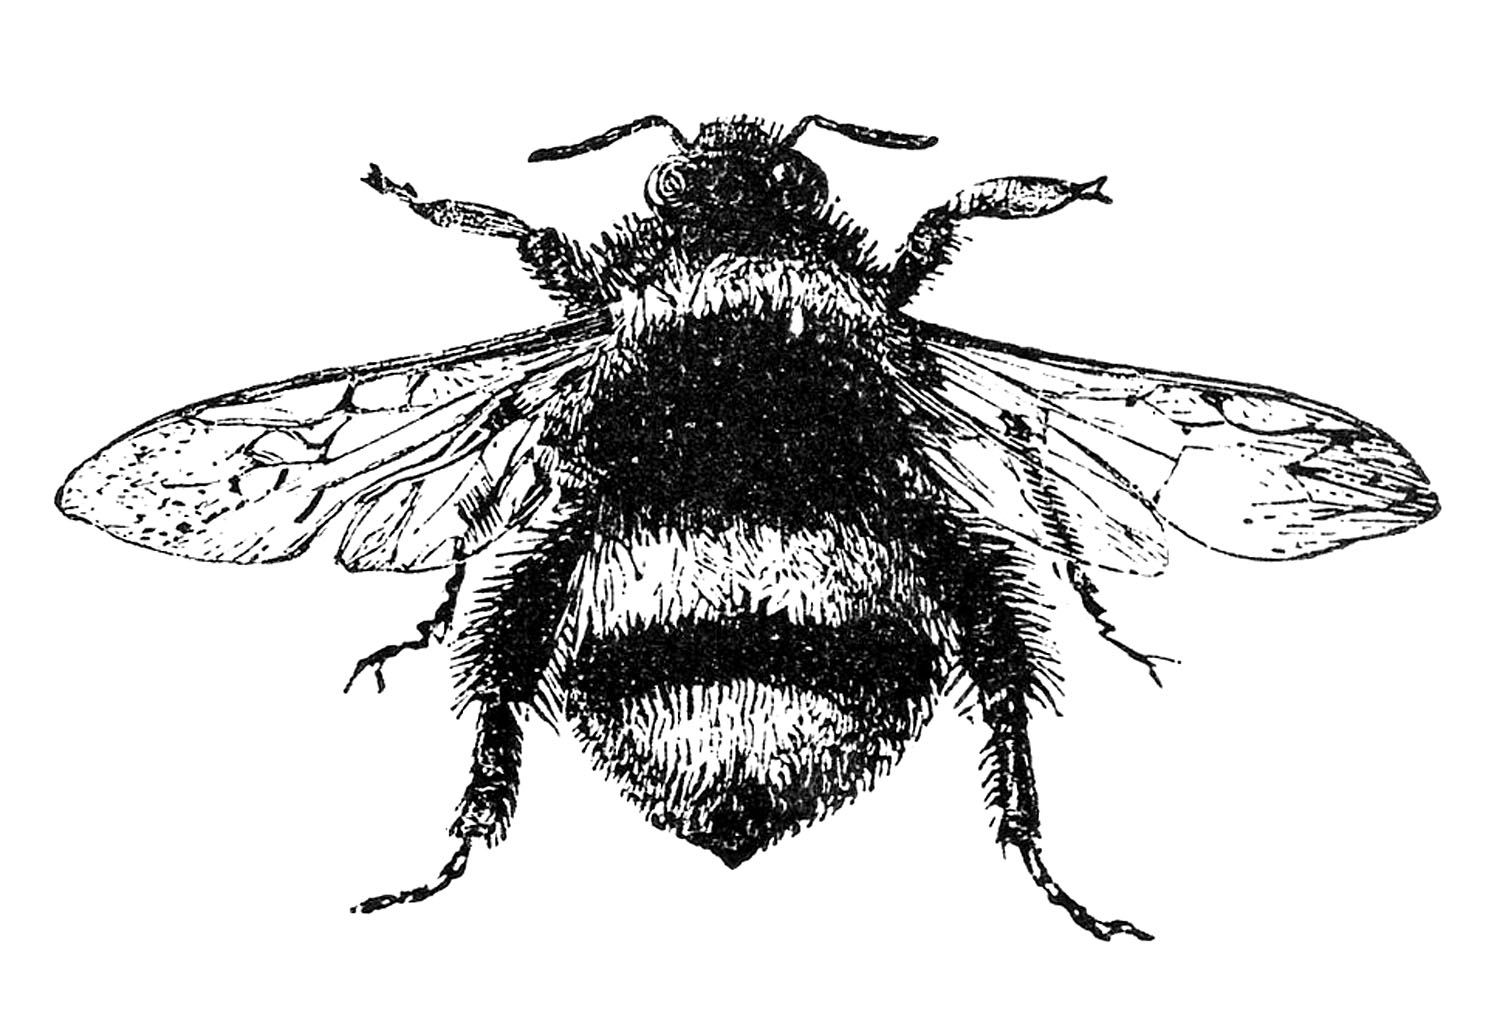
\includegraphics[scale=0.75]{img/bumblebee.jpg}
		\end{figure}
		\vspace{0.5cm}
		\Huge
		\textbf{\textsc{Metody Probabilistyczne Informatyki}}

		\vspace{0.5cm}
		\Large
		\textsc{Wybrane Dowody}

		\normalsize


		\line(1,0){330}

		\vspace{1cm}
		\textit{,,Tak teraz na to patrzę i myślę, czy ta nierówność nie powinna być w drugą stronę...''}
		\vspace{1cm}

		\textit{\textsc{Popełnione przez}}\\
		\vspace{5mm}

		\textbf{\textsc{
				Załatany Ponton \\
				V\\
				Nahtamatu\\
			}}

		\vfill

		Kraków \\
		Anno Domini 2025

	\end{center}

\end{titlepage}


\tableofcontents
\section*{Licencja}
\begin{figure}[h]
	\begin{minipage}[c]{0.25\textwidth}
		
\includegraphics[width=0.7\textwidth]{img/licencja.png}
	\end{minipage}\hfill
	\begin{minipage}[c]{0.75\textwidth}
		\caption*{
			Ten utwór jest dostępny na
			\href{https://creativecommons.org/licenses/by-sa/4.0/}{licencji Creative Commons Uznanie autorstwa
				na tych samych warunkach 4.0 Międzynarodowe.}
		}
	\end{minipage}
\end{figure}

% Remove the "Rozdział x" chapter headings, as we already number our chapters
\titleformat{\chapter}[display]{\normalfont\Huge\bfseries}{}{0pt}{\Huge}
\titlespacing*{\chapter}{0pt}{0pt}{20pt}

% Actual content
\mainmatter

\chapter{Wykład 1 (2025-10-03)}
 % Żeby nie było syfu to kolejne sekcje dodajemy do chapters/
% A potem includujemy za pomocą \input{chapters/...}

% Używamy \( \) i \[ \] zamiast dolarów -- tak jak się robi w LaTeXu


\documentclass[12pt, a4paper, polish, openany]{book}

% Please, let's familiarize ourselves with notatki.sty and tcs.sty so that we don't reinvent the wheel
\usepackage{notatki}
\fancyhead[L]{\textbf{\textit{MPI}}}

\begin{document}
% Front page and table of contents
\frontmatter

\begin{titlepage}

	\begin{center}
		\begin{figure}[h]
			\centering
			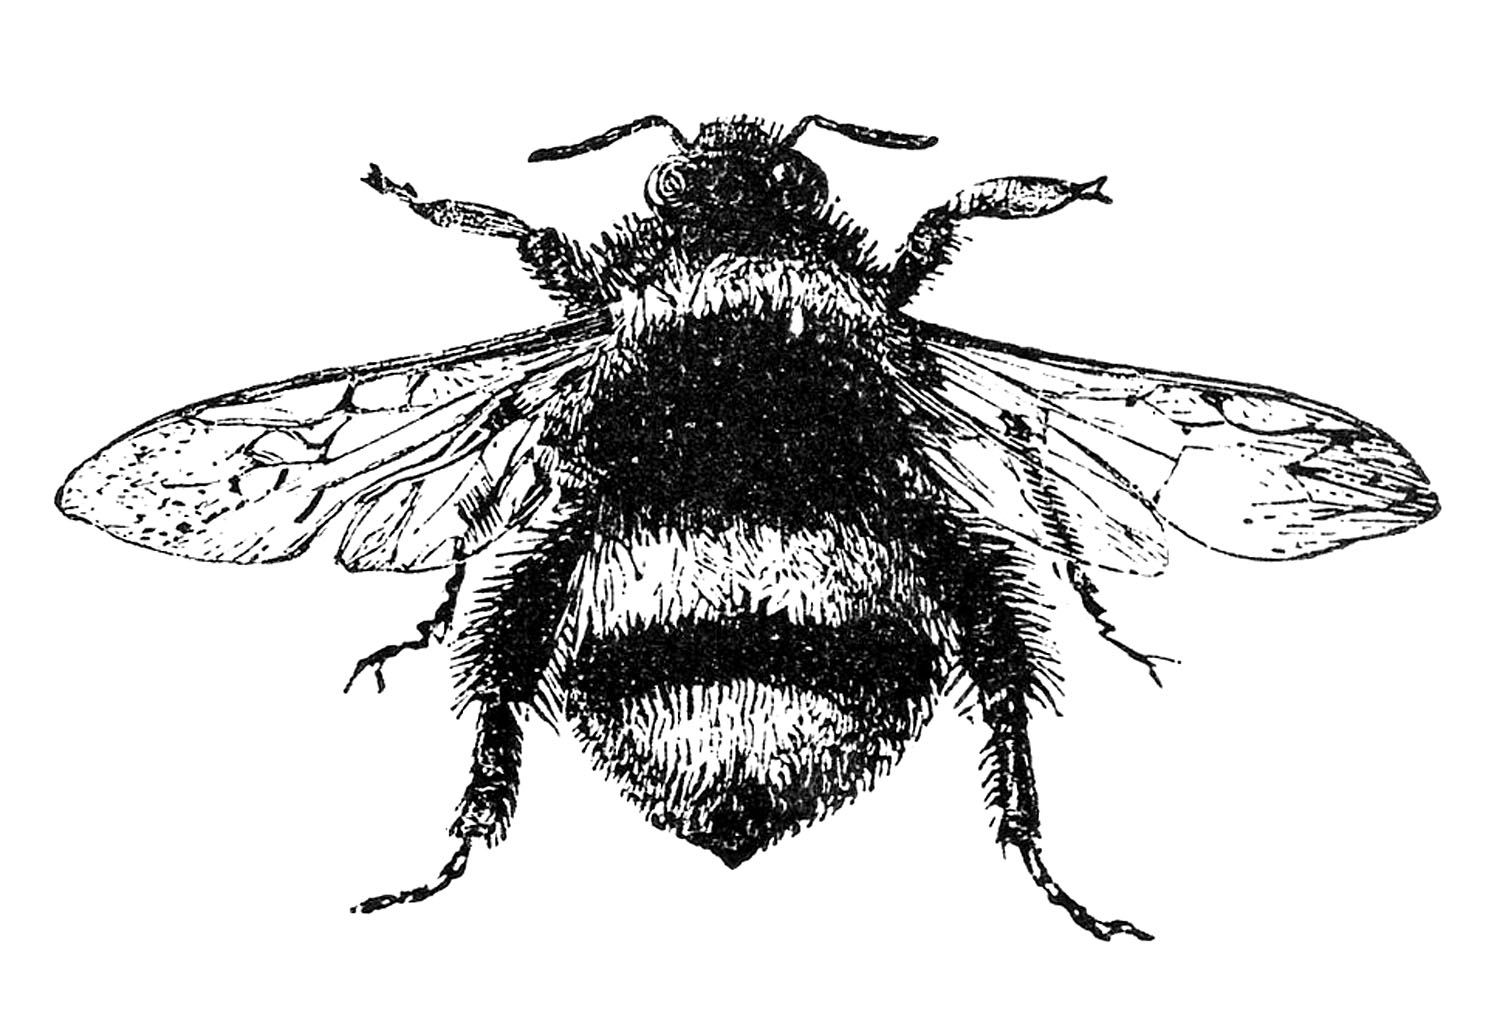
\includegraphics[scale=0.75]{img/bumblebee.jpg}
		\end{figure}
		\vspace{0.5cm}
		\Huge
		\textbf{\textsc{Metody Probabilistyczne Informatyki}}

		\vspace{0.5cm}
		\Large
		\textsc{Wybrane Dowody}

		\normalsize


		\line(1,0){330}

		\vspace{1cm}
		\textit{,,Tak teraz na to patrzę i myślę, czy ta nierówność nie powinna być w drugą stronę...''}
		\vspace{1cm}

		\textit{\textsc{Popełnione przez}}\\
		\vspace{5mm}

		\textbf{\textsc{
				Załatany Ponton \\
				V\\
				Nahtamatu\\
			}}

		\vfill

		Kraków \\
		Anno Domini 2025

	\end{center}

\end{titlepage}


\tableofcontents
\section*{Licencja}
\begin{figure}[h]
	\begin{minipage}[c]{0.25\textwidth}
		
\includegraphics[width=0.7\textwidth]{img/licencja.png}
	\end{minipage}\hfill
	\begin{minipage}[c]{0.75\textwidth}
		\caption*{
			Ten utwór jest dostępny na
			\href{https://creativecommons.org/licenses/by-sa/4.0/}{licencji Creative Commons Uznanie autorstwa
				na tych samych warunkach 4.0 Międzynarodowe.}
		}
	\end{minipage}
\end{figure}

% Remove the "Rozdział x" chapter headings, as we already number our chapters
\titleformat{\chapter}[display]{\normalfont\Huge\bfseries}{}{0pt}{\Huge}
\titlespacing*{\chapter}{0pt}{0pt}{20pt}

% Actual content
\mainmatter

\chapter{Wykład 1 (2025-10-03)}
 % Żeby nie było syfu to kolejne sekcje dodajemy do chapters/
% A potem includujemy za pomocą \input{chapters/...}

% Używamy \( \) i \[ \] zamiast dolarów -- tak jak się robi w LaTeXu


\documentclass[12pt, a4paper, polish, openany]{book}

% Please, let's familiarize ourselves with notatki.sty and tcs.sty so that we don't reinvent the wheel
\usepackage{notatki}
\fancyhead[L]{\textbf{\textit{MPI}}}

\begin{document}
% Front page and table of contents
\frontmatter

\input{titlepage}

\tableofcontents
\input{license}

% Remove the "Rozdział x" chapter headings, as we already number our chapters
\titleformat{\chapter}[display]{\normalfont\Huge\bfseries}{}{0pt}{\Huge}
\titlespacing*{\chapter}{0pt}{0pt}{20pt}

% Actual content
\mainmatter

\chapter{Wykład 1 (2025-10-03)}
\input{chapters/2025-10-03-lecture/main}

\chapter{Nagranie 1 (2025-10-04)}
\input{chapters/2025-10-04-recording/main}

\chapter{Wykład 2 (2025-10-10)}
\input{chapters/2025-10-10-lecture/main}

\chapter{Nagranie 2 (2025-10-10)}
\input{chapters/2025-10-10-recording/main}

\chapter{Wykład 3 (2025-10-17)}
\input{chapters/2025-10-17-lecture/main}

\end{document}


\chapter{Nagranie 1 (2025-10-04)}
 % Żeby nie było syfu to kolejne sekcje dodajemy do chapters/
% A potem includujemy za pomocą \input{chapters/...}

% Używamy \( \) i \[ \] zamiast dolarów -- tak jak się robi w LaTeXu


\documentclass[12pt, a4paper, polish, openany]{book}

% Please, let's familiarize ourselves with notatki.sty and tcs.sty so that we don't reinvent the wheel
\usepackage{notatki}
\fancyhead[L]{\textbf{\textit{MPI}}}

\begin{document}
% Front page and table of contents
\frontmatter

\input{titlepage}

\tableofcontents
\input{license}

% Remove the "Rozdział x" chapter headings, as we already number our chapters
\titleformat{\chapter}[display]{\normalfont\Huge\bfseries}{}{0pt}{\Huge}
\titlespacing*{\chapter}{0pt}{0pt}{20pt}

% Actual content
\mainmatter

\chapter{Wykład 1 (2025-10-03)}
\input{chapters/2025-10-03-lecture/main}

\chapter{Nagranie 1 (2025-10-04)}
\input{chapters/2025-10-04-recording/main}

\chapter{Wykład 2 (2025-10-10)}
\input{chapters/2025-10-10-lecture/main}

\chapter{Nagranie 2 (2025-10-10)}
\input{chapters/2025-10-10-recording/main}

\chapter{Wykład 3 (2025-10-17)}
\input{chapters/2025-10-17-lecture/main}

\end{document}


\chapter{Wykład 2 (2025-10-10)}
 % Żeby nie było syfu to kolejne sekcje dodajemy do chapters/
% A potem includujemy za pomocą \input{chapters/...}

% Używamy \( \) i \[ \] zamiast dolarów -- tak jak się robi w LaTeXu


\documentclass[12pt, a4paper, polish, openany]{book}

% Please, let's familiarize ourselves with notatki.sty and tcs.sty so that we don't reinvent the wheel
\usepackage{notatki}
\fancyhead[L]{\textbf{\textit{MPI}}}

\begin{document}
% Front page and table of contents
\frontmatter

\input{titlepage}

\tableofcontents
\input{license}

% Remove the "Rozdział x" chapter headings, as we already number our chapters
\titleformat{\chapter}[display]{\normalfont\Huge\bfseries}{}{0pt}{\Huge}
\titlespacing*{\chapter}{0pt}{0pt}{20pt}

% Actual content
\mainmatter

\chapter{Wykład 1 (2025-10-03)}
\input{chapters/2025-10-03-lecture/main}

\chapter{Nagranie 1 (2025-10-04)}
\input{chapters/2025-10-04-recording/main}

\chapter{Wykład 2 (2025-10-10)}
\input{chapters/2025-10-10-lecture/main}

\chapter{Nagranie 2 (2025-10-10)}
\input{chapters/2025-10-10-recording/main}

\chapter{Wykład 3 (2025-10-17)}
\input{chapters/2025-10-17-lecture/main}

\end{document}


\chapter{Nagranie 2 (2025-10-10)}
 % Żeby nie było syfu to kolejne sekcje dodajemy do chapters/
% A potem includujemy za pomocą \input{chapters/...}

% Używamy \( \) i \[ \] zamiast dolarów -- tak jak się robi w LaTeXu


\documentclass[12pt, a4paper, polish, openany]{book}

% Please, let's familiarize ourselves with notatki.sty and tcs.sty so that we don't reinvent the wheel
\usepackage{notatki}
\fancyhead[L]{\textbf{\textit{MPI}}}

\begin{document}
% Front page and table of contents
\frontmatter

\input{titlepage}

\tableofcontents
\input{license}

% Remove the "Rozdział x" chapter headings, as we already number our chapters
\titleformat{\chapter}[display]{\normalfont\Huge\bfseries}{}{0pt}{\Huge}
\titlespacing*{\chapter}{0pt}{0pt}{20pt}

% Actual content
\mainmatter

\chapter{Wykład 1 (2025-10-03)}
\input{chapters/2025-10-03-lecture/main}

\chapter{Nagranie 1 (2025-10-04)}
\input{chapters/2025-10-04-recording/main}

\chapter{Wykład 2 (2025-10-10)}
\input{chapters/2025-10-10-lecture/main}

\chapter{Nagranie 2 (2025-10-10)}
\input{chapters/2025-10-10-recording/main}

\chapter{Wykład 3 (2025-10-17)}
\input{chapters/2025-10-17-lecture/main}

\end{document}


\chapter{Wykład 3 (2025-10-17)}
 % Żeby nie było syfu to kolejne sekcje dodajemy do chapters/
% A potem includujemy za pomocą \input{chapters/...}

% Używamy \( \) i \[ \] zamiast dolarów -- tak jak się robi w LaTeXu


\documentclass[12pt, a4paper, polish, openany]{book}

% Please, let's familiarize ourselves with notatki.sty and tcs.sty so that we don't reinvent the wheel
\usepackage{notatki}
\fancyhead[L]{\textbf{\textit{MPI}}}

\begin{document}
% Front page and table of contents
\frontmatter

\input{titlepage}

\tableofcontents
\input{license}

% Remove the "Rozdział x" chapter headings, as we already number our chapters
\titleformat{\chapter}[display]{\normalfont\Huge\bfseries}{}{0pt}{\Huge}
\titlespacing*{\chapter}{0pt}{0pt}{20pt}

% Actual content
\mainmatter

\chapter{Wykład 1 (2025-10-03)}
\input{chapters/2025-10-03-lecture/main}

\chapter{Nagranie 1 (2025-10-04)}
\input{chapters/2025-10-04-recording/main}

\chapter{Wykład 2 (2025-10-10)}
\input{chapters/2025-10-10-lecture/main}

\chapter{Nagranie 2 (2025-10-10)}
\input{chapters/2025-10-10-recording/main}

\chapter{Wykład 3 (2025-10-17)}
\input{chapters/2025-10-17-lecture/main}

\end{document}


\end{document}


\chapter{Nagranie 1 (2025-10-04)}
 % Żeby nie było syfu to kolejne sekcje dodajemy do chapters/
% A potem includujemy za pomocą \input{chapters/...}

% Używamy \( \) i \[ \] zamiast dolarów -- tak jak się robi w LaTeXu


\documentclass[12pt, a4paper, polish, openany]{book}

% Please, let's familiarize ourselves with notatki.sty and tcs.sty so that we don't reinvent the wheel
\usepackage{notatki}
\fancyhead[L]{\textbf{\textit{MPI}}}

\begin{document}
% Front page and table of contents
\frontmatter

\begin{titlepage}

	\begin{center}
		\begin{figure}[h]
			\centering
			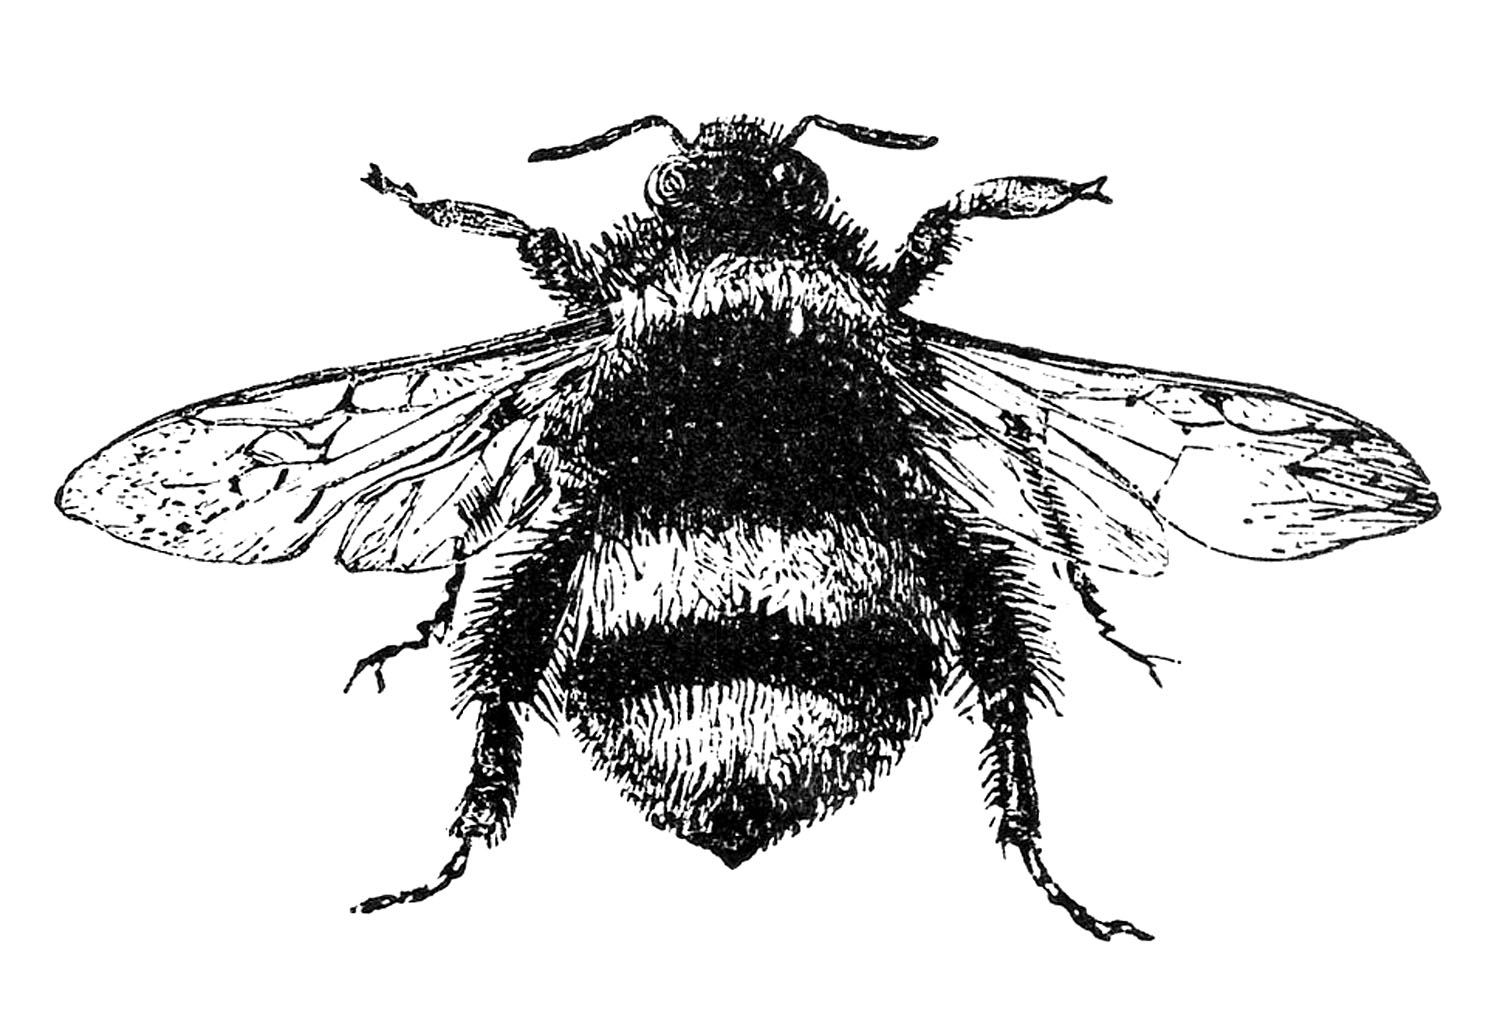
\includegraphics[scale=0.75]{img/bumblebee.jpg}
		\end{figure}
		\vspace{0.5cm}
		\Huge
		\textbf{\textsc{Metody Probabilistyczne Informatyki}}

		\vspace{0.5cm}
		\Large
		\textsc{Wybrane Dowody}

		\normalsize


		\line(1,0){330}

		\vspace{1cm}
		\textit{,,Tak teraz na to patrzę i myślę, czy ta nierówność nie powinna być w drugą stronę...''}
		\vspace{1cm}

		\textit{\textsc{Popełnione przez}}\\
		\vspace{5mm}

		\textbf{\textsc{
				Załatany Ponton \\
				V\\
				Nahtamatu\\
			}}

		\vfill

		Kraków \\
		Anno Domini 2025

	\end{center}

\end{titlepage}


\tableofcontents
\section*{Licencja}
\begin{figure}[h]
	\begin{minipage}[c]{0.25\textwidth}
		
\includegraphics[width=0.7\textwidth]{img/licencja.png}
	\end{minipage}\hfill
	\begin{minipage}[c]{0.75\textwidth}
		\caption*{
			Ten utwór jest dostępny na
			\href{https://creativecommons.org/licenses/by-sa/4.0/}{licencji Creative Commons Uznanie autorstwa
				na tych samych warunkach 4.0 Międzynarodowe.}
		}
	\end{minipage}
\end{figure}

% Remove the "Rozdział x" chapter headings, as we already number our chapters
\titleformat{\chapter}[display]{\normalfont\Huge\bfseries}{}{0pt}{\Huge}
\titlespacing*{\chapter}{0pt}{0pt}{20pt}

% Actual content
\mainmatter

\chapter{Wykład 1 (2025-10-03)}
 % Żeby nie było syfu to kolejne sekcje dodajemy do chapters/
% A potem includujemy za pomocą \input{chapters/...}

% Używamy \( \) i \[ \] zamiast dolarów -- tak jak się robi w LaTeXu


\documentclass[12pt, a4paper, polish, openany]{book}

% Please, let's familiarize ourselves with notatki.sty and tcs.sty so that we don't reinvent the wheel
\usepackage{notatki}
\fancyhead[L]{\textbf{\textit{MPI}}}

\begin{document}
% Front page and table of contents
\frontmatter

\input{titlepage}

\tableofcontents
\input{license}

% Remove the "Rozdział x" chapter headings, as we already number our chapters
\titleformat{\chapter}[display]{\normalfont\Huge\bfseries}{}{0pt}{\Huge}
\titlespacing*{\chapter}{0pt}{0pt}{20pt}

% Actual content
\mainmatter

\chapter{Wykład 1 (2025-10-03)}
\input{chapters/2025-10-03-lecture/main}

\chapter{Nagranie 1 (2025-10-04)}
\input{chapters/2025-10-04-recording/main}

\chapter{Wykład 2 (2025-10-10)}
\input{chapters/2025-10-10-lecture/main}

\chapter{Nagranie 2 (2025-10-10)}
\input{chapters/2025-10-10-recording/main}

\chapter{Wykład 3 (2025-10-17)}
\input{chapters/2025-10-17-lecture/main}

\end{document}


\chapter{Nagranie 1 (2025-10-04)}
 % Żeby nie było syfu to kolejne sekcje dodajemy do chapters/
% A potem includujemy za pomocą \input{chapters/...}

% Używamy \( \) i \[ \] zamiast dolarów -- tak jak się robi w LaTeXu


\documentclass[12pt, a4paper, polish, openany]{book}

% Please, let's familiarize ourselves with notatki.sty and tcs.sty so that we don't reinvent the wheel
\usepackage{notatki}
\fancyhead[L]{\textbf{\textit{MPI}}}

\begin{document}
% Front page and table of contents
\frontmatter

\input{titlepage}

\tableofcontents
\input{license}

% Remove the "Rozdział x" chapter headings, as we already number our chapters
\titleformat{\chapter}[display]{\normalfont\Huge\bfseries}{}{0pt}{\Huge}
\titlespacing*{\chapter}{0pt}{0pt}{20pt}

% Actual content
\mainmatter

\chapter{Wykład 1 (2025-10-03)}
\input{chapters/2025-10-03-lecture/main}

\chapter{Nagranie 1 (2025-10-04)}
\input{chapters/2025-10-04-recording/main}

\chapter{Wykład 2 (2025-10-10)}
\input{chapters/2025-10-10-lecture/main}

\chapter{Nagranie 2 (2025-10-10)}
\input{chapters/2025-10-10-recording/main}

\chapter{Wykład 3 (2025-10-17)}
\input{chapters/2025-10-17-lecture/main}

\end{document}


\chapter{Wykład 2 (2025-10-10)}
 % Żeby nie było syfu to kolejne sekcje dodajemy do chapters/
% A potem includujemy za pomocą \input{chapters/...}

% Używamy \( \) i \[ \] zamiast dolarów -- tak jak się robi w LaTeXu


\documentclass[12pt, a4paper, polish, openany]{book}

% Please, let's familiarize ourselves with notatki.sty and tcs.sty so that we don't reinvent the wheel
\usepackage{notatki}
\fancyhead[L]{\textbf{\textit{MPI}}}

\begin{document}
% Front page and table of contents
\frontmatter

\input{titlepage}

\tableofcontents
\input{license}

% Remove the "Rozdział x" chapter headings, as we already number our chapters
\titleformat{\chapter}[display]{\normalfont\Huge\bfseries}{}{0pt}{\Huge}
\titlespacing*{\chapter}{0pt}{0pt}{20pt}

% Actual content
\mainmatter

\chapter{Wykład 1 (2025-10-03)}
\input{chapters/2025-10-03-lecture/main}

\chapter{Nagranie 1 (2025-10-04)}
\input{chapters/2025-10-04-recording/main}

\chapter{Wykład 2 (2025-10-10)}
\input{chapters/2025-10-10-lecture/main}

\chapter{Nagranie 2 (2025-10-10)}
\input{chapters/2025-10-10-recording/main}

\chapter{Wykład 3 (2025-10-17)}
\input{chapters/2025-10-17-lecture/main}

\end{document}


\chapter{Nagranie 2 (2025-10-10)}
 % Żeby nie było syfu to kolejne sekcje dodajemy do chapters/
% A potem includujemy za pomocą \input{chapters/...}

% Używamy \( \) i \[ \] zamiast dolarów -- tak jak się robi w LaTeXu


\documentclass[12pt, a4paper, polish, openany]{book}

% Please, let's familiarize ourselves with notatki.sty and tcs.sty so that we don't reinvent the wheel
\usepackage{notatki}
\fancyhead[L]{\textbf{\textit{MPI}}}

\begin{document}
% Front page and table of contents
\frontmatter

\input{titlepage}

\tableofcontents
\input{license}

% Remove the "Rozdział x" chapter headings, as we already number our chapters
\titleformat{\chapter}[display]{\normalfont\Huge\bfseries}{}{0pt}{\Huge}
\titlespacing*{\chapter}{0pt}{0pt}{20pt}

% Actual content
\mainmatter

\chapter{Wykład 1 (2025-10-03)}
\input{chapters/2025-10-03-lecture/main}

\chapter{Nagranie 1 (2025-10-04)}
\input{chapters/2025-10-04-recording/main}

\chapter{Wykład 2 (2025-10-10)}
\input{chapters/2025-10-10-lecture/main}

\chapter{Nagranie 2 (2025-10-10)}
\input{chapters/2025-10-10-recording/main}

\chapter{Wykład 3 (2025-10-17)}
\input{chapters/2025-10-17-lecture/main}

\end{document}


\chapter{Wykład 3 (2025-10-17)}
 % Żeby nie było syfu to kolejne sekcje dodajemy do chapters/
% A potem includujemy za pomocą \input{chapters/...}

% Używamy \( \) i \[ \] zamiast dolarów -- tak jak się robi w LaTeXu


\documentclass[12pt, a4paper, polish, openany]{book}

% Please, let's familiarize ourselves with notatki.sty and tcs.sty so that we don't reinvent the wheel
\usepackage{notatki}
\fancyhead[L]{\textbf{\textit{MPI}}}

\begin{document}
% Front page and table of contents
\frontmatter

\input{titlepage}

\tableofcontents
\input{license}

% Remove the "Rozdział x" chapter headings, as we already number our chapters
\titleformat{\chapter}[display]{\normalfont\Huge\bfseries}{}{0pt}{\Huge}
\titlespacing*{\chapter}{0pt}{0pt}{20pt}

% Actual content
\mainmatter

\chapter{Wykład 1 (2025-10-03)}
\input{chapters/2025-10-03-lecture/main}

\chapter{Nagranie 1 (2025-10-04)}
\input{chapters/2025-10-04-recording/main}

\chapter{Wykład 2 (2025-10-10)}
\input{chapters/2025-10-10-lecture/main}

\chapter{Nagranie 2 (2025-10-10)}
\input{chapters/2025-10-10-recording/main}

\chapter{Wykład 3 (2025-10-17)}
\input{chapters/2025-10-17-lecture/main}

\end{document}


\end{document}


\chapter{Wykład 2 (2025-10-10)}
 % Żeby nie było syfu to kolejne sekcje dodajemy do chapters/
% A potem includujemy za pomocą \input{chapters/...}

% Używamy \( \) i \[ \] zamiast dolarów -- tak jak się robi w LaTeXu


\documentclass[12pt, a4paper, polish, openany]{book}

% Please, let's familiarize ourselves with notatki.sty and tcs.sty so that we don't reinvent the wheel
\usepackage{notatki}
\fancyhead[L]{\textbf{\textit{MPI}}}

\begin{document}
% Front page and table of contents
\frontmatter

\begin{titlepage}

	\begin{center}
		\begin{figure}[h]
			\centering
			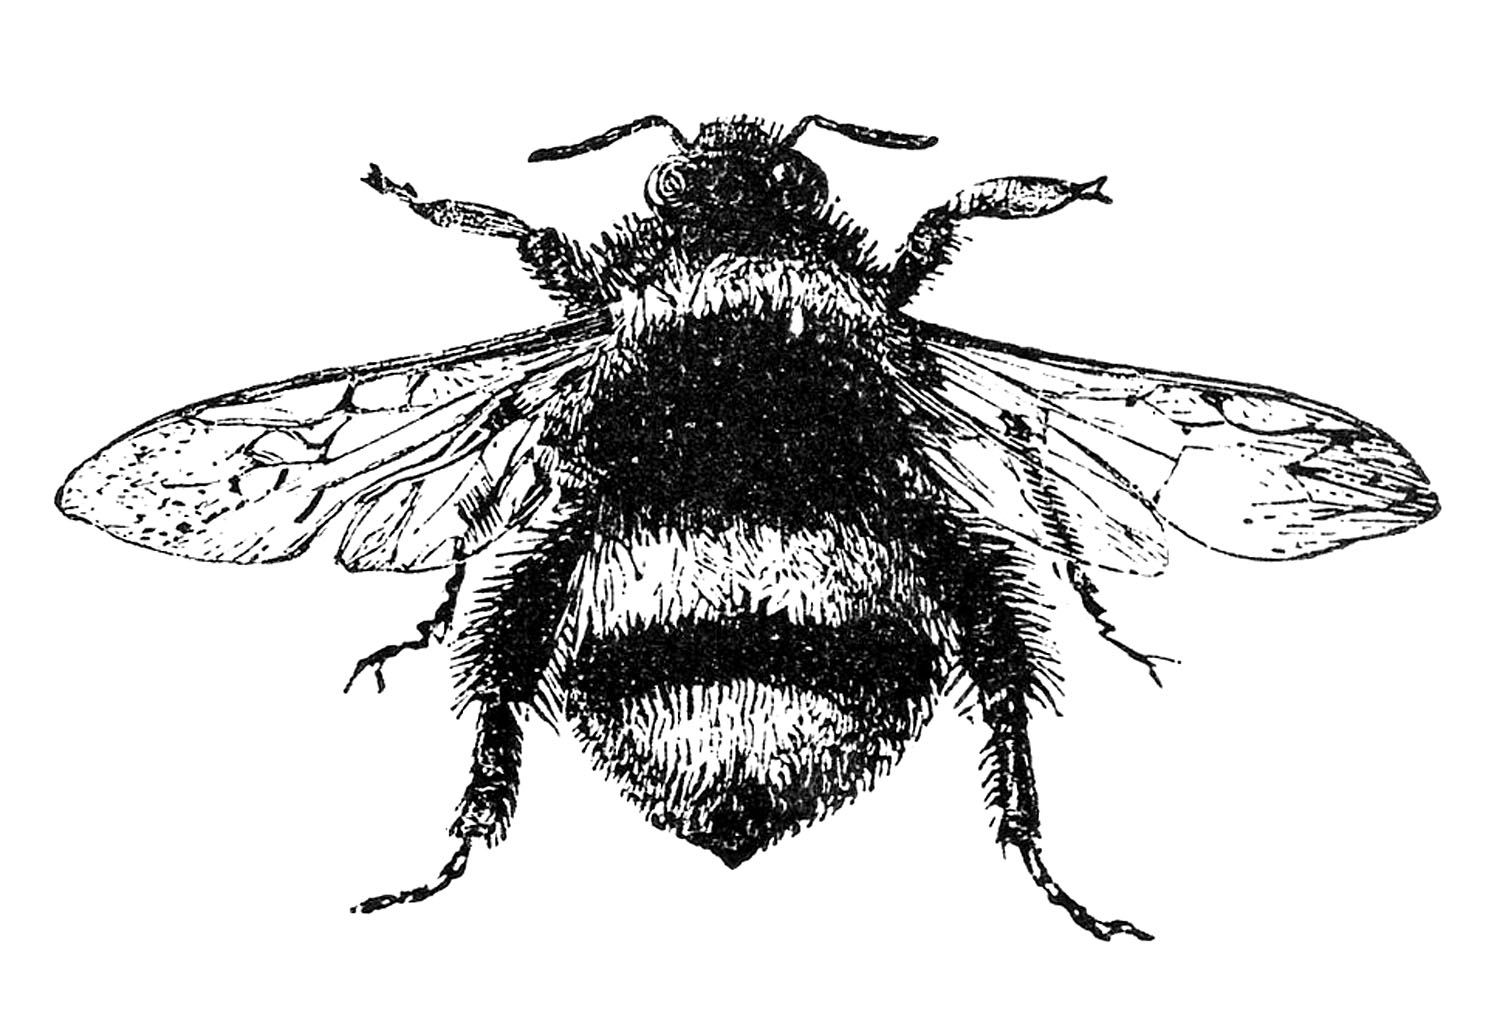
\includegraphics[scale=0.75]{img/bumblebee.jpg}
		\end{figure}
		\vspace{0.5cm}
		\Huge
		\textbf{\textsc{Metody Probabilistyczne Informatyki}}

		\vspace{0.5cm}
		\Large
		\textsc{Wybrane Dowody}

		\normalsize


		\line(1,0){330}

		\vspace{1cm}
		\textit{,,Tak teraz na to patrzę i myślę, czy ta nierówność nie powinna być w drugą stronę...''}
		\vspace{1cm}

		\textit{\textsc{Popełnione przez}}\\
		\vspace{5mm}

		\textbf{\textsc{
				Załatany Ponton \\
				V\\
				Nahtamatu\\
			}}

		\vfill

		Kraków \\
		Anno Domini 2025

	\end{center}

\end{titlepage}


\tableofcontents
\section*{Licencja}
\begin{figure}[h]
	\begin{minipage}[c]{0.25\textwidth}
		
\includegraphics[width=0.7\textwidth]{img/licencja.png}
	\end{minipage}\hfill
	\begin{minipage}[c]{0.75\textwidth}
		\caption*{
			Ten utwór jest dostępny na
			\href{https://creativecommons.org/licenses/by-sa/4.0/}{licencji Creative Commons Uznanie autorstwa
				na tych samych warunkach 4.0 Międzynarodowe.}
		}
	\end{minipage}
\end{figure}

% Remove the "Rozdział x" chapter headings, as we already number our chapters
\titleformat{\chapter}[display]{\normalfont\Huge\bfseries}{}{0pt}{\Huge}
\titlespacing*{\chapter}{0pt}{0pt}{20pt}

% Actual content
\mainmatter

\chapter{Wykład 1 (2025-10-03)}
 % Żeby nie było syfu to kolejne sekcje dodajemy do chapters/
% A potem includujemy za pomocą \input{chapters/...}

% Używamy \( \) i \[ \] zamiast dolarów -- tak jak się robi w LaTeXu


\documentclass[12pt, a4paper, polish, openany]{book}

% Please, let's familiarize ourselves with notatki.sty and tcs.sty so that we don't reinvent the wheel
\usepackage{notatki}
\fancyhead[L]{\textbf{\textit{MPI}}}

\begin{document}
% Front page and table of contents
\frontmatter

\input{titlepage}

\tableofcontents
\input{license}

% Remove the "Rozdział x" chapter headings, as we already number our chapters
\titleformat{\chapter}[display]{\normalfont\Huge\bfseries}{}{0pt}{\Huge}
\titlespacing*{\chapter}{0pt}{0pt}{20pt}

% Actual content
\mainmatter

\chapter{Wykład 1 (2025-10-03)}
\input{chapters/2025-10-03-lecture/main}

\chapter{Nagranie 1 (2025-10-04)}
\input{chapters/2025-10-04-recording/main}

\chapter{Wykład 2 (2025-10-10)}
\input{chapters/2025-10-10-lecture/main}

\chapter{Nagranie 2 (2025-10-10)}
\input{chapters/2025-10-10-recording/main}

\chapter{Wykład 3 (2025-10-17)}
\input{chapters/2025-10-17-lecture/main}

\end{document}


\chapter{Nagranie 1 (2025-10-04)}
 % Żeby nie było syfu to kolejne sekcje dodajemy do chapters/
% A potem includujemy za pomocą \input{chapters/...}

% Używamy \( \) i \[ \] zamiast dolarów -- tak jak się robi w LaTeXu


\documentclass[12pt, a4paper, polish, openany]{book}

% Please, let's familiarize ourselves with notatki.sty and tcs.sty so that we don't reinvent the wheel
\usepackage{notatki}
\fancyhead[L]{\textbf{\textit{MPI}}}

\begin{document}
% Front page and table of contents
\frontmatter

\input{titlepage}

\tableofcontents
\input{license}

% Remove the "Rozdział x" chapter headings, as we already number our chapters
\titleformat{\chapter}[display]{\normalfont\Huge\bfseries}{}{0pt}{\Huge}
\titlespacing*{\chapter}{0pt}{0pt}{20pt}

% Actual content
\mainmatter

\chapter{Wykład 1 (2025-10-03)}
\input{chapters/2025-10-03-lecture/main}

\chapter{Nagranie 1 (2025-10-04)}
\input{chapters/2025-10-04-recording/main}

\chapter{Wykład 2 (2025-10-10)}
\input{chapters/2025-10-10-lecture/main}

\chapter{Nagranie 2 (2025-10-10)}
\input{chapters/2025-10-10-recording/main}

\chapter{Wykład 3 (2025-10-17)}
\input{chapters/2025-10-17-lecture/main}

\end{document}


\chapter{Wykład 2 (2025-10-10)}
 % Żeby nie było syfu to kolejne sekcje dodajemy do chapters/
% A potem includujemy za pomocą \input{chapters/...}

% Używamy \( \) i \[ \] zamiast dolarów -- tak jak się robi w LaTeXu


\documentclass[12pt, a4paper, polish, openany]{book}

% Please, let's familiarize ourselves with notatki.sty and tcs.sty so that we don't reinvent the wheel
\usepackage{notatki}
\fancyhead[L]{\textbf{\textit{MPI}}}

\begin{document}
% Front page and table of contents
\frontmatter

\input{titlepage}

\tableofcontents
\input{license}

% Remove the "Rozdział x" chapter headings, as we already number our chapters
\titleformat{\chapter}[display]{\normalfont\Huge\bfseries}{}{0pt}{\Huge}
\titlespacing*{\chapter}{0pt}{0pt}{20pt}

% Actual content
\mainmatter

\chapter{Wykład 1 (2025-10-03)}
\input{chapters/2025-10-03-lecture/main}

\chapter{Nagranie 1 (2025-10-04)}
\input{chapters/2025-10-04-recording/main}

\chapter{Wykład 2 (2025-10-10)}
\input{chapters/2025-10-10-lecture/main}

\chapter{Nagranie 2 (2025-10-10)}
\input{chapters/2025-10-10-recording/main}

\chapter{Wykład 3 (2025-10-17)}
\input{chapters/2025-10-17-lecture/main}

\end{document}


\chapter{Nagranie 2 (2025-10-10)}
 % Żeby nie było syfu to kolejne sekcje dodajemy do chapters/
% A potem includujemy za pomocą \input{chapters/...}

% Używamy \( \) i \[ \] zamiast dolarów -- tak jak się robi w LaTeXu


\documentclass[12pt, a4paper, polish, openany]{book}

% Please, let's familiarize ourselves with notatki.sty and tcs.sty so that we don't reinvent the wheel
\usepackage{notatki}
\fancyhead[L]{\textbf{\textit{MPI}}}

\begin{document}
% Front page and table of contents
\frontmatter

\input{titlepage}

\tableofcontents
\input{license}

% Remove the "Rozdział x" chapter headings, as we already number our chapters
\titleformat{\chapter}[display]{\normalfont\Huge\bfseries}{}{0pt}{\Huge}
\titlespacing*{\chapter}{0pt}{0pt}{20pt}

% Actual content
\mainmatter

\chapter{Wykład 1 (2025-10-03)}
\input{chapters/2025-10-03-lecture/main}

\chapter{Nagranie 1 (2025-10-04)}
\input{chapters/2025-10-04-recording/main}

\chapter{Wykład 2 (2025-10-10)}
\input{chapters/2025-10-10-lecture/main}

\chapter{Nagranie 2 (2025-10-10)}
\input{chapters/2025-10-10-recording/main}

\chapter{Wykład 3 (2025-10-17)}
\input{chapters/2025-10-17-lecture/main}

\end{document}


\chapter{Wykład 3 (2025-10-17)}
 % Żeby nie było syfu to kolejne sekcje dodajemy do chapters/
% A potem includujemy za pomocą \input{chapters/...}

% Używamy \( \) i \[ \] zamiast dolarów -- tak jak się robi w LaTeXu


\documentclass[12pt, a4paper, polish, openany]{book}

% Please, let's familiarize ourselves with notatki.sty and tcs.sty so that we don't reinvent the wheel
\usepackage{notatki}
\fancyhead[L]{\textbf{\textit{MPI}}}

\begin{document}
% Front page and table of contents
\frontmatter

\input{titlepage}

\tableofcontents
\input{license}

% Remove the "Rozdział x" chapter headings, as we already number our chapters
\titleformat{\chapter}[display]{\normalfont\Huge\bfseries}{}{0pt}{\Huge}
\titlespacing*{\chapter}{0pt}{0pt}{20pt}

% Actual content
\mainmatter

\chapter{Wykład 1 (2025-10-03)}
\input{chapters/2025-10-03-lecture/main}

\chapter{Nagranie 1 (2025-10-04)}
\input{chapters/2025-10-04-recording/main}

\chapter{Wykład 2 (2025-10-10)}
\input{chapters/2025-10-10-lecture/main}

\chapter{Nagranie 2 (2025-10-10)}
\input{chapters/2025-10-10-recording/main}

\chapter{Wykład 3 (2025-10-17)}
\input{chapters/2025-10-17-lecture/main}

\end{document}


\end{document}


\chapter{Nagranie 2 (2025-10-10)}
 % Żeby nie było syfu to kolejne sekcje dodajemy do chapters/
% A potem includujemy za pomocą \input{chapters/...}

% Używamy \( \) i \[ \] zamiast dolarów -- tak jak się robi w LaTeXu


\documentclass[12pt, a4paper, polish, openany]{book}

% Please, let's familiarize ourselves with notatki.sty and tcs.sty so that we don't reinvent the wheel
\usepackage{notatki}
\fancyhead[L]{\textbf{\textit{MPI}}}

\begin{document}
% Front page and table of contents
\frontmatter

\begin{titlepage}

	\begin{center}
		\begin{figure}[h]
			\centering
			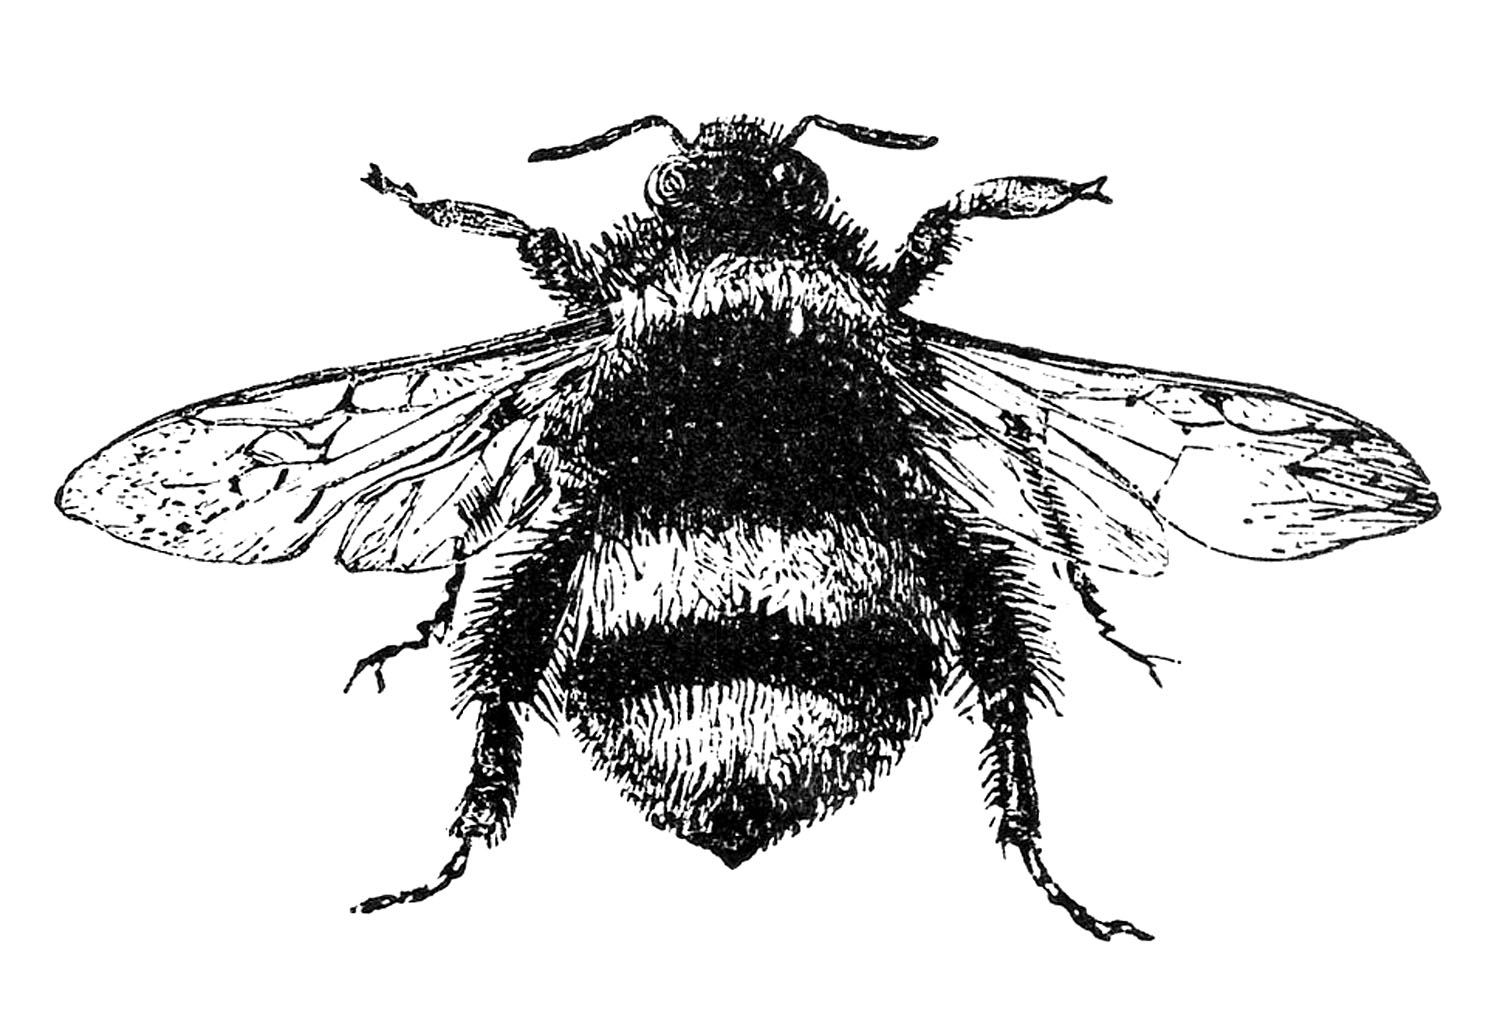
\includegraphics[scale=0.75]{img/bumblebee.jpg}
		\end{figure}
		\vspace{0.5cm}
		\Huge
		\textbf{\textsc{Metody Probabilistyczne Informatyki}}

		\vspace{0.5cm}
		\Large
		\textsc{Wybrane Dowody}

		\normalsize


		\line(1,0){330}

		\vspace{1cm}
		\textit{,,Tak teraz na to patrzę i myślę, czy ta nierówność nie powinna być w drugą stronę...''}
		\vspace{1cm}

		\textit{\textsc{Popełnione przez}}\\
		\vspace{5mm}

		\textbf{\textsc{
				Załatany Ponton \\
				V\\
				Nahtamatu\\
			}}

		\vfill

		Kraków \\
		Anno Domini 2025

	\end{center}

\end{titlepage}


\tableofcontents
\section*{Licencja}
\begin{figure}[h]
	\begin{minipage}[c]{0.25\textwidth}
		
\includegraphics[width=0.7\textwidth]{img/licencja.png}
	\end{minipage}\hfill
	\begin{minipage}[c]{0.75\textwidth}
		\caption*{
			Ten utwór jest dostępny na
			\href{https://creativecommons.org/licenses/by-sa/4.0/}{licencji Creative Commons Uznanie autorstwa
				na tych samych warunkach 4.0 Międzynarodowe.}
		}
	\end{minipage}
\end{figure}

% Remove the "Rozdział x" chapter headings, as we already number our chapters
\titleformat{\chapter}[display]{\normalfont\Huge\bfseries}{}{0pt}{\Huge}
\titlespacing*{\chapter}{0pt}{0pt}{20pt}

% Actual content
\mainmatter

\chapter{Wykład 1 (2025-10-03)}
 % Żeby nie było syfu to kolejne sekcje dodajemy do chapters/
% A potem includujemy za pomocą \input{chapters/...}

% Używamy \( \) i \[ \] zamiast dolarów -- tak jak się robi w LaTeXu


\documentclass[12pt, a4paper, polish, openany]{book}

% Please, let's familiarize ourselves with notatki.sty and tcs.sty so that we don't reinvent the wheel
\usepackage{notatki}
\fancyhead[L]{\textbf{\textit{MPI}}}

\begin{document}
% Front page and table of contents
\frontmatter

\input{titlepage}

\tableofcontents
\input{license}

% Remove the "Rozdział x" chapter headings, as we already number our chapters
\titleformat{\chapter}[display]{\normalfont\Huge\bfseries}{}{0pt}{\Huge}
\titlespacing*{\chapter}{0pt}{0pt}{20pt}

% Actual content
\mainmatter

\chapter{Wykład 1 (2025-10-03)}
\input{chapters/2025-10-03-lecture/main}

\chapter{Nagranie 1 (2025-10-04)}
\input{chapters/2025-10-04-recording/main}

\chapter{Wykład 2 (2025-10-10)}
\input{chapters/2025-10-10-lecture/main}

\chapter{Nagranie 2 (2025-10-10)}
\input{chapters/2025-10-10-recording/main}

\chapter{Wykład 3 (2025-10-17)}
\input{chapters/2025-10-17-lecture/main}

\end{document}


\chapter{Nagranie 1 (2025-10-04)}
 % Żeby nie było syfu to kolejne sekcje dodajemy do chapters/
% A potem includujemy za pomocą \input{chapters/...}

% Używamy \( \) i \[ \] zamiast dolarów -- tak jak się robi w LaTeXu


\documentclass[12pt, a4paper, polish, openany]{book}

% Please, let's familiarize ourselves with notatki.sty and tcs.sty so that we don't reinvent the wheel
\usepackage{notatki}
\fancyhead[L]{\textbf{\textit{MPI}}}

\begin{document}
% Front page and table of contents
\frontmatter

\input{titlepage}

\tableofcontents
\input{license}

% Remove the "Rozdział x" chapter headings, as we already number our chapters
\titleformat{\chapter}[display]{\normalfont\Huge\bfseries}{}{0pt}{\Huge}
\titlespacing*{\chapter}{0pt}{0pt}{20pt}

% Actual content
\mainmatter

\chapter{Wykład 1 (2025-10-03)}
\input{chapters/2025-10-03-lecture/main}

\chapter{Nagranie 1 (2025-10-04)}
\input{chapters/2025-10-04-recording/main}

\chapter{Wykład 2 (2025-10-10)}
\input{chapters/2025-10-10-lecture/main}

\chapter{Nagranie 2 (2025-10-10)}
\input{chapters/2025-10-10-recording/main}

\chapter{Wykład 3 (2025-10-17)}
\input{chapters/2025-10-17-lecture/main}

\end{document}


\chapter{Wykład 2 (2025-10-10)}
 % Żeby nie było syfu to kolejne sekcje dodajemy do chapters/
% A potem includujemy za pomocą \input{chapters/...}

% Używamy \( \) i \[ \] zamiast dolarów -- tak jak się robi w LaTeXu


\documentclass[12pt, a4paper, polish, openany]{book}

% Please, let's familiarize ourselves with notatki.sty and tcs.sty so that we don't reinvent the wheel
\usepackage{notatki}
\fancyhead[L]{\textbf{\textit{MPI}}}

\begin{document}
% Front page and table of contents
\frontmatter

\input{titlepage}

\tableofcontents
\input{license}

% Remove the "Rozdział x" chapter headings, as we already number our chapters
\titleformat{\chapter}[display]{\normalfont\Huge\bfseries}{}{0pt}{\Huge}
\titlespacing*{\chapter}{0pt}{0pt}{20pt}

% Actual content
\mainmatter

\chapter{Wykład 1 (2025-10-03)}
\input{chapters/2025-10-03-lecture/main}

\chapter{Nagranie 1 (2025-10-04)}
\input{chapters/2025-10-04-recording/main}

\chapter{Wykład 2 (2025-10-10)}
\input{chapters/2025-10-10-lecture/main}

\chapter{Nagranie 2 (2025-10-10)}
\input{chapters/2025-10-10-recording/main}

\chapter{Wykład 3 (2025-10-17)}
\input{chapters/2025-10-17-lecture/main}

\end{document}


\chapter{Nagranie 2 (2025-10-10)}
 % Żeby nie było syfu to kolejne sekcje dodajemy do chapters/
% A potem includujemy za pomocą \input{chapters/...}

% Używamy \( \) i \[ \] zamiast dolarów -- tak jak się robi w LaTeXu


\documentclass[12pt, a4paper, polish, openany]{book}

% Please, let's familiarize ourselves with notatki.sty and tcs.sty so that we don't reinvent the wheel
\usepackage{notatki}
\fancyhead[L]{\textbf{\textit{MPI}}}

\begin{document}
% Front page and table of contents
\frontmatter

\input{titlepage}

\tableofcontents
\input{license}

% Remove the "Rozdział x" chapter headings, as we already number our chapters
\titleformat{\chapter}[display]{\normalfont\Huge\bfseries}{}{0pt}{\Huge}
\titlespacing*{\chapter}{0pt}{0pt}{20pt}

% Actual content
\mainmatter

\chapter{Wykład 1 (2025-10-03)}
\input{chapters/2025-10-03-lecture/main}

\chapter{Nagranie 1 (2025-10-04)}
\input{chapters/2025-10-04-recording/main}

\chapter{Wykład 2 (2025-10-10)}
\input{chapters/2025-10-10-lecture/main}

\chapter{Nagranie 2 (2025-10-10)}
\input{chapters/2025-10-10-recording/main}

\chapter{Wykład 3 (2025-10-17)}
\input{chapters/2025-10-17-lecture/main}

\end{document}


\chapter{Wykład 3 (2025-10-17)}
 % Żeby nie było syfu to kolejne sekcje dodajemy do chapters/
% A potem includujemy za pomocą \input{chapters/...}

% Używamy \( \) i \[ \] zamiast dolarów -- tak jak się robi w LaTeXu


\documentclass[12pt, a4paper, polish, openany]{book}

% Please, let's familiarize ourselves with notatki.sty and tcs.sty so that we don't reinvent the wheel
\usepackage{notatki}
\fancyhead[L]{\textbf{\textit{MPI}}}

\begin{document}
% Front page and table of contents
\frontmatter

\input{titlepage}

\tableofcontents
\input{license}

% Remove the "Rozdział x" chapter headings, as we already number our chapters
\titleformat{\chapter}[display]{\normalfont\Huge\bfseries}{}{0pt}{\Huge}
\titlespacing*{\chapter}{0pt}{0pt}{20pt}

% Actual content
\mainmatter

\chapter{Wykład 1 (2025-10-03)}
\input{chapters/2025-10-03-lecture/main}

\chapter{Nagranie 1 (2025-10-04)}
\input{chapters/2025-10-04-recording/main}

\chapter{Wykład 2 (2025-10-10)}
\input{chapters/2025-10-10-lecture/main}

\chapter{Nagranie 2 (2025-10-10)}
\input{chapters/2025-10-10-recording/main}

\chapter{Wykład 3 (2025-10-17)}
\input{chapters/2025-10-17-lecture/main}

\end{document}


\end{document}


\chapter{Wykład 3 (2025-10-17)}
 % Żeby nie było syfu to kolejne sekcje dodajemy do chapters/
% A potem includujemy za pomocą \input{chapters/...}

% Używamy \( \) i \[ \] zamiast dolarów -- tak jak się robi w LaTeXu


\documentclass[12pt, a4paper, polish, openany]{book}

% Please, let's familiarize ourselves with notatki.sty and tcs.sty so that we don't reinvent the wheel
\usepackage{notatki}
\fancyhead[L]{\textbf{\textit{MPI}}}

\begin{document}
% Front page and table of contents
\frontmatter

\begin{titlepage}

	\begin{center}
		\begin{figure}[h]
			\centering
			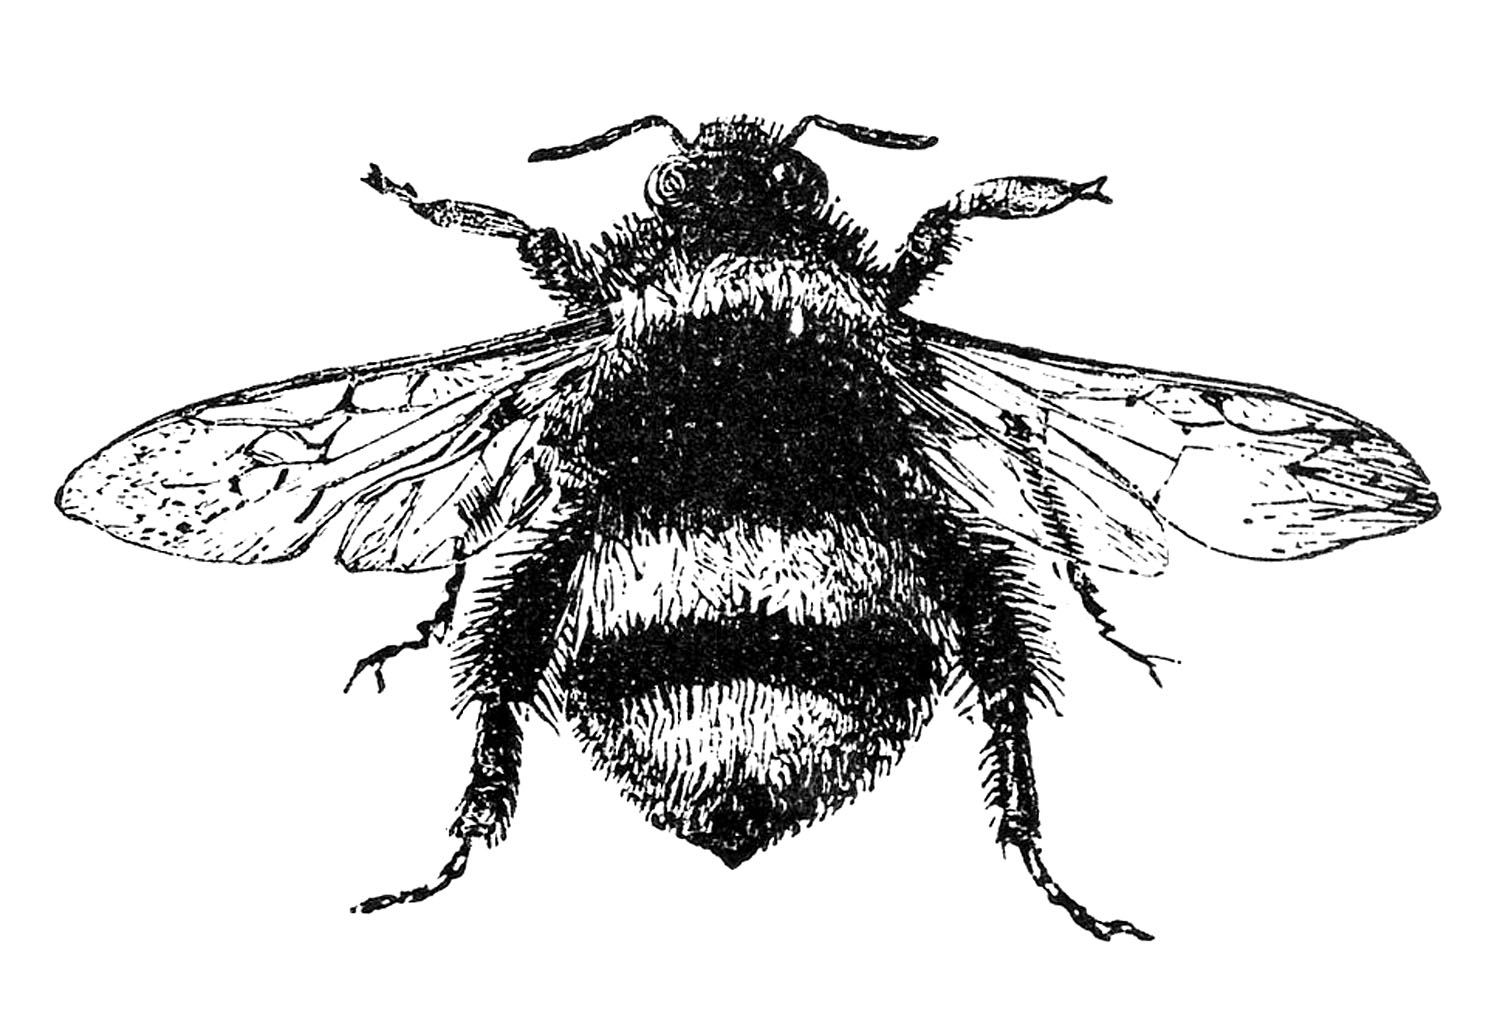
\includegraphics[scale=0.75]{img/bumblebee.jpg}
		\end{figure}
		\vspace{0.5cm}
		\Huge
		\textbf{\textsc{Metody Probabilistyczne Informatyki}}

		\vspace{0.5cm}
		\Large
		\textsc{Wybrane Dowody}

		\normalsize


		\line(1,0){330}

		\vspace{1cm}
		\textit{,,Tak teraz na to patrzę i myślę, czy ta nierówność nie powinna być w drugą stronę...''}
		\vspace{1cm}

		\textit{\textsc{Popełnione przez}}\\
		\vspace{5mm}

		\textbf{\textsc{
				Załatany Ponton \\
				V\\
				Nahtamatu\\
			}}

		\vfill

		Kraków \\
		Anno Domini 2025

	\end{center}

\end{titlepage}


\tableofcontents
\section*{Licencja}
\begin{figure}[h]
	\begin{minipage}[c]{0.25\textwidth}
		
\includegraphics[width=0.7\textwidth]{img/licencja.png}
	\end{minipage}\hfill
	\begin{minipage}[c]{0.75\textwidth}
		\caption*{
			Ten utwór jest dostępny na
			\href{https://creativecommons.org/licenses/by-sa/4.0/}{licencji Creative Commons Uznanie autorstwa
				na tych samych warunkach 4.0 Międzynarodowe.}
		}
	\end{minipage}
\end{figure}

% Remove the "Rozdział x" chapter headings, as we already number our chapters
\titleformat{\chapter}[display]{\normalfont\Huge\bfseries}{}{0pt}{\Huge}
\titlespacing*{\chapter}{0pt}{0pt}{20pt}

% Actual content
\mainmatter

\chapter{Wykład 1 (2025-10-03)}
 % Żeby nie było syfu to kolejne sekcje dodajemy do chapters/
% A potem includujemy za pomocą \input{chapters/...}

% Używamy \( \) i \[ \] zamiast dolarów -- tak jak się robi w LaTeXu


\documentclass[12pt, a4paper, polish, openany]{book}

% Please, let's familiarize ourselves with notatki.sty and tcs.sty so that we don't reinvent the wheel
\usepackage{notatki}
\fancyhead[L]{\textbf{\textit{MPI}}}

\begin{document}
% Front page and table of contents
\frontmatter

\input{titlepage}

\tableofcontents
\input{license}

% Remove the "Rozdział x" chapter headings, as we already number our chapters
\titleformat{\chapter}[display]{\normalfont\Huge\bfseries}{}{0pt}{\Huge}
\titlespacing*{\chapter}{0pt}{0pt}{20pt}

% Actual content
\mainmatter

\chapter{Wykład 1 (2025-10-03)}
\input{chapters/2025-10-03-lecture/main}

\chapter{Nagranie 1 (2025-10-04)}
\input{chapters/2025-10-04-recording/main}

\chapter{Wykład 2 (2025-10-10)}
\input{chapters/2025-10-10-lecture/main}

\chapter{Nagranie 2 (2025-10-10)}
\input{chapters/2025-10-10-recording/main}

\chapter{Wykład 3 (2025-10-17)}
\input{chapters/2025-10-17-lecture/main}

\end{document}


\chapter{Nagranie 1 (2025-10-04)}
 % Żeby nie było syfu to kolejne sekcje dodajemy do chapters/
% A potem includujemy za pomocą \input{chapters/...}

% Używamy \( \) i \[ \] zamiast dolarów -- tak jak się robi w LaTeXu


\documentclass[12pt, a4paper, polish, openany]{book}

% Please, let's familiarize ourselves with notatki.sty and tcs.sty so that we don't reinvent the wheel
\usepackage{notatki}
\fancyhead[L]{\textbf{\textit{MPI}}}

\begin{document}
% Front page and table of contents
\frontmatter

\input{titlepage}

\tableofcontents
\input{license}

% Remove the "Rozdział x" chapter headings, as we already number our chapters
\titleformat{\chapter}[display]{\normalfont\Huge\bfseries}{}{0pt}{\Huge}
\titlespacing*{\chapter}{0pt}{0pt}{20pt}

% Actual content
\mainmatter

\chapter{Wykład 1 (2025-10-03)}
\input{chapters/2025-10-03-lecture/main}

\chapter{Nagranie 1 (2025-10-04)}
\input{chapters/2025-10-04-recording/main}

\chapter{Wykład 2 (2025-10-10)}
\input{chapters/2025-10-10-lecture/main}

\chapter{Nagranie 2 (2025-10-10)}
\input{chapters/2025-10-10-recording/main}

\chapter{Wykład 3 (2025-10-17)}
\input{chapters/2025-10-17-lecture/main}

\end{document}


\chapter{Wykład 2 (2025-10-10)}
 % Żeby nie było syfu to kolejne sekcje dodajemy do chapters/
% A potem includujemy za pomocą \input{chapters/...}

% Używamy \( \) i \[ \] zamiast dolarów -- tak jak się robi w LaTeXu


\documentclass[12pt, a4paper, polish, openany]{book}

% Please, let's familiarize ourselves with notatki.sty and tcs.sty so that we don't reinvent the wheel
\usepackage{notatki}
\fancyhead[L]{\textbf{\textit{MPI}}}

\begin{document}
% Front page and table of contents
\frontmatter

\input{titlepage}

\tableofcontents
\input{license}

% Remove the "Rozdział x" chapter headings, as we already number our chapters
\titleformat{\chapter}[display]{\normalfont\Huge\bfseries}{}{0pt}{\Huge}
\titlespacing*{\chapter}{0pt}{0pt}{20pt}

% Actual content
\mainmatter

\chapter{Wykład 1 (2025-10-03)}
\input{chapters/2025-10-03-lecture/main}

\chapter{Nagranie 1 (2025-10-04)}
\input{chapters/2025-10-04-recording/main}

\chapter{Wykład 2 (2025-10-10)}
\input{chapters/2025-10-10-lecture/main}

\chapter{Nagranie 2 (2025-10-10)}
\input{chapters/2025-10-10-recording/main}

\chapter{Wykład 3 (2025-10-17)}
\input{chapters/2025-10-17-lecture/main}

\end{document}


\chapter{Nagranie 2 (2025-10-10)}
 % Żeby nie było syfu to kolejne sekcje dodajemy do chapters/
% A potem includujemy za pomocą \input{chapters/...}

% Używamy \( \) i \[ \] zamiast dolarów -- tak jak się robi w LaTeXu


\documentclass[12pt, a4paper, polish, openany]{book}

% Please, let's familiarize ourselves with notatki.sty and tcs.sty so that we don't reinvent the wheel
\usepackage{notatki}
\fancyhead[L]{\textbf{\textit{MPI}}}

\begin{document}
% Front page and table of contents
\frontmatter

\input{titlepage}

\tableofcontents
\input{license}

% Remove the "Rozdział x" chapter headings, as we already number our chapters
\titleformat{\chapter}[display]{\normalfont\Huge\bfseries}{}{0pt}{\Huge}
\titlespacing*{\chapter}{0pt}{0pt}{20pt}

% Actual content
\mainmatter

\chapter{Wykład 1 (2025-10-03)}
\input{chapters/2025-10-03-lecture/main}

\chapter{Nagranie 1 (2025-10-04)}
\input{chapters/2025-10-04-recording/main}

\chapter{Wykład 2 (2025-10-10)}
\input{chapters/2025-10-10-lecture/main}

\chapter{Nagranie 2 (2025-10-10)}
\input{chapters/2025-10-10-recording/main}

\chapter{Wykład 3 (2025-10-17)}
\input{chapters/2025-10-17-lecture/main}

\end{document}


\chapter{Wykład 3 (2025-10-17)}
 % Żeby nie było syfu to kolejne sekcje dodajemy do chapters/
% A potem includujemy za pomocą \input{chapters/...}

% Używamy \( \) i \[ \] zamiast dolarów -- tak jak się robi w LaTeXu


\documentclass[12pt, a4paper, polish, openany]{book}

% Please, let's familiarize ourselves with notatki.sty and tcs.sty so that we don't reinvent the wheel
\usepackage{notatki}
\fancyhead[L]{\textbf{\textit{MPI}}}

\begin{document}
% Front page and table of contents
\frontmatter

\input{titlepage}

\tableofcontents
\input{license}

% Remove the "Rozdział x" chapter headings, as we already number our chapters
\titleformat{\chapter}[display]{\normalfont\Huge\bfseries}{}{0pt}{\Huge}
\titlespacing*{\chapter}{0pt}{0pt}{20pt}

% Actual content
\mainmatter

\chapter{Wykład 1 (2025-10-03)}
\input{chapters/2025-10-03-lecture/main}

\chapter{Nagranie 1 (2025-10-04)}
\input{chapters/2025-10-04-recording/main}

\chapter{Wykład 2 (2025-10-10)}
\input{chapters/2025-10-10-lecture/main}

\chapter{Nagranie 2 (2025-10-10)}
\input{chapters/2025-10-10-recording/main}

\chapter{Wykład 3 (2025-10-17)}
\input{chapters/2025-10-17-lecture/main}

\end{document}


\end{document}


\end{document}


\realsection{Funkcje tworzące. Wyznaczanie liczb Fibonacciego za pomocą funkcji tworzących}

\epigraph{I can elaborate: zrobiłam zadanka, zobaczyłam tworzące, stwierdziłam, że chce mi się spać, poszłam sobie}{\textit{Studentka TCSu o zadaniach z funkcji tworzących na kolokwium}}
\subsection{Rozkład na ułamki proste}
To nie jest formalny dowód ani formalna własność ani nic, bardziej schemat postępowania przy rozkładzie na ułamki proste. Sam dowód tego, że rozkład na ułamki proste istnieje, to \textit{sprowadź do wspólnego mianownika i zobacz co Ci wyszło}.
Jeżeli \(deg(P(x)) < deg(Q(x))\) i \(Q(x) = (x-a)^n \cdot (x-b)^k\) to:
\begin{equation*}
	\frac{P(x)}{Q(x)} = \frac{P(x)}{(x-a)^n \cdot (x-b)^k} = \frac{A_1}{x-a} + \frac{A_2}{(x-a)^2} + \dots + \frac{A_n}{(x-a)^n} + \frac{B_1}{x-b} + \frac{B_2}{(x-b)^2} + \dots + \frac{B_k}{(x-b)^k}
\end{equation*}

Oczywiście ten schemat można rozszerzać na więcej śmiesznych rzeczy w mianowniku, ale chyba widać o co chodzi.


\realsubsection{Wzór Bineta}
\begin{theorem}[Wzór Bineta]
	\begin{equation}
		f_n = \frac{1}{\sqrt{5}} \cdot \left( \left(\frac{1 + \sqrt{5}}{2}\right)^{n} - \left(\frac{1 - \sqrt{5}}{2}\right)^{n} \right)
	\end{equation}
\end{theorem}

\begin{proof}
	Rozpisujemy sobie funkcję tworzącą ciągu \(f_n\):

	\begin{equation*}
		F(x) = f_0 + f_1 \cdot x + f_2 \cdot x^2 + f_3 \cdot x^3 \dots =
	\end{equation*}
	\begin{equation*}
		= f_0 + f_1 \cdot x + (f_0 + f_1) \cdot x^2 + (f_1 + f_2) \cdot x^3 + \dots =
	\end{equation*}
	\begin{equation*}
		= f_0 + f_1 \cdot x + f_0 \cdot x^2 + f_1 \cdot x^2 + f_1 \cdot x^3 + f_2 \cdot x^3 + \dots =
	\end{equation*}
	\begin{equation*}
		= f_0 + f_1 \cdot x + f_0 \cdot x^2 + f_1 \cdot x^3 + \dots + f_1 \cdot x^2 +  f_2 \cdot x^3 + \dots =
	\end{equation*}
	\begin{equation*}
		= f_0 + f_1 \cdot x + x^2 \cdot (f_0 + f_1 \cdot x + \dots) + x \cdot (f_1 \cdot x +  f_2 \cdot x^2 + \dots) =
	\end{equation*}
	\begin{equation*}
		= f_0 + f_1 \cdot x + x^2 \cdot F(x) + x \cdot (F(x) - f_0) =
	\end{equation*}
	\begin{equation*}
		= 0 + 1 \cdot x + x^2 \cdot F(x) + x \cdot (F(x) - 0) =
	\end{equation*}
	\begin{equation*}
		= x + x^2 \cdot F(x) + x \cdot F(x)
	\end{equation*}

	W takim razie mamy, że:
	\begin{equation*}
		F(x) = x + x^2 \cdot F(x) + x \cdot F(x)
	\end{equation*}
	\begin{equation*}
		F(x) -  x^2 \cdot F(x) - x \cdot F(x)  = x
	\end{equation*}
	\begin{equation*}
		F(x) \cdot (1 - x^2 - x) = x
	\end{equation*}
	\begin{equation*}
		F(x) = \frac{x}{-x^2 -x + 1}
	\end{equation*}

	Mianownik możemy rozbić (za pomocą liczenia jakichś delt czy coś):
	\begin{equation*}
		F(x) = \frac{x}{(-1) \cdot \left(x - \left(- \frac{1 + \sqrt{5}}{2}\right)\right) \cdot \left(x - \left(- \frac{1 - \sqrt{5}}{2}\right)\right)}
	\end{equation*}

	Nie no, serio, jeśli ktoś myśli że będę TeXować te przekształcenia to się myli. Powinno wyjść po przekształceniach że:
	\begin{equation*}
		F(x) = \frac{x}{(1-ax) \cdot (1-bx)}
	\end{equation*}
	gdzie \(a = \frac{1 + \sqrt{5}}{2}, b=\frac{1 - \sqrt{5}}{2}\)

	Dalej rozbijamy na ułamki proste:
	\begin{equation*}
		F(x) = \frac{A}{1-ax} + \frac{B}{1-bx}
	\end{equation*}
	\(A\) powinno wyjść \(\frac{1}{\sqrt{5}}\), \(B\) powinno wyjść \(- \frac{1}{\sqrt{5}}\).

	Odwijamy każdą z tych funkcji tworzących z osobna, korzystając ze wzoru podanego we wcześniejszym rozdziale i otrzymujemy wzór.
\end{proof}


\realsection{Skojarzenia w grafach dwudzielnych. Twierdzenie Halla}
\epigraph{Dlaczego wysoki odsetek pracowników służby drogowej ma rodziny? Bo dużo Hall'ują.}{\textit{Niezwykle suchy żart pewnego studenta}}
\begin{theorem}[Halla]
	Graf dwudzielny \(G = (X,Y,E)\), gdzie \(|X|\) = \(|Y|\) ma dopasowanie doskonałe wtedy i tylko wtedy, gdy dla dowolnego \(A \subset X\) zachodzi: \begin{equation}
		|A| \leq |N(A)|
	\end{equation}
\end{theorem}

\begin{proof}
	Ponieważ twierdzenie mówi \textit{wtedy i tylko wtedy}, musimy udowadniać w dwie strony. Zacznijmy od tej prostszej strony, czyli pokażmy że gdy graf dwudzielny w którym \(|X| = |Y|\) ma dopasowanie doskonałe to \(|A| \leq |N(A)|\). Zasadniczo od razu to widać, bo skoro dopasowanie doskonałe istnieje to wystarczy sobie je wziąć. Każdy wierzchołek z \(|X|\) ma wówczas jakąś krawędź do wierzchołka z \(|Y|\). Zauważamy, że siłą rzeczy w samym dopasowaniu (czyli jakimś podgrafie oryginalnego grafu dwudzielnego, z którego być może ,,wywalono'' jakieś krawędzie) jest tak, że \(|A| = |N(A)|\), z czego w szczególności wynika teza. To chyba widać.

	W drugą stronę jest ciekawiej, bo po pierwsze musimy sobie wprowadzić instytucję \textit{ścieżki powiększającej}. Nie należy tego mylić ze ścieżką powiększającą z przepływów, bo one mówią o innych rzeczach (ale idea jest ta sama). Generalnie to załóżmy sobie, że mam jakieś dopasowanie \(M\) które nie jest doskonałe. Oznacza to, że w \(X\) jest jakiś wierzchołek \(x_0\) poza dopasowaniem. Jeśli \(x_0\) łączy się z jakimś wierzchołkiem \(y_0 \in Y\) i \(y_0 \in M\). \(y\) łączy się z jakimś \(x_1 \in M\) (bo są razem w dopasowaniu). Teraz jeśli \(x_1\) łączy się z jakimś \(y_1 \in Y\) takim, że \(y_1 \not \in M\) to ja to dopasowanie mogę przerobić: ,,połączyć'' \(x\) z \(y\) i \(x_1\) z \(y_1\), dorzucając dodatkowy wierzchołek do dopasowania. To jest przykład bardzo krótkiej ścieżki powiększającej, ale generalna idea to jest taki ,,zygzak'' którego można przerobić, żeby dopasowanie powiększyło się o jeden wierzchołek. At this point wszyscy już chyba wiedzą, że zamiłowania do formalizmu to ja nie mam.

	\begin{figure}[H]
		\centering
		\includegraphics[scale=0.3]{images/hall/augmenting_path_before.png}
		\includegraphics[scale=0.3]{images/hall/augmenting_path_after.png}
		\caption{Ścieżka powiększająca przed i po zamianie krawędzi}
	\end{figure}
	\pagebreak

	No dobra, ale co ma ścieżka powiększająca do twierdzenia Halla? Okazuje się że jest ona bardzo wygodnym narzędziem.

	Załóżmy sobie nie wprost, że mamy jakiś graf dwudzielny \(G = (X,Y,E)\), w którym zachodzi warunek Halla ale nie ma dopasowania doskonałego. W takim razie weźmy dopasowanie maksymalne \(M\). Istnieje jakiś \(x\), który nie należy do tego dopasowania (bo nie jest doskonałe). Z warunku Halla (\(|A| \leq |N(A)|\) dla dowolnego \(A \subset X\)) mam, że \(x\) musi mieć jakiegoś sąsiada w \(Y\). Zbiór wszystkich wierzchołków, z którymi połączony jest \(x\) (być może jest ich więcej, być może tylko jeden) oznaczam jako \(B_0\). Każdy wierzchołek z \(B_0\) musi należeć do dopasowania \(M\) (bo inaczej mógłbym je rozszerzyć, biorąc krawędź między tym wierzchołkiem a \(x\)). Wszystkie wierzchołki z \(X\) które są razem w dopasowaniu z wierzchołkami z \(B_0\) oznaczam jako \(A_1\). Oczywiście \(|A_1| = |B_0|\). Zauważmy, że \(|A_1 \cup \{x\}| \geq |B_0|\), a zatem musi istnieć jakiś zbiór wierzchołków \(B_1\) który ma krawędzie do wierzchołków zbioru \(A_1\). Ponownie, wszystkie krawędzie z \(B_1\) muszą być w dopasowaniu, bo inaczej mielibyśmy ścieżkę powiększającą (aha!) od \(x\) do jakiegoś wierzchołka z \(B_1\). W takim razie mamy jakiś zbiór \(A_2\) wierzchołków które są w dopasowaniu z wierzchołkami z \(B_1\), ponownie \(|A_2| = |B_1|\). \(|A_2| + |A_1| + 1 \geq |B_0| + |B_1|\), skąd wierzchołki z \(A_2\) łączą się jeszcze z jakimiś innymi wierzchołkami z \(Y\), ich zbiór nazwiemy \(B_2\). I ponownie, wierzchołki z \(B_2\) muszą być w dopasowaniu, bo inaczej mielibyśmy ścieżkę powiększającą. Korzystamy teraz z faktu który zawsze zakładamy, tj. faktu że grafy są skończone.

	\epigraph{I tak dalej, aż do wyczerpania zasobów}{\textit{Stefan ,,Siara'' Siarzewski do senatora Ferdynanda Lipskiego, ,,Kilerów-ów 2-óch''}}

	Nietrudno bowiem zauważyć, że w końcu wierzchołki się skończą i albo dostaniemy sprzeczność z założeniem że warunek Halla zachodzi, albo wyjdzie nam ścieżka powiększająca (a dopasowanie miało być maksymalne). Tym samym kończymy dowód.
\end{proof}


\realsection{Kolorowanie grafów, twierdzenia Brooksa}
\epigraph{
	Zgodnie z twierdzeniem Vizinga każdy graf można pokolorować przy użyciu co najwyżej \(\Delta(G)+1\) kolorów. Twierdzenie Brooksa określa dla jakich grafów to ograniczenie jest osiągane.
}{\textit{
		Użytkownik ,,Esculapa'' na polskojęzycznej Wikipedii w artykule ,,Twierdzenie Brooksa''}}

Oczywiście przytoczona wypowiedź jest nonsensem gdyż, jak dobrze wiemy, twierdzenie Vizinga mówi o kolorowaniu \textbf{krawędziowym}.
Wypowiedzmy zatem poprawną formę twierdzenia Brooksa.

\begin{theorem}[Brooks]
	Jeśli spójny graf \(G\) jest kliką lub cyklem nieparzystym to \(\chi(G) = \Delta(G) + 1\).
	W przeciwnym razie \(\chi(G) \leq \Delta(G)\)
\end{theorem}

\begin{proof}
	Widzimy, że cykl nieparzysty wymaga użycia \(3 = \Delta(G) + 1\) kolorów,
	a w przypadku kliki sąsiedzi każdego wierzchołka używają \(\Delta(G)\) kolorów, a jeszcze jeden potrzebujemy na ten wierzchołek. Przyjmijmy zatem, że nasz graf \(G\) nie jest
	ani cyklem nieparzystym ani kliką.

	Jeśli \(\Delta(G) \leq 2\) to \(G\) jest ścieżką lub cyklem parzystym i widzimy, że \(G\) jest dwudzielny.

	Niech \(\Delta(G) \geq 3\).

	Idea dowodu jest taka, że będziemy chcieli jakoś skonstruować kolorowanie używające co najwyżej \(\Delta(G)\) kolorów. W związku z tym będziemy inkrementalnie odfiltrowywać grafy, dla których takie kolorowanie stworzymy.
	Przedstawiam zatem kolejne własności grafu, dla którego będzie się trzeba trochę bardziej namęczyć.

	\begin{enumerate}
		\item \(G\) jest \(\Delta\)-regularny
		      Pokażemy, że w przeciwnym razie \(col(G) \leq \Delta\)
		      Jeśli \(G\) nie jest \(\Delta\)-regularny to w \(G\) istnieje wierzchołek \(v\) o stopniu mniejszym niż \(\Delta\).
		      Postawmy ten wierzchołek na końcu permutacji i spójrzmy na graf \(G - v\).
		      \(v\) miał jakichś sąsiadów, których stopień wynosił co najwyżej \(\Delta\).
		      W takim razie po usunięciu \(v\) jego byli sąsiedzi na pewno mają teraz stopień mniejszy niż \(\Delta\)
		      i możemy powtórzyć całe to rozumowanie aż skończą nam się wierzchołki i wygenerujemy całą permutację.
		      Zauważamy, że dzięki konstrukcji każdy wierzchołek ma na lewo mniej niż \(\Delta\) sąsiadów i dostajemy \(col(G) \leq \Delta\)

		      Wybierzmy dowolny wierzchołek \(v\) i oznaczmy \(H = G - v\).
		      Sąsiadom \(v\) zmniejszyliśmy stopień, zatem z powyższego wywodu wynika, że \(H\) jest \(\Delta\)-kolorowalny.
		      Pokolorujmy zatem \(H\) i przejdźmy do kolejnej własności.

		\item Sąsiedzi \(v\) dostają parami różne kolory w kolorowaniu grafu \(H\)
		      W przeciwnym razie któryś z \(\Delta\) kolorów jest wolny w \(v\) i możemy go użyć kończąc kolorowanie.

		      Nazwijmy sąsiadów \(v\) przez \(v_1, ..., v_\Delta\) i niech będą pokolorowani kolorami \(1, ..., \Delta\).

		      Oznaczmy \(C_{ij} = H[\{v \in V \mid c(v) \in \{i, j\}]\) - podgraf indukowany
		      grafu \(H\), który zawiera wszystkie wierzchołki w kolorach \(i, j\)

		\item Sąsiedzi \(v_i, v_j\) leżą w tym samym komponencie grafu \(C_{ij}\)
		      W przeciwnym razie możemy wziąć komponent do którego należy \(v_i\)
		      i przekolorować go tak, że wierzchołki o kolorze \(i\) dostają kolor \(j\),
		      a te o kolorze \(j\) dostają kolor \(i\). Tym samym wierzchołki \(v_i, v_j\)
		      otrzymują oba kolor \(j\) sprowadzając problem do poprzedniego podpunktu.

		\item Każdy \(C_{ij}\) jest ścieżką.
		      Założmy że tak nie jest i weźmy pierwszy licząc od \(v_i\) wierzchołek, który ma co najmniej trzech sąsiadów w \(C_{ij}\) i nazwijmy go \(x\).
		      Bez straty ogólności powiedzmy, że \(x\) ma kolor \(i\).
		      Rozważmy kolory jakie mają sąsiedzi \(x\).
		      Co najmniej trzech sąsiadów ma kolor \(j\), a pozostałych jest \(\Delta - 3\)
		      W takim razie sąsiedzi \(x\) używają co najwyżej \(\Delta - 2\) różnych kolorów. Oczywiście jeden z wolnych kolorów to \(i\), ale możemy teraz przekolorować \(x\) na ten drugi.
		      Ponieważ \(x\) był pierwszym rozgałęzieniem między \(v_i\) a \(v_j\)
		      to po przekolorowaniu \(v_i\) oraz \(v_j\) muszą leżeć w różnych komponentach nowego \(C_{ij}\)

		      \begin{figure}[ht]
			      \centering
			      \includegraphics[scale=0.5]{images/brooks/branching_path.png}
			      \caption{Wierzchołek \(x\) ma trzech sąsiadów w kolorze \(j\)}
		      \end{figure}

		\item Każde dwa \(C_{ij}, C_{ik}, k \neq j\) przecinają się tylko w \(v_i\)
		      W przeciwnym razie istnieje wierzchołek \(x\) w kolorze \(i\),
		      który ma dwóch sąsiadów w kolorze \(j\) i dwóch sąsiadów w kolorze \(k\).
		      Jak się dobrze policzy to tak jak poprzednio wyjdzie nam, że jakiś kolor jest wolny i możemy zrobić ten sam myk z przekolorowaniem.

		      \begin{figure}[ht]
			      \centering
			      \includegraphics[scale=0.5]{images/brooks/branching_path_three_colors.png}
			      \caption{Wierzchołek \(x\) ma dwóch sąsiadów w kolorze \(j\) i dwóch w kolorze \(k\)}
		      \end{figure}

		\item Istnieje para \(v_i, v_j\), która nie jest połączoną krawędzią.
		      W przeciwnym razie wierzchołki \(v, v_1, ..., v_\Delta\) tworzą klikę, co jest sprzeczne z założeniem.

		      Bez straty ogólności powiedzmy, że \(v_1\) i \(v_2\) nie są połączone krawędzią. Jednak z własności (5) musi istnieć ścieżka między nimi. Niech więc \(u\) to będzie pierwszy wierzchołek w kolorze \(1\) na ścieżce od \(v_2\) do \(v_1\).

		      Teraz dzieje się magia.
		      W \(C_{23}\) zamieniamy kolory \(2\) i \(3\) i takie kolorowanie przepuszczamy przez warunki \((2) - (5)\).
		      Jeśli w którymś miejscu udało nam się stworzyć dobre kolorowanie to super, a jeśli nie to ups.
		      Na szczęście zauważamy teraz fajną rzecz. Otóż wierzchołek \(u\) nadal jest połączony ścieżką w kolorach \(1\) i \(2\) z wierzchołkiem \(v_1\), zatem należy do komponentu \(C_{12}\), ale z drugiej strony jest połączony krawędzią z wierzchołkiem \(v_2\), który ma teraz kolor \(3\) zatem należy też do komponentu \(C_{13}\).
		      W takim razie nowe kolorowanie narusza warunek \((5)\) co już umiemy rozwiązać.

		      \begin{figure}[H]
			      \centering
			      \includegraphics[scale=0.4]{images/brooks/disconnected_before_swap.png}
			      \includegraphics[scale=0.4]{images/brooks/disconnected_after_swap.png}
			      \caption{Wierzchołki \(v_1\) i \(v_2\) przed i po przekolorowaniu komponentu \(C_{23}\)}
		      \end{figure}


	\end{enumerate}

	To tyle, nie ma więcej warunków, które musimy rozważać. Fajnie.

\end{proof}


\realsection{Liczba chromatyczna a liczba kolorująca grafów}
    \subsection{Co to w ogóle jest}
    \label{colouring_number}
    Liczba kolorująca jest źródłem konfuzji dla niezliczonych studentów. Co ona w ogóle robi, po co jest i dlaczego nie ma jej w żadnej literaturze? Na to ostatnie pytanie nie odpowiem, ale liczba kolorująca, oznaczana również jako $col(G)$ jest użyteczna, bo, jak za niedługo pokażemy, ogranicza od góry $\chi(G)$ oraz da się ją obliczyć w czasie wielomianowym (na wypadek gdyby ktoś się jeszcze nie zorientował, kolorowanie grafów jest problemem klasy NP-przykrej). Poza tym jestem zdania, że nazwanie tego \textit{liczba kolorująca} to fatalna decyzja, bo dosyć ładnie kamufluje co to w ogóle jest; w tym momencie chciałbym napisać coś śmiesznego o matematykach i dziwnych decyzjach, ale nic śmiesznego nie przychodzi mi do głowy. 
    \subsubsection{Definicja}
    Rozpatrzmy wszystkie permutacje wierzchołków grafu $G$. Zdefiniujmy funkcję $f$, która dla każdego wierzchołka w obrębie danej permutacji przypisuje liczbę jego sąsiadów, którzy wystąpili ,,przed nim'' w permutacji. Zdefiniujmy funkcję $g$, która dla danej permutacji wynosi maksymalnej wartości funkcji $f$ policzonej dla wszystkich wierzchołków z tej permutacji i dodaje do tego jeden. Skąd wytrzasnęła się ta jedynka zaraz się dowiemy, obiecuję że to nie jest kolejny arbitralny wymysł matematyków którzy wypili za dużo kawy (tak jak nazwa tego bytu).  

    Fajnie teraz zauważyć, że $g$ dla danej permutacji oszacowuje z góry jak bardzo może ,,skopać'' kolorowanie algorytm First-Fit, jeśli pokoloruje wierzchołki zgodnie z tą permutacją; w najgorszym przypadku, gdy istnieje jakiś wierzchołek mający $d$ sąsiadów ,,na lewo'' i wszyscy mają różne kolory, to FF da mu kolor $d+1$. Stąd maksymalna liczba sąsiadów na lewo wśród wierzchołków ($+1$) daje nam górne oszacowanie na to, jak First-Fit może popsuć kolorowanie \textit{jeśli będzie kolorować według tej permutacji}.  

    Nikogo teraz chyba nie zdziwi fakt, że $col(G)$ to jest po prostu minimum po funkcjach $g$ dla wszystkich permutacji wierzchołków grafu $G$. 
    \subsection{Relacja z liczbą chromatyczną}
    \subsubsection{Ograniczenie liczby chromatycznej przez liczbę kolorującą}
    \begin{theorem}[Relacja liczby kolorującej z liczbą chromatyczną]
        \begin{equation}
            \chi(G) \leq col(G)
        \end{equation}
    \end{theorem}
    \begin{proof}
        Gdy tak nie było, to istniałaby taka permutacja wierzchołków grafu że First-Fit pokolorowałby graf lepiej niż $\chi(G)$ mówi, że da się pokolorować. Koniec dowodu. Serio.
    \end{proof}
    \subsubsection{Ograniczenie liczby kolorującej przez jakąś funkcję liczby chromatycznej}
    Nie da się. Znaczy da się, ale tylko w pewnych klasach grafów. W ogólnej klasie grafów istnieją takie grafy, że liczba kolorująca leci do nieskończoności, a $\chi(G) = 2$. Grafem takim jest na przykład klika dwudzielna $K_{n,n}$. Swoją drogą to jest protip: jeśli potrzebujesz udowodnić że $col(G)$ nie da się ograniczyć w jakiejś klasie grafów przez funkcję $\chi(G)$, spróbuj pokazać że da się tam skonstruować klikę dwudzielną. Nie ma za co. 
    \subsection{Algorytm obliczania liczby kolorującej}
        \begin{theorem}[Magiczny wzór na liczbę kolorującą]
            \begin{equation}
                col(G) = \mathrm{max}\{ \delta(H) : H \subset_{ind.} G \} + 1
            \end{equation}
        \end{theorem}

        \begin{proof}
            Ten wzór wygląda na początku dziwnie, ale w sumie ma sens. Dowodzić to będziemy trochę dziwnie, bo zamiast pokazywać od razu równość, pokażemy ograniczenie z góry i z dołu (skąd będziemy mieć, że istotnie zachodzi równość). 

            Pokażmy zatem nierówność w pierwszą stronę:
               \begin{equation*}
                    col(G) \geq \mathrm{max}\{ \delta(H) : H \subset_{ind.} G \} + 1
               \end{equation*}

            Dowód jest dosyć prosty; jeśli $col(G) = k$ dla jakiegoś $k$, to znaczy to że istnieje jakaś permutacja wierzchołków $G$ taka, że każdy wierzchołek ,,na lewo'' ma  co najwyżej $k-1$ sąsiadów. Teraz dla każdego podgrafu indukowanego $H$ jest tak, że gdzieś w tej permutacji jest ,,ostatni'' wierzchołek należący do tego podgrafu indukowanego. Nie ma on w ogóle krawędzi ,,na prawo'' i ma same krawędzie ,,na lewo''. Minimalnie może ich mieć $\delta(H)$, czyli w takim razie $\delta(H) \leq k - 1$, skąd mamy że $k \geq \delta(H) + 1$ dla dowolnego podgrafu indukowanego (skąd mamy już tezę). 

            W drugą stronę dowód przy okazji pokazuje nam wielomianowy algorytm obliczania $col(G)$. Nie ukrywam że jest on bardzo fajny. 

                 \begin{equation*}
                    col(G) \leq \mathrm{max}\{ \delta(H) : H \subset_{ind.} G \} + 1
               \end{equation*}

            Konstruujemy sobie permutację wierzchołków grafu $G$. W jaki sposób? Bierzemy wierzchołek o najmniejszym stopniu i wrzucamy go \textit{na koniec} permutacji. Następnie rozpatrujemy podgraf indukowany $H$, bez tamtego wierzchołka o najmniejszym stopniu. $H$ znowu ma jakiś wierzchołek o minimalnym stopniu, więc dorzucam go na koniec permutacji (przed wcześniejszym wierzchołkiem o minimalnym stopniu) i kontynuuję ,,obgryzanie''. Nietrudno zauważyć, że każdy wierzchołek ma ,,na lewo'' od siebie jakieś $\delta(H)$ sąsiadów (gdzie $H$ jest jakimś podgrafem indukowanym). Tym samym col jest z pewnością mniejszy lub równy niż maksymalny minimalny stopień wierzchołka w jakimś podgrafie indukowanym ($+1$). 

            Pokazaliśmy więc, że nasz ,,algorytm'' generuje optymalną permutację, bo pokazaliśmy wcześniej że lepiej się nie da (pokazując ograniczenie dolne na $col(G)$). Jednocześnie dowodzi to równości.
        \end{proof}
        


\realsection{Kolorowania krawędziowe grafów. Twierdzenie Vizinga}
Jest to dowód, który najłatwiej zrozumieć samemu rozrysowując sobie proces na kartce. Niemniej, z pomocą rysunków spróbuję go Wam przybliżyć.

\begin{theorem}[Vizing]
	\[\Delta(G) \leq \chi'(G) \leq \Delta(G) + 1\]
\end{theorem}

\begin{proof}
	Ograniczenie dolne widzimy od razu -- \(\Delta\) krawędzi spotykających się w jednym wierzchołku musi dostać różne kolory.

	Ograniczenie górne pokazujemy indukcją po liczbie pokolorowanych krawędzi. Jedną krawędź umiemy pokolorować bez problemu.
	Weźmy zatem częściowe kolorowanie i powiedzmy, że chcemy pokolorować krawędź \((x, y)\).

	Skoro mamy do dyspozycji \(\Delta + 1\) kolorów to znaczy, że każdy wierzchołek ma jakiś kolor wolny (nie wychodzi z niego krawędź w tym kolorze).

	Obserwacja, z której będziemy dużo korzystać: jeśli dowolne wierzchołki \(x\), \(y\) połączone krawędzią mają wolny ten sam kolor \(\beta\)
	to krawędź między nimi możemy pokolorować na tenże kolor. Kolory wolne dla danego wierzchołka będziemy oznaczać linią przerywaną. dotykającą tego wierzchołka.

	\begin{figure}[ht]
		\centering
		\includegraphics[scale=0.6]{images/vizing/trivial_case.png}
		\caption{prosty przypadek; \(x\) i \(y\) mają wolny ten sam kolor \(\beta\)}
	\end{figure}

	Załóżmy więc, że mamy pecha i wierzchołki \(x, y\) nie mają wspólnych wolnych kolorów tj. jeśli \(x\) ma wolny kolor \(\beta\)
	to \(y\) ma ten kolor zajęty i vice versa. Dodatkowo niech \(\alpha_0\) będzie wolnym kolorem wierzchołka \(y\).

	Od tego momentu będziemy tak kombinować, żeby \(x\) zwolnić \(\alpha_0\), być może zajmując przy tym \(\beta\).

	\begin{figure}[H]
		\centering
		\includegraphics[scale=0.6]{images/vizing/pre_step_one.png}
		\caption{\(x\) i \(y\) nie mają wspólnych wolnych kolorów}
	\end{figure}


	Niech \(x_0\) będzie taki, że krawędź \((x, x_0)\) ma kolor \(\alpha_0\). Jeśli \(x_0\) ma wolny kolor \(\beta\)
	to krawędź \((x, x_0)\) możemy przekolorować na kolor \(\beta\),
	tym samym sprawiając, że \(x\) ma wolne \(\alpha_0\).
	Ale w takiej sytuacji możemy pokolorować \((x, y)\) na kolor \(\alpha_0\).

	Zatem sytuacja ma się teraz tak:

	\begin{figure}[ht]
		\centering
		\includegraphics[scale=0.6]{images/vizing/step_one.png}
		\caption{\(x\) i \(y\) mają wolne różne kolory, \(x_0\) ma zajętą \(\beta\) i wolne \(\alpha_0\)}
	\end{figure}

	Jeżeli teraz \(x\) ma wolny kolor \(\alpha_1\) to krawędź \((x, x_0)\)
	możemy przekolorować na \(\alpha_1\), a krawędź \((x, y)\) na \(\alpha_0\). Niech więc \((x, x_1)\) będzie w kolorze \(\alpha_1\).

	Jeśli \(x_1\) miałby wolny kolor \(\beta\) to możemy przekolorować \((x, x_1)\) na \(\beta\), wtedy \(x\) zwalnia się \(\alpha_1\) a z tym wiemy co robić.
	No to niech w \(x_1\) \(\beta\) będzie zajęta, a wolny będzie kolor \(\alpha_2\). Poniżej ilustracja:

	\begin{figure}[ht]
		\centering
		\includegraphics[scale=0.6]{images/vizing/step_two.png}
		\caption{\(x_1\) ma zajętą \(\beta\) a wolne \(\alpha_2\)}
	\end{figure}

	Podobnie jak wcześniej stwierdzamy, że z \(x\) wychodzi krawędź w kolorze \(\alpha_2\), bo inaczej przekolorujemy \((x, x_1)\) na \(\alpha_2\). Kontynuujemy to rozumowanie aż napotkamy wierzchołek \(x_k\) o wolnym kolorze \(\alpha_j\), który już znajduje się wśród kolorów \(\alpha_0, ..., \alpha_{k-1}\)


	\begin{figure}[ht]
		\centering
		\includegraphics[scale=0.6]{images/vizing/step_three.png}
		\caption{\(x_k\) ma wolny kolor \(\alpha_j\), który już widzieliśmy.}
	\end{figure}

	Niestety nie możemy wykonać tej samej sztuczki z przekolorowaniem co wcześniej, ale to nic nie szkodzi bo zrobimy co innego.
	Otóż wyjdźmy z wierzchołka \(x_k\) i pójdźmy ścieżką w kolorach na przemian \(\beta\) i \(\alpha_j\).
	Oczywiście kiedyś skończą nam się krawędzie i wylądujemy w jakimś wierzchołku \(v\).

	Rozważmy sobie teraz przypadki czym ten wierzchołek \(v\) jest.

	\begin{enumerate}
		\item \(v \notin \{x, x_0, x_1, ..., x_k\}\)
		      Najfajniejszy przypadek - ścieżka kończy się w niezbyt istotnym miejscu. Zamieniamy kolory na ścieżce miejscami. Możemy tak zrobić, bo wewnętrznym wierzchołkom się nic nie zmienia, a na końcach odpowiedni kolor jest wolny.

		      Teraz, począwszy od krawędzi \((x, x_k)\) przekolorujemy wachlarz.
		      Dzięki przekolorowaniu, \(x_k\) ma teraz wolną \(\beta\) tak jak \(x\), zatem \((x, x_k)\) możemy dać kolor \(\beta\)
		      W takim razie \(x\) ma teraz wolny kolor \(\alpha_k\) tak jak \(x_{k - 1}\),
		      zatem \((x, x_{k-1})\) dostanie kolor \(\alpha_k\).
		      Podobnie \((x, x_{k-2})\) dostanie kolor \(\alpha_{k-1}\).

		      W końcu dojdziemy do \((x, x_0)\), które dostanie kolor \(\alpha_1\). Sprawiliśmy, że \(x\) ma wolne \(\alpha_0\),
		      więc z czystym sumieniem kolorujemy \((x, y)\) na \(\alpha_0\).

		      \begin{figure}[H]
			      \centering
			      \includegraphics[scale=0.45]{images/vizing/fan_case_one_before.png}
			      \includegraphics[scale=0.45]{images/vizing/fan_case_one_after.png}
			      \caption{Przekolorowanie wachlarza gdy ścieżka z \(x_k\) kończy się w poza wierzchołkami \(x, x_0, ..., x_k\)}
		      \end{figure}

		\item \(v = x_{j - 1}\)
		      Taka sytuacja niestety może zajść, bo \(x_{j-1}\) ma wolny kolor \(x_j\) i zajętą \(\beta\).
		      Zauważmy, że nie możemy zrobić tego co w przypadku pierwszym, bo przekolorowanie ścieżki sprawia, że \(x_{j-1}\) ma kolor \(\alpha_j\) zajęty, a taki kolor by otrzymał przy poprawianiu wachlarza. Zrobimy zatem co innego.

		      Tak jak wcześniej przekolorujemy ścieżkę,
		      ale zamiast przekolorowywać krawędź \((x, x_k)\) na \(\beta\)
		      przekolorujemy \((x, x_{j-1})\) na \(\beta\).
		      Dalej możemy kontynuować tak jak poprzednio: \((x, x_{j-1})\) dostanie kolor \(\alpha_{j-2}\) itd. (Musieliśmy przyjść do \(v\) krawędzią o kolorze \(\beta\) bo inaczej nie byłby to koniec ścieżki)


		      \begin{figure}[H]
			      \centering
			      \includegraphics[scale=0.45]{images/vizing/fan_case_three_before.png}
			      \includegraphics[scale=0.45]{images/vizing/fan_case_three_after.png}
			      \caption{Przekolorowanie gdy ścieżka z \(x_k\) kończy się w \(x_{j-1}\)}
		      \end{figure}

	\end{enumerate}



\end{proof}


\realsection{Przepływy w sieciach. Twierdzenie o maksymalnym przepływie i minimalnym
przekroju}
 % Żeby nie było syfu to kolejne sekcje dodajemy do chapters/
% A potem includujemy za pomocą \input{chapters/...}

% Używamy \( \) i \[ \] zamiast dolarów -- tak jak się robi w LaTeXu


\documentclass[12pt, a4paper, polish, openany]{book}

% Please, let's familiarize ourselves with notatki.sty and tcs.sty so that we don't reinvent the wheel
\usepackage{notatki}
\fancyhead[L]{\textbf{\textit{MPI}}}

\begin{document}
% Front page and table of contents
\frontmatter

\begin{titlepage}

	\begin{center}
		\begin{figure}[h]
			\centering
			\includegraphics[scale=0.75]{img/bumblebee.jpg}
		\end{figure}
		\vspace{0.5cm}
		\Huge
		\textbf{\textsc{Metody Probabilistyczne Informatyki}}

		\vspace{0.5cm}
		\Large
		\textsc{Wybrane Dowody}

		\normalsize


		\line(1,0){330}

		\vspace{1cm}
		\textit{,,Tak teraz na to patrzę i myślę, czy ta nierówność nie powinna być w drugą stronę...''}
		\vspace{1cm}

		\textit{\textsc{Popełnione przez}}\\
		\vspace{5mm}

		\textbf{\textsc{
				Załatany Ponton \\
				V\\
				Nahtamatu\\
			}}

		\vfill

		Kraków \\
		Anno Domini 2025

	\end{center}

\end{titlepage}


\tableofcontents
\section*{Licencja}
\begin{figure}[h]
	\begin{minipage}[c]{0.25\textwidth}
		\includegraphics[width=0.7\textwidth]{img/licencja.png}
	\end{minipage}\hfill
	\begin{minipage}[c]{0.75\textwidth}
		\caption*{
			Ten utwór jest dostępny na
			\href{https://creativecommons.org/licenses/by-sa/4.0/}{licencji Creative Commons Uznanie autorstwa
				na tych samych warunkach 4.0 Międzynarodowe.}
		}
	\end{minipage}
\end{figure}

% Remove the "Rozdział x" chapter headings, as we already number our chapters
\titleformat{\chapter}[display]{\normalfont\Huge\bfseries}{}{0pt}{\Huge}
\titlespacing*{\chapter}{0pt}{0pt}{20pt}

% Actual content
\mainmatter

\chapter{Wykład 1 (2025-10-03)}
 % Żeby nie było syfu to kolejne sekcje dodajemy do chapters/
% A potem includujemy za pomocą \input{chapters/...}

% Używamy \( \) i \[ \] zamiast dolarów -- tak jak się robi w LaTeXu


\documentclass[12pt, a4paper, polish, openany]{book}

% Please, let's familiarize ourselves with notatki.sty and tcs.sty so that we don't reinvent the wheel
\usepackage{notatki}
\fancyhead[L]{\textbf{\textit{MPI}}}

\begin{document}
% Front page and table of contents
\frontmatter

\begin{titlepage}

	\begin{center}
		\begin{figure}[h]
			\centering
			\includegraphics[scale=0.75]{img/bumblebee.jpg}
		\end{figure}
		\vspace{0.5cm}
		\Huge
		\textbf{\textsc{Metody Probabilistyczne Informatyki}}

		\vspace{0.5cm}
		\Large
		\textsc{Wybrane Dowody}

		\normalsize


		\line(1,0){330}

		\vspace{1cm}
		\textit{,,Tak teraz na to patrzę i myślę, czy ta nierówność nie powinna być w drugą stronę...''}
		\vspace{1cm}

		\textit{\textsc{Popełnione przez}}\\
		\vspace{5mm}

		\textbf{\textsc{
				Załatany Ponton \\
				V\\
				Nahtamatu\\
			}}

		\vfill

		Kraków \\
		Anno Domini 2025

	\end{center}

\end{titlepage}


\tableofcontents
\section*{Licencja}
\begin{figure}[h]
	\begin{minipage}[c]{0.25\textwidth}
		\includegraphics[width=0.7\textwidth]{img/licencja.png}
	\end{minipage}\hfill
	\begin{minipage}[c]{0.75\textwidth}
		\caption*{
			Ten utwór jest dostępny na
			\href{https://creativecommons.org/licenses/by-sa/4.0/}{licencji Creative Commons Uznanie autorstwa
				na tych samych warunkach 4.0 Międzynarodowe.}
		}
	\end{minipage}
\end{figure}

% Remove the "Rozdział x" chapter headings, as we already number our chapters
\titleformat{\chapter}[display]{\normalfont\Huge\bfseries}{}{0pt}{\Huge}
\titlespacing*{\chapter}{0pt}{0pt}{20pt}

% Actual content
\mainmatter

\chapter{Wykład 1 (2025-10-03)}
 % Żeby nie było syfu to kolejne sekcje dodajemy do chapters/
% A potem includujemy za pomocą \input{chapters/...}

% Używamy \( \) i \[ \] zamiast dolarów -- tak jak się robi w LaTeXu


\documentclass[12pt, a4paper, polish, openany]{book}

% Please, let's familiarize ourselves with notatki.sty and tcs.sty so that we don't reinvent the wheel
\usepackage{notatki}
\fancyhead[L]{\textbf{\textit{MPI}}}

\begin{document}
% Front page and table of contents
\frontmatter

\input{titlepage}

\tableofcontents
\input{license}

% Remove the "Rozdział x" chapter headings, as we already number our chapters
\titleformat{\chapter}[display]{\normalfont\Huge\bfseries}{}{0pt}{\Huge}
\titlespacing*{\chapter}{0pt}{0pt}{20pt}

% Actual content
\mainmatter

\chapter{Wykład 1 (2025-10-03)}
\input{chapters/2025-10-03-lecture/main}

\chapter{Nagranie 1 (2025-10-04)}
\input{chapters/2025-10-04-recording/main}

\chapter{Wykład 2 (2025-10-10)}
\input{chapters/2025-10-10-lecture/main}

\chapter{Nagranie 2 (2025-10-10)}
\input{chapters/2025-10-10-recording/main}

\chapter{Wykład 3 (2025-10-17)}
\input{chapters/2025-10-17-lecture/main}

\end{document}


\chapter{Nagranie 1 (2025-10-04)}
 % Żeby nie było syfu to kolejne sekcje dodajemy do chapters/
% A potem includujemy za pomocą \input{chapters/...}

% Używamy \( \) i \[ \] zamiast dolarów -- tak jak się robi w LaTeXu


\documentclass[12pt, a4paper, polish, openany]{book}

% Please, let's familiarize ourselves with notatki.sty and tcs.sty so that we don't reinvent the wheel
\usepackage{notatki}
\fancyhead[L]{\textbf{\textit{MPI}}}

\begin{document}
% Front page and table of contents
\frontmatter

\input{titlepage}

\tableofcontents
\input{license}

% Remove the "Rozdział x" chapter headings, as we already number our chapters
\titleformat{\chapter}[display]{\normalfont\Huge\bfseries}{}{0pt}{\Huge}
\titlespacing*{\chapter}{0pt}{0pt}{20pt}

% Actual content
\mainmatter

\chapter{Wykład 1 (2025-10-03)}
\input{chapters/2025-10-03-lecture/main}

\chapter{Nagranie 1 (2025-10-04)}
\input{chapters/2025-10-04-recording/main}

\chapter{Wykład 2 (2025-10-10)}
\input{chapters/2025-10-10-lecture/main}

\chapter{Nagranie 2 (2025-10-10)}
\input{chapters/2025-10-10-recording/main}

\chapter{Wykład 3 (2025-10-17)}
\input{chapters/2025-10-17-lecture/main}

\end{document}


\chapter{Wykład 2 (2025-10-10)}
 % Żeby nie było syfu to kolejne sekcje dodajemy do chapters/
% A potem includujemy za pomocą \input{chapters/...}

% Używamy \( \) i \[ \] zamiast dolarów -- tak jak się robi w LaTeXu


\documentclass[12pt, a4paper, polish, openany]{book}

% Please, let's familiarize ourselves with notatki.sty and tcs.sty so that we don't reinvent the wheel
\usepackage{notatki}
\fancyhead[L]{\textbf{\textit{MPI}}}

\begin{document}
% Front page and table of contents
\frontmatter

\input{titlepage}

\tableofcontents
\input{license}

% Remove the "Rozdział x" chapter headings, as we already number our chapters
\titleformat{\chapter}[display]{\normalfont\Huge\bfseries}{}{0pt}{\Huge}
\titlespacing*{\chapter}{0pt}{0pt}{20pt}

% Actual content
\mainmatter

\chapter{Wykład 1 (2025-10-03)}
\input{chapters/2025-10-03-lecture/main}

\chapter{Nagranie 1 (2025-10-04)}
\input{chapters/2025-10-04-recording/main}

\chapter{Wykład 2 (2025-10-10)}
\input{chapters/2025-10-10-lecture/main}

\chapter{Nagranie 2 (2025-10-10)}
\input{chapters/2025-10-10-recording/main}

\chapter{Wykład 3 (2025-10-17)}
\input{chapters/2025-10-17-lecture/main}

\end{document}


\chapter{Nagranie 2 (2025-10-10)}
 % Żeby nie było syfu to kolejne sekcje dodajemy do chapters/
% A potem includujemy za pomocą \input{chapters/...}

% Używamy \( \) i \[ \] zamiast dolarów -- tak jak się robi w LaTeXu


\documentclass[12pt, a4paper, polish, openany]{book}

% Please, let's familiarize ourselves with notatki.sty and tcs.sty so that we don't reinvent the wheel
\usepackage{notatki}
\fancyhead[L]{\textbf{\textit{MPI}}}

\begin{document}
% Front page and table of contents
\frontmatter

\input{titlepage}

\tableofcontents
\input{license}

% Remove the "Rozdział x" chapter headings, as we already number our chapters
\titleformat{\chapter}[display]{\normalfont\Huge\bfseries}{}{0pt}{\Huge}
\titlespacing*{\chapter}{0pt}{0pt}{20pt}

% Actual content
\mainmatter

\chapter{Wykład 1 (2025-10-03)}
\input{chapters/2025-10-03-lecture/main}

\chapter{Nagranie 1 (2025-10-04)}
\input{chapters/2025-10-04-recording/main}

\chapter{Wykład 2 (2025-10-10)}
\input{chapters/2025-10-10-lecture/main}

\chapter{Nagranie 2 (2025-10-10)}
\input{chapters/2025-10-10-recording/main}

\chapter{Wykład 3 (2025-10-17)}
\input{chapters/2025-10-17-lecture/main}

\end{document}


\chapter{Wykład 3 (2025-10-17)}
 % Żeby nie było syfu to kolejne sekcje dodajemy do chapters/
% A potem includujemy za pomocą \input{chapters/...}

% Używamy \( \) i \[ \] zamiast dolarów -- tak jak się robi w LaTeXu


\documentclass[12pt, a4paper, polish, openany]{book}

% Please, let's familiarize ourselves with notatki.sty and tcs.sty so that we don't reinvent the wheel
\usepackage{notatki}
\fancyhead[L]{\textbf{\textit{MPI}}}

\begin{document}
% Front page and table of contents
\frontmatter

\input{titlepage}

\tableofcontents
\input{license}

% Remove the "Rozdział x" chapter headings, as we already number our chapters
\titleformat{\chapter}[display]{\normalfont\Huge\bfseries}{}{0pt}{\Huge}
\titlespacing*{\chapter}{0pt}{0pt}{20pt}

% Actual content
\mainmatter

\chapter{Wykład 1 (2025-10-03)}
\input{chapters/2025-10-03-lecture/main}

\chapter{Nagranie 1 (2025-10-04)}
\input{chapters/2025-10-04-recording/main}

\chapter{Wykład 2 (2025-10-10)}
\input{chapters/2025-10-10-lecture/main}

\chapter{Nagranie 2 (2025-10-10)}
\input{chapters/2025-10-10-recording/main}

\chapter{Wykład 3 (2025-10-17)}
\input{chapters/2025-10-17-lecture/main}

\end{document}


\end{document}


\chapter{Nagranie 1 (2025-10-04)}
 % Żeby nie było syfu to kolejne sekcje dodajemy do chapters/
% A potem includujemy za pomocą \input{chapters/...}

% Używamy \( \) i \[ \] zamiast dolarów -- tak jak się robi w LaTeXu


\documentclass[12pt, a4paper, polish, openany]{book}

% Please, let's familiarize ourselves with notatki.sty and tcs.sty so that we don't reinvent the wheel
\usepackage{notatki}
\fancyhead[L]{\textbf{\textit{MPI}}}

\begin{document}
% Front page and table of contents
\frontmatter

\begin{titlepage}

	\begin{center}
		\begin{figure}[h]
			\centering
			\includegraphics[scale=0.75]{img/bumblebee.jpg}
		\end{figure}
		\vspace{0.5cm}
		\Huge
		\textbf{\textsc{Metody Probabilistyczne Informatyki}}

		\vspace{0.5cm}
		\Large
		\textsc{Wybrane Dowody}

		\normalsize


		\line(1,0){330}

		\vspace{1cm}
		\textit{,,Tak teraz na to patrzę i myślę, czy ta nierówność nie powinna być w drugą stronę...''}
		\vspace{1cm}

		\textit{\textsc{Popełnione przez}}\\
		\vspace{5mm}

		\textbf{\textsc{
				Załatany Ponton \\
				V\\
				Nahtamatu\\
			}}

		\vfill

		Kraków \\
		Anno Domini 2025

	\end{center}

\end{titlepage}


\tableofcontents
\section*{Licencja}
\begin{figure}[h]
	\begin{minipage}[c]{0.25\textwidth}
		\includegraphics[width=0.7\textwidth]{img/licencja.png}
	\end{minipage}\hfill
	\begin{minipage}[c]{0.75\textwidth}
		\caption*{
			Ten utwór jest dostępny na
			\href{https://creativecommons.org/licenses/by-sa/4.0/}{licencji Creative Commons Uznanie autorstwa
				na tych samych warunkach 4.0 Międzynarodowe.}
		}
	\end{minipage}
\end{figure}

% Remove the "Rozdział x" chapter headings, as we already number our chapters
\titleformat{\chapter}[display]{\normalfont\Huge\bfseries}{}{0pt}{\Huge}
\titlespacing*{\chapter}{0pt}{0pt}{20pt}

% Actual content
\mainmatter

\chapter{Wykład 1 (2025-10-03)}
 % Żeby nie było syfu to kolejne sekcje dodajemy do chapters/
% A potem includujemy za pomocą \input{chapters/...}

% Używamy \( \) i \[ \] zamiast dolarów -- tak jak się robi w LaTeXu


\documentclass[12pt, a4paper, polish, openany]{book}

% Please, let's familiarize ourselves with notatki.sty and tcs.sty so that we don't reinvent the wheel
\usepackage{notatki}
\fancyhead[L]{\textbf{\textit{MPI}}}

\begin{document}
% Front page and table of contents
\frontmatter

\input{titlepage}

\tableofcontents
\input{license}

% Remove the "Rozdział x" chapter headings, as we already number our chapters
\titleformat{\chapter}[display]{\normalfont\Huge\bfseries}{}{0pt}{\Huge}
\titlespacing*{\chapter}{0pt}{0pt}{20pt}

% Actual content
\mainmatter

\chapter{Wykład 1 (2025-10-03)}
\input{chapters/2025-10-03-lecture/main}

\chapter{Nagranie 1 (2025-10-04)}
\input{chapters/2025-10-04-recording/main}

\chapter{Wykład 2 (2025-10-10)}
\input{chapters/2025-10-10-lecture/main}

\chapter{Nagranie 2 (2025-10-10)}
\input{chapters/2025-10-10-recording/main}

\chapter{Wykład 3 (2025-10-17)}
\input{chapters/2025-10-17-lecture/main}

\end{document}


\chapter{Nagranie 1 (2025-10-04)}
 % Żeby nie było syfu to kolejne sekcje dodajemy do chapters/
% A potem includujemy za pomocą \input{chapters/...}

% Używamy \( \) i \[ \] zamiast dolarów -- tak jak się robi w LaTeXu


\documentclass[12pt, a4paper, polish, openany]{book}

% Please, let's familiarize ourselves with notatki.sty and tcs.sty so that we don't reinvent the wheel
\usepackage{notatki}
\fancyhead[L]{\textbf{\textit{MPI}}}

\begin{document}
% Front page and table of contents
\frontmatter

\input{titlepage}

\tableofcontents
\input{license}

% Remove the "Rozdział x" chapter headings, as we already number our chapters
\titleformat{\chapter}[display]{\normalfont\Huge\bfseries}{}{0pt}{\Huge}
\titlespacing*{\chapter}{0pt}{0pt}{20pt}

% Actual content
\mainmatter

\chapter{Wykład 1 (2025-10-03)}
\input{chapters/2025-10-03-lecture/main}

\chapter{Nagranie 1 (2025-10-04)}
\input{chapters/2025-10-04-recording/main}

\chapter{Wykład 2 (2025-10-10)}
\input{chapters/2025-10-10-lecture/main}

\chapter{Nagranie 2 (2025-10-10)}
\input{chapters/2025-10-10-recording/main}

\chapter{Wykład 3 (2025-10-17)}
\input{chapters/2025-10-17-lecture/main}

\end{document}


\chapter{Wykład 2 (2025-10-10)}
 % Żeby nie było syfu to kolejne sekcje dodajemy do chapters/
% A potem includujemy za pomocą \input{chapters/...}

% Używamy \( \) i \[ \] zamiast dolarów -- tak jak się robi w LaTeXu


\documentclass[12pt, a4paper, polish, openany]{book}

% Please, let's familiarize ourselves with notatki.sty and tcs.sty so that we don't reinvent the wheel
\usepackage{notatki}
\fancyhead[L]{\textbf{\textit{MPI}}}

\begin{document}
% Front page and table of contents
\frontmatter

\input{titlepage}

\tableofcontents
\input{license}

% Remove the "Rozdział x" chapter headings, as we already number our chapters
\titleformat{\chapter}[display]{\normalfont\Huge\bfseries}{}{0pt}{\Huge}
\titlespacing*{\chapter}{0pt}{0pt}{20pt}

% Actual content
\mainmatter

\chapter{Wykład 1 (2025-10-03)}
\input{chapters/2025-10-03-lecture/main}

\chapter{Nagranie 1 (2025-10-04)}
\input{chapters/2025-10-04-recording/main}

\chapter{Wykład 2 (2025-10-10)}
\input{chapters/2025-10-10-lecture/main}

\chapter{Nagranie 2 (2025-10-10)}
\input{chapters/2025-10-10-recording/main}

\chapter{Wykład 3 (2025-10-17)}
\input{chapters/2025-10-17-lecture/main}

\end{document}


\chapter{Nagranie 2 (2025-10-10)}
 % Żeby nie było syfu to kolejne sekcje dodajemy do chapters/
% A potem includujemy za pomocą \input{chapters/...}

% Używamy \( \) i \[ \] zamiast dolarów -- tak jak się robi w LaTeXu


\documentclass[12pt, a4paper, polish, openany]{book}

% Please, let's familiarize ourselves with notatki.sty and tcs.sty so that we don't reinvent the wheel
\usepackage{notatki}
\fancyhead[L]{\textbf{\textit{MPI}}}

\begin{document}
% Front page and table of contents
\frontmatter

\input{titlepage}

\tableofcontents
\input{license}

% Remove the "Rozdział x" chapter headings, as we already number our chapters
\titleformat{\chapter}[display]{\normalfont\Huge\bfseries}{}{0pt}{\Huge}
\titlespacing*{\chapter}{0pt}{0pt}{20pt}

% Actual content
\mainmatter

\chapter{Wykład 1 (2025-10-03)}
\input{chapters/2025-10-03-lecture/main}

\chapter{Nagranie 1 (2025-10-04)}
\input{chapters/2025-10-04-recording/main}

\chapter{Wykład 2 (2025-10-10)}
\input{chapters/2025-10-10-lecture/main}

\chapter{Nagranie 2 (2025-10-10)}
\input{chapters/2025-10-10-recording/main}

\chapter{Wykład 3 (2025-10-17)}
\input{chapters/2025-10-17-lecture/main}

\end{document}


\chapter{Wykład 3 (2025-10-17)}
 % Żeby nie było syfu to kolejne sekcje dodajemy do chapters/
% A potem includujemy za pomocą \input{chapters/...}

% Używamy \( \) i \[ \] zamiast dolarów -- tak jak się robi w LaTeXu


\documentclass[12pt, a4paper, polish, openany]{book}

% Please, let's familiarize ourselves with notatki.sty and tcs.sty so that we don't reinvent the wheel
\usepackage{notatki}
\fancyhead[L]{\textbf{\textit{MPI}}}

\begin{document}
% Front page and table of contents
\frontmatter

\input{titlepage}

\tableofcontents
\input{license}

% Remove the "Rozdział x" chapter headings, as we already number our chapters
\titleformat{\chapter}[display]{\normalfont\Huge\bfseries}{}{0pt}{\Huge}
\titlespacing*{\chapter}{0pt}{0pt}{20pt}

% Actual content
\mainmatter

\chapter{Wykład 1 (2025-10-03)}
\input{chapters/2025-10-03-lecture/main}

\chapter{Nagranie 1 (2025-10-04)}
\input{chapters/2025-10-04-recording/main}

\chapter{Wykład 2 (2025-10-10)}
\input{chapters/2025-10-10-lecture/main}

\chapter{Nagranie 2 (2025-10-10)}
\input{chapters/2025-10-10-recording/main}

\chapter{Wykład 3 (2025-10-17)}
\input{chapters/2025-10-17-lecture/main}

\end{document}


\end{document}


\chapter{Wykład 2 (2025-10-10)}
 % Żeby nie było syfu to kolejne sekcje dodajemy do chapters/
% A potem includujemy za pomocą \input{chapters/...}

% Używamy \( \) i \[ \] zamiast dolarów -- tak jak się robi w LaTeXu


\documentclass[12pt, a4paper, polish, openany]{book}

% Please, let's familiarize ourselves with notatki.sty and tcs.sty so that we don't reinvent the wheel
\usepackage{notatki}
\fancyhead[L]{\textbf{\textit{MPI}}}

\begin{document}
% Front page and table of contents
\frontmatter

\begin{titlepage}

	\begin{center}
		\begin{figure}[h]
			\centering
			\includegraphics[scale=0.75]{img/bumblebee.jpg}
		\end{figure}
		\vspace{0.5cm}
		\Huge
		\textbf{\textsc{Metody Probabilistyczne Informatyki}}

		\vspace{0.5cm}
		\Large
		\textsc{Wybrane Dowody}

		\normalsize


		\line(1,0){330}

		\vspace{1cm}
		\textit{,,Tak teraz na to patrzę i myślę, czy ta nierówność nie powinna być w drugą stronę...''}
		\vspace{1cm}

		\textit{\textsc{Popełnione przez}}\\
		\vspace{5mm}

		\textbf{\textsc{
				Załatany Ponton \\
				V\\
				Nahtamatu\\
			}}

		\vfill

		Kraków \\
		Anno Domini 2025

	\end{center}

\end{titlepage}


\tableofcontents
\section*{Licencja}
\begin{figure}[h]
	\begin{minipage}[c]{0.25\textwidth}
		\includegraphics[width=0.7\textwidth]{img/licencja.png}
	\end{minipage}\hfill
	\begin{minipage}[c]{0.75\textwidth}
		\caption*{
			Ten utwór jest dostępny na
			\href{https://creativecommons.org/licenses/by-sa/4.0/}{licencji Creative Commons Uznanie autorstwa
				na tych samych warunkach 4.0 Międzynarodowe.}
		}
	\end{minipage}
\end{figure}

% Remove the "Rozdział x" chapter headings, as we already number our chapters
\titleformat{\chapter}[display]{\normalfont\Huge\bfseries}{}{0pt}{\Huge}
\titlespacing*{\chapter}{0pt}{0pt}{20pt}

% Actual content
\mainmatter

\chapter{Wykład 1 (2025-10-03)}
 % Żeby nie było syfu to kolejne sekcje dodajemy do chapters/
% A potem includujemy za pomocą \input{chapters/...}

% Używamy \( \) i \[ \] zamiast dolarów -- tak jak się robi w LaTeXu


\documentclass[12pt, a4paper, polish, openany]{book}

% Please, let's familiarize ourselves with notatki.sty and tcs.sty so that we don't reinvent the wheel
\usepackage{notatki}
\fancyhead[L]{\textbf{\textit{MPI}}}

\begin{document}
% Front page and table of contents
\frontmatter

\input{titlepage}

\tableofcontents
\input{license}

% Remove the "Rozdział x" chapter headings, as we already number our chapters
\titleformat{\chapter}[display]{\normalfont\Huge\bfseries}{}{0pt}{\Huge}
\titlespacing*{\chapter}{0pt}{0pt}{20pt}

% Actual content
\mainmatter

\chapter{Wykład 1 (2025-10-03)}
\input{chapters/2025-10-03-lecture/main}

\chapter{Nagranie 1 (2025-10-04)}
\input{chapters/2025-10-04-recording/main}

\chapter{Wykład 2 (2025-10-10)}
\input{chapters/2025-10-10-lecture/main}

\chapter{Nagranie 2 (2025-10-10)}
\input{chapters/2025-10-10-recording/main}

\chapter{Wykład 3 (2025-10-17)}
\input{chapters/2025-10-17-lecture/main}

\end{document}


\chapter{Nagranie 1 (2025-10-04)}
 % Żeby nie było syfu to kolejne sekcje dodajemy do chapters/
% A potem includujemy za pomocą \input{chapters/...}

% Używamy \( \) i \[ \] zamiast dolarów -- tak jak się robi w LaTeXu


\documentclass[12pt, a4paper, polish, openany]{book}

% Please, let's familiarize ourselves with notatki.sty and tcs.sty so that we don't reinvent the wheel
\usepackage{notatki}
\fancyhead[L]{\textbf{\textit{MPI}}}

\begin{document}
% Front page and table of contents
\frontmatter

\input{titlepage}

\tableofcontents
\input{license}

% Remove the "Rozdział x" chapter headings, as we already number our chapters
\titleformat{\chapter}[display]{\normalfont\Huge\bfseries}{}{0pt}{\Huge}
\titlespacing*{\chapter}{0pt}{0pt}{20pt}

% Actual content
\mainmatter

\chapter{Wykład 1 (2025-10-03)}
\input{chapters/2025-10-03-lecture/main}

\chapter{Nagranie 1 (2025-10-04)}
\input{chapters/2025-10-04-recording/main}

\chapter{Wykład 2 (2025-10-10)}
\input{chapters/2025-10-10-lecture/main}

\chapter{Nagranie 2 (2025-10-10)}
\input{chapters/2025-10-10-recording/main}

\chapter{Wykład 3 (2025-10-17)}
\input{chapters/2025-10-17-lecture/main}

\end{document}


\chapter{Wykład 2 (2025-10-10)}
 % Żeby nie było syfu to kolejne sekcje dodajemy do chapters/
% A potem includujemy za pomocą \input{chapters/...}

% Używamy \( \) i \[ \] zamiast dolarów -- tak jak się robi w LaTeXu


\documentclass[12pt, a4paper, polish, openany]{book}

% Please, let's familiarize ourselves with notatki.sty and tcs.sty so that we don't reinvent the wheel
\usepackage{notatki}
\fancyhead[L]{\textbf{\textit{MPI}}}

\begin{document}
% Front page and table of contents
\frontmatter

\input{titlepage}

\tableofcontents
\input{license}

% Remove the "Rozdział x" chapter headings, as we already number our chapters
\titleformat{\chapter}[display]{\normalfont\Huge\bfseries}{}{0pt}{\Huge}
\titlespacing*{\chapter}{0pt}{0pt}{20pt}

% Actual content
\mainmatter

\chapter{Wykład 1 (2025-10-03)}
\input{chapters/2025-10-03-lecture/main}

\chapter{Nagranie 1 (2025-10-04)}
\input{chapters/2025-10-04-recording/main}

\chapter{Wykład 2 (2025-10-10)}
\input{chapters/2025-10-10-lecture/main}

\chapter{Nagranie 2 (2025-10-10)}
\input{chapters/2025-10-10-recording/main}

\chapter{Wykład 3 (2025-10-17)}
\input{chapters/2025-10-17-lecture/main}

\end{document}


\chapter{Nagranie 2 (2025-10-10)}
 % Żeby nie było syfu to kolejne sekcje dodajemy do chapters/
% A potem includujemy za pomocą \input{chapters/...}

% Używamy \( \) i \[ \] zamiast dolarów -- tak jak się robi w LaTeXu


\documentclass[12pt, a4paper, polish, openany]{book}

% Please, let's familiarize ourselves with notatki.sty and tcs.sty so that we don't reinvent the wheel
\usepackage{notatki}
\fancyhead[L]{\textbf{\textit{MPI}}}

\begin{document}
% Front page and table of contents
\frontmatter

\input{titlepage}

\tableofcontents
\input{license}

% Remove the "Rozdział x" chapter headings, as we already number our chapters
\titleformat{\chapter}[display]{\normalfont\Huge\bfseries}{}{0pt}{\Huge}
\titlespacing*{\chapter}{0pt}{0pt}{20pt}

% Actual content
\mainmatter

\chapter{Wykład 1 (2025-10-03)}
\input{chapters/2025-10-03-lecture/main}

\chapter{Nagranie 1 (2025-10-04)}
\input{chapters/2025-10-04-recording/main}

\chapter{Wykład 2 (2025-10-10)}
\input{chapters/2025-10-10-lecture/main}

\chapter{Nagranie 2 (2025-10-10)}
\input{chapters/2025-10-10-recording/main}

\chapter{Wykład 3 (2025-10-17)}
\input{chapters/2025-10-17-lecture/main}

\end{document}


\chapter{Wykład 3 (2025-10-17)}
 % Żeby nie było syfu to kolejne sekcje dodajemy do chapters/
% A potem includujemy za pomocą \input{chapters/...}

% Używamy \( \) i \[ \] zamiast dolarów -- tak jak się robi w LaTeXu


\documentclass[12pt, a4paper, polish, openany]{book}

% Please, let's familiarize ourselves with notatki.sty and tcs.sty so that we don't reinvent the wheel
\usepackage{notatki}
\fancyhead[L]{\textbf{\textit{MPI}}}

\begin{document}
% Front page and table of contents
\frontmatter

\input{titlepage}

\tableofcontents
\input{license}

% Remove the "Rozdział x" chapter headings, as we already number our chapters
\titleformat{\chapter}[display]{\normalfont\Huge\bfseries}{}{0pt}{\Huge}
\titlespacing*{\chapter}{0pt}{0pt}{20pt}

% Actual content
\mainmatter

\chapter{Wykład 1 (2025-10-03)}
\input{chapters/2025-10-03-lecture/main}

\chapter{Nagranie 1 (2025-10-04)}
\input{chapters/2025-10-04-recording/main}

\chapter{Wykład 2 (2025-10-10)}
\input{chapters/2025-10-10-lecture/main}

\chapter{Nagranie 2 (2025-10-10)}
\input{chapters/2025-10-10-recording/main}

\chapter{Wykład 3 (2025-10-17)}
\input{chapters/2025-10-17-lecture/main}

\end{document}


\end{document}


\chapter{Nagranie 2 (2025-10-10)}
 % Żeby nie było syfu to kolejne sekcje dodajemy do chapters/
% A potem includujemy za pomocą \input{chapters/...}

% Używamy \( \) i \[ \] zamiast dolarów -- tak jak się robi w LaTeXu


\documentclass[12pt, a4paper, polish, openany]{book}

% Please, let's familiarize ourselves with notatki.sty and tcs.sty so that we don't reinvent the wheel
\usepackage{notatki}
\fancyhead[L]{\textbf{\textit{MPI}}}

\begin{document}
% Front page and table of contents
\frontmatter

\begin{titlepage}

	\begin{center}
		\begin{figure}[h]
			\centering
			\includegraphics[scale=0.75]{img/bumblebee.jpg}
		\end{figure}
		\vspace{0.5cm}
		\Huge
		\textbf{\textsc{Metody Probabilistyczne Informatyki}}

		\vspace{0.5cm}
		\Large
		\textsc{Wybrane Dowody}

		\normalsize


		\line(1,0){330}

		\vspace{1cm}
		\textit{,,Tak teraz na to patrzę i myślę, czy ta nierówność nie powinna być w drugą stronę...''}
		\vspace{1cm}

		\textit{\textsc{Popełnione przez}}\\
		\vspace{5mm}

		\textbf{\textsc{
				Załatany Ponton \\
				V\\
				Nahtamatu\\
			}}

		\vfill

		Kraków \\
		Anno Domini 2025

	\end{center}

\end{titlepage}


\tableofcontents
\section*{Licencja}
\begin{figure}[h]
	\begin{minipage}[c]{0.25\textwidth}
		\includegraphics[width=0.7\textwidth]{img/licencja.png}
	\end{minipage}\hfill
	\begin{minipage}[c]{0.75\textwidth}
		\caption*{
			Ten utwór jest dostępny na
			\href{https://creativecommons.org/licenses/by-sa/4.0/}{licencji Creative Commons Uznanie autorstwa
				na tych samych warunkach 4.0 Międzynarodowe.}
		}
	\end{minipage}
\end{figure}

% Remove the "Rozdział x" chapter headings, as we already number our chapters
\titleformat{\chapter}[display]{\normalfont\Huge\bfseries}{}{0pt}{\Huge}
\titlespacing*{\chapter}{0pt}{0pt}{20pt}

% Actual content
\mainmatter

\chapter{Wykład 1 (2025-10-03)}
 % Żeby nie było syfu to kolejne sekcje dodajemy do chapters/
% A potem includujemy za pomocą \input{chapters/...}

% Używamy \( \) i \[ \] zamiast dolarów -- tak jak się robi w LaTeXu


\documentclass[12pt, a4paper, polish, openany]{book}

% Please, let's familiarize ourselves with notatki.sty and tcs.sty so that we don't reinvent the wheel
\usepackage{notatki}
\fancyhead[L]{\textbf{\textit{MPI}}}

\begin{document}
% Front page and table of contents
\frontmatter

\input{titlepage}

\tableofcontents
\input{license}

% Remove the "Rozdział x" chapter headings, as we already number our chapters
\titleformat{\chapter}[display]{\normalfont\Huge\bfseries}{}{0pt}{\Huge}
\titlespacing*{\chapter}{0pt}{0pt}{20pt}

% Actual content
\mainmatter

\chapter{Wykład 1 (2025-10-03)}
\input{chapters/2025-10-03-lecture/main}

\chapter{Nagranie 1 (2025-10-04)}
\input{chapters/2025-10-04-recording/main}

\chapter{Wykład 2 (2025-10-10)}
\input{chapters/2025-10-10-lecture/main}

\chapter{Nagranie 2 (2025-10-10)}
\input{chapters/2025-10-10-recording/main}

\chapter{Wykład 3 (2025-10-17)}
\input{chapters/2025-10-17-lecture/main}

\end{document}


\chapter{Nagranie 1 (2025-10-04)}
 % Żeby nie było syfu to kolejne sekcje dodajemy do chapters/
% A potem includujemy za pomocą \input{chapters/...}

% Używamy \( \) i \[ \] zamiast dolarów -- tak jak się robi w LaTeXu


\documentclass[12pt, a4paper, polish, openany]{book}

% Please, let's familiarize ourselves with notatki.sty and tcs.sty so that we don't reinvent the wheel
\usepackage{notatki}
\fancyhead[L]{\textbf{\textit{MPI}}}

\begin{document}
% Front page and table of contents
\frontmatter

\input{titlepage}

\tableofcontents
\input{license}

% Remove the "Rozdział x" chapter headings, as we already number our chapters
\titleformat{\chapter}[display]{\normalfont\Huge\bfseries}{}{0pt}{\Huge}
\titlespacing*{\chapter}{0pt}{0pt}{20pt}

% Actual content
\mainmatter

\chapter{Wykład 1 (2025-10-03)}
\input{chapters/2025-10-03-lecture/main}

\chapter{Nagranie 1 (2025-10-04)}
\input{chapters/2025-10-04-recording/main}

\chapter{Wykład 2 (2025-10-10)}
\input{chapters/2025-10-10-lecture/main}

\chapter{Nagranie 2 (2025-10-10)}
\input{chapters/2025-10-10-recording/main}

\chapter{Wykład 3 (2025-10-17)}
\input{chapters/2025-10-17-lecture/main}

\end{document}


\chapter{Wykład 2 (2025-10-10)}
 % Żeby nie było syfu to kolejne sekcje dodajemy do chapters/
% A potem includujemy za pomocą \input{chapters/...}

% Używamy \( \) i \[ \] zamiast dolarów -- tak jak się robi w LaTeXu


\documentclass[12pt, a4paper, polish, openany]{book}

% Please, let's familiarize ourselves with notatki.sty and tcs.sty so that we don't reinvent the wheel
\usepackage{notatki}
\fancyhead[L]{\textbf{\textit{MPI}}}

\begin{document}
% Front page and table of contents
\frontmatter

\input{titlepage}

\tableofcontents
\input{license}

% Remove the "Rozdział x" chapter headings, as we already number our chapters
\titleformat{\chapter}[display]{\normalfont\Huge\bfseries}{}{0pt}{\Huge}
\titlespacing*{\chapter}{0pt}{0pt}{20pt}

% Actual content
\mainmatter

\chapter{Wykład 1 (2025-10-03)}
\input{chapters/2025-10-03-lecture/main}

\chapter{Nagranie 1 (2025-10-04)}
\input{chapters/2025-10-04-recording/main}

\chapter{Wykład 2 (2025-10-10)}
\input{chapters/2025-10-10-lecture/main}

\chapter{Nagranie 2 (2025-10-10)}
\input{chapters/2025-10-10-recording/main}

\chapter{Wykład 3 (2025-10-17)}
\input{chapters/2025-10-17-lecture/main}

\end{document}


\chapter{Nagranie 2 (2025-10-10)}
 % Żeby nie było syfu to kolejne sekcje dodajemy do chapters/
% A potem includujemy za pomocą \input{chapters/...}

% Używamy \( \) i \[ \] zamiast dolarów -- tak jak się robi w LaTeXu


\documentclass[12pt, a4paper, polish, openany]{book}

% Please, let's familiarize ourselves with notatki.sty and tcs.sty so that we don't reinvent the wheel
\usepackage{notatki}
\fancyhead[L]{\textbf{\textit{MPI}}}

\begin{document}
% Front page and table of contents
\frontmatter

\input{titlepage}

\tableofcontents
\input{license}

% Remove the "Rozdział x" chapter headings, as we already number our chapters
\titleformat{\chapter}[display]{\normalfont\Huge\bfseries}{}{0pt}{\Huge}
\titlespacing*{\chapter}{0pt}{0pt}{20pt}

% Actual content
\mainmatter

\chapter{Wykład 1 (2025-10-03)}
\input{chapters/2025-10-03-lecture/main}

\chapter{Nagranie 1 (2025-10-04)}
\input{chapters/2025-10-04-recording/main}

\chapter{Wykład 2 (2025-10-10)}
\input{chapters/2025-10-10-lecture/main}

\chapter{Nagranie 2 (2025-10-10)}
\input{chapters/2025-10-10-recording/main}

\chapter{Wykład 3 (2025-10-17)}
\input{chapters/2025-10-17-lecture/main}

\end{document}


\chapter{Wykład 3 (2025-10-17)}
 % Żeby nie było syfu to kolejne sekcje dodajemy do chapters/
% A potem includujemy za pomocą \input{chapters/...}

% Używamy \( \) i \[ \] zamiast dolarów -- tak jak się robi w LaTeXu


\documentclass[12pt, a4paper, polish, openany]{book}

% Please, let's familiarize ourselves with notatki.sty and tcs.sty so that we don't reinvent the wheel
\usepackage{notatki}
\fancyhead[L]{\textbf{\textit{MPI}}}

\begin{document}
% Front page and table of contents
\frontmatter

\input{titlepage}

\tableofcontents
\input{license}

% Remove the "Rozdział x" chapter headings, as we already number our chapters
\titleformat{\chapter}[display]{\normalfont\Huge\bfseries}{}{0pt}{\Huge}
\titlespacing*{\chapter}{0pt}{0pt}{20pt}

% Actual content
\mainmatter

\chapter{Wykład 1 (2025-10-03)}
\input{chapters/2025-10-03-lecture/main}

\chapter{Nagranie 1 (2025-10-04)}
\input{chapters/2025-10-04-recording/main}

\chapter{Wykład 2 (2025-10-10)}
\input{chapters/2025-10-10-lecture/main}

\chapter{Nagranie 2 (2025-10-10)}
\input{chapters/2025-10-10-recording/main}

\chapter{Wykład 3 (2025-10-17)}
\input{chapters/2025-10-17-lecture/main}

\end{document}


\end{document}


\chapter{Wykład 3 (2025-10-17)}
 % Żeby nie było syfu to kolejne sekcje dodajemy do chapters/
% A potem includujemy za pomocą \input{chapters/...}

% Używamy \( \) i \[ \] zamiast dolarów -- tak jak się robi w LaTeXu


\documentclass[12pt, a4paper, polish, openany]{book}

% Please, let's familiarize ourselves with notatki.sty and tcs.sty so that we don't reinvent the wheel
\usepackage{notatki}
\fancyhead[L]{\textbf{\textit{MPI}}}

\begin{document}
% Front page and table of contents
\frontmatter

\begin{titlepage}

	\begin{center}
		\begin{figure}[h]
			\centering
			\includegraphics[scale=0.75]{img/bumblebee.jpg}
		\end{figure}
		\vspace{0.5cm}
		\Huge
		\textbf{\textsc{Metody Probabilistyczne Informatyki}}

		\vspace{0.5cm}
		\Large
		\textsc{Wybrane Dowody}

		\normalsize


		\line(1,0){330}

		\vspace{1cm}
		\textit{,,Tak teraz na to patrzę i myślę, czy ta nierówność nie powinna być w drugą stronę...''}
		\vspace{1cm}

		\textit{\textsc{Popełnione przez}}\\
		\vspace{5mm}

		\textbf{\textsc{
				Załatany Ponton \\
				V\\
				Nahtamatu\\
			}}

		\vfill

		Kraków \\
		Anno Domini 2025

	\end{center}

\end{titlepage}


\tableofcontents
\section*{Licencja}
\begin{figure}[h]
	\begin{minipage}[c]{0.25\textwidth}
		\includegraphics[width=0.7\textwidth]{img/licencja.png}
	\end{minipage}\hfill
	\begin{minipage}[c]{0.75\textwidth}
		\caption*{
			Ten utwór jest dostępny na
			\href{https://creativecommons.org/licenses/by-sa/4.0/}{licencji Creative Commons Uznanie autorstwa
				na tych samych warunkach 4.0 Międzynarodowe.}
		}
	\end{minipage}
\end{figure}

% Remove the "Rozdział x" chapter headings, as we already number our chapters
\titleformat{\chapter}[display]{\normalfont\Huge\bfseries}{}{0pt}{\Huge}
\titlespacing*{\chapter}{0pt}{0pt}{20pt}

% Actual content
\mainmatter

\chapter{Wykład 1 (2025-10-03)}
 % Żeby nie było syfu to kolejne sekcje dodajemy do chapters/
% A potem includujemy za pomocą \input{chapters/...}

% Używamy \( \) i \[ \] zamiast dolarów -- tak jak się robi w LaTeXu


\documentclass[12pt, a4paper, polish, openany]{book}

% Please, let's familiarize ourselves with notatki.sty and tcs.sty so that we don't reinvent the wheel
\usepackage{notatki}
\fancyhead[L]{\textbf{\textit{MPI}}}

\begin{document}
% Front page and table of contents
\frontmatter

\input{titlepage}

\tableofcontents
\input{license}

% Remove the "Rozdział x" chapter headings, as we already number our chapters
\titleformat{\chapter}[display]{\normalfont\Huge\bfseries}{}{0pt}{\Huge}
\titlespacing*{\chapter}{0pt}{0pt}{20pt}

% Actual content
\mainmatter

\chapter{Wykład 1 (2025-10-03)}
\input{chapters/2025-10-03-lecture/main}

\chapter{Nagranie 1 (2025-10-04)}
\input{chapters/2025-10-04-recording/main}

\chapter{Wykład 2 (2025-10-10)}
\input{chapters/2025-10-10-lecture/main}

\chapter{Nagranie 2 (2025-10-10)}
\input{chapters/2025-10-10-recording/main}

\chapter{Wykład 3 (2025-10-17)}
\input{chapters/2025-10-17-lecture/main}

\end{document}


\chapter{Nagranie 1 (2025-10-04)}
 % Żeby nie było syfu to kolejne sekcje dodajemy do chapters/
% A potem includujemy za pomocą \input{chapters/...}

% Używamy \( \) i \[ \] zamiast dolarów -- tak jak się robi w LaTeXu


\documentclass[12pt, a4paper, polish, openany]{book}

% Please, let's familiarize ourselves with notatki.sty and tcs.sty so that we don't reinvent the wheel
\usepackage{notatki}
\fancyhead[L]{\textbf{\textit{MPI}}}

\begin{document}
% Front page and table of contents
\frontmatter

\input{titlepage}

\tableofcontents
\input{license}

% Remove the "Rozdział x" chapter headings, as we already number our chapters
\titleformat{\chapter}[display]{\normalfont\Huge\bfseries}{}{0pt}{\Huge}
\titlespacing*{\chapter}{0pt}{0pt}{20pt}

% Actual content
\mainmatter

\chapter{Wykład 1 (2025-10-03)}
\input{chapters/2025-10-03-lecture/main}

\chapter{Nagranie 1 (2025-10-04)}
\input{chapters/2025-10-04-recording/main}

\chapter{Wykład 2 (2025-10-10)}
\input{chapters/2025-10-10-lecture/main}

\chapter{Nagranie 2 (2025-10-10)}
\input{chapters/2025-10-10-recording/main}

\chapter{Wykład 3 (2025-10-17)}
\input{chapters/2025-10-17-lecture/main}

\end{document}


\chapter{Wykład 2 (2025-10-10)}
 % Żeby nie było syfu to kolejne sekcje dodajemy do chapters/
% A potem includujemy za pomocą \input{chapters/...}

% Używamy \( \) i \[ \] zamiast dolarów -- tak jak się robi w LaTeXu


\documentclass[12pt, a4paper, polish, openany]{book}

% Please, let's familiarize ourselves with notatki.sty and tcs.sty so that we don't reinvent the wheel
\usepackage{notatki}
\fancyhead[L]{\textbf{\textit{MPI}}}

\begin{document}
% Front page and table of contents
\frontmatter

\input{titlepage}

\tableofcontents
\input{license}

% Remove the "Rozdział x" chapter headings, as we already number our chapters
\titleformat{\chapter}[display]{\normalfont\Huge\bfseries}{}{0pt}{\Huge}
\titlespacing*{\chapter}{0pt}{0pt}{20pt}

% Actual content
\mainmatter

\chapter{Wykład 1 (2025-10-03)}
\input{chapters/2025-10-03-lecture/main}

\chapter{Nagranie 1 (2025-10-04)}
\input{chapters/2025-10-04-recording/main}

\chapter{Wykład 2 (2025-10-10)}
\input{chapters/2025-10-10-lecture/main}

\chapter{Nagranie 2 (2025-10-10)}
\input{chapters/2025-10-10-recording/main}

\chapter{Wykład 3 (2025-10-17)}
\input{chapters/2025-10-17-lecture/main}

\end{document}


\chapter{Nagranie 2 (2025-10-10)}
 % Żeby nie było syfu to kolejne sekcje dodajemy do chapters/
% A potem includujemy za pomocą \input{chapters/...}

% Używamy \( \) i \[ \] zamiast dolarów -- tak jak się robi w LaTeXu


\documentclass[12pt, a4paper, polish, openany]{book}

% Please, let's familiarize ourselves with notatki.sty and tcs.sty so that we don't reinvent the wheel
\usepackage{notatki}
\fancyhead[L]{\textbf{\textit{MPI}}}

\begin{document}
% Front page and table of contents
\frontmatter

\input{titlepage}

\tableofcontents
\input{license}

% Remove the "Rozdział x" chapter headings, as we already number our chapters
\titleformat{\chapter}[display]{\normalfont\Huge\bfseries}{}{0pt}{\Huge}
\titlespacing*{\chapter}{0pt}{0pt}{20pt}

% Actual content
\mainmatter

\chapter{Wykład 1 (2025-10-03)}
\input{chapters/2025-10-03-lecture/main}

\chapter{Nagranie 1 (2025-10-04)}
\input{chapters/2025-10-04-recording/main}

\chapter{Wykład 2 (2025-10-10)}
\input{chapters/2025-10-10-lecture/main}

\chapter{Nagranie 2 (2025-10-10)}
\input{chapters/2025-10-10-recording/main}

\chapter{Wykład 3 (2025-10-17)}
\input{chapters/2025-10-17-lecture/main}

\end{document}


\chapter{Wykład 3 (2025-10-17)}
 % Żeby nie było syfu to kolejne sekcje dodajemy do chapters/
% A potem includujemy za pomocą \input{chapters/...}

% Używamy \( \) i \[ \] zamiast dolarów -- tak jak się robi w LaTeXu


\documentclass[12pt, a4paper, polish, openany]{book}

% Please, let's familiarize ourselves with notatki.sty and tcs.sty so that we don't reinvent the wheel
\usepackage{notatki}
\fancyhead[L]{\textbf{\textit{MPI}}}

\begin{document}
% Front page and table of contents
\frontmatter

\input{titlepage}

\tableofcontents
\input{license}

% Remove the "Rozdział x" chapter headings, as we already number our chapters
\titleformat{\chapter}[display]{\normalfont\Huge\bfseries}{}{0pt}{\Huge}
\titlespacing*{\chapter}{0pt}{0pt}{20pt}

% Actual content
\mainmatter

\chapter{Wykład 1 (2025-10-03)}
\input{chapters/2025-10-03-lecture/main}

\chapter{Nagranie 1 (2025-10-04)}
\input{chapters/2025-10-04-recording/main}

\chapter{Wykład 2 (2025-10-10)}
\input{chapters/2025-10-10-lecture/main}

\chapter{Nagranie 2 (2025-10-10)}
\input{chapters/2025-10-10-recording/main}

\chapter{Wykład 3 (2025-10-17)}
\input{chapters/2025-10-17-lecture/main}

\end{document}


\end{document}


\end{document}

}